% 如果需要更新, 請email至: wufish@gmail.com
% 也可以到github留言: https://github.com/coldwufish/NYCU-thesis-template

% 載入會用到的套件, 通常不需要修改這邊的資料
%\documentclass[12pt, draftclsnofoot, onecolumn]{IEEEtran}  % IEEE one-column 樣板
\documentclass[12pt,a4paper,oneside]{book}                  % NYCU碩論樣板
%\documentclass[conference]{IEEEtran}
%\linespread{2}

\usepackage[ top=2.5cm,bottom=2.5cm,left=3cm,right=2cm ]{ geometry }

%\documentclass[oneside,zh]{nctuthesis}
%\documentclass[conference]{IEEEtran}
%\documentclass[onecolumn, journal, 12pt]{IEEEtran}
%\documentclass[12pt,draftcls,onecolumn]{IEEEtran}
%\setlength{\baselineskip}{12.7pt}
\usepackage{subfigure}
\usepackage{caption}
\usepackage{CJKutf8}
\usepackage{indentfirst}
\usepackage{array}
\usepackage{multirow}
\usepackage{amsthm}
\usepackage{amsmath}
\usepackage{amsfonts}
\usepackage{amssymb}
\usepackage{graphicx}
\usepackage{multirow}
\usepackage{setspace}
\usepackage{cite}
\usepackage{balance}
\usepackage{textcomp}
\usepackage{color}
\usepackage[ampersand]{easylist}
\ListProperties(Hide=100, Hang=true, Progressive=3ex, Style*=$\bullet$ ,
Style2*=\tiny$\blacksquare$ ,Style3*=$\circ$ ,Style4*=-- )
\usepackage{changepage}
\usepackage{algorithm}
\usepackage{algpseudocode}
\usepackage{graphics}
\usepackage{epsfig}
\floatname{algorithm}{Algorithm}
\renewcommand{\algorithmicrequire}{\textbf{Input:}}
\renewcommand{\algorithmicensure}{\textbf{Output:}}
\renewcommand{\algorithmiccomment}{// }
\usepackage{verbatim}
\newtheorem{theorem}{Theorem}
\newtheorem{lemma}{Lemma}
\newtheorem{prop}{Proposition}
\newtheorem{defn}{Definition}

\usepackage{eqparbox}
\usepackage{textcomp}

\usepackage[T1]{fontenc}
\usepackage{enumerate}

\renewcommand*\rmdefault{ptm}
\usepackage[font={rm}]{caption}

\renewcommand\algorithmiccomment[1]{%
  \hfill\#\ \eqparbox{COMMENT}{#1}%
}
\usepackage{verbatim}

\usepackage{indentfirst}

\usepackage{chngcntr}
\counterwithout{figure}{chapter}
\counterwithout{table}{chapter}

\usepackage{color}
\usepackage{colortbl}
\newcommand{\textred}[1]{\textcolor{red}{#1}}
\newcommand{\textblue}[1]{\textcolor{blue}{#1}}
\newcommand{\textcyan}[1]{\textcolor{cyan}{#1}}
\newcommand{\myHuge}[1]{\fontsize{40}{50} #1}


% source code hightlighting
\usepackage{listings}
\lstset{
	numbers=left,
	stepnumber=1,
	firstnumber=1,
	captionpos=b,
	tabsize=2,
	basicstyle=\small,
	numberfirstline=true
}

% setting the page number to footer
\usepackage{fancyhdr}
\fancyhf{}
\cfoot{\thepage}
\pagestyle{fancy}
% no header and footer bar
\renewcommand{\headrulewidth}{0pt}
\renewcommand{\footrulewidth}{0pt}

% line height setting
\linespread{1.5}
\usepackage{setspace}

%%%%%%%%%%%%%%%%%%%%%%%%%%%%%% Textclass specific LaTeX commands.
\usepackage{pdfpages}

% 浮水印套件 + 語法
\usepackage{transparent}
\usepackage{eso-pic}
\newcommand\MyAtPageCenter[1]{\AtPageUpperLeft{%
\put(\LenToUnit{.42\paperwidth},\LenToUnit{-.5\paperheight}){#1}}%
}
% 浮水印套件 + 語法 end
\usepackage[center] {titlesec} %chapter1修改为第1章
\usepackage{zhnumber} % 轉換中文數字
\usepackage{titletoc, CJKnumb}
\usepackage{etoolbox}
\newtoggle{toc-use-cn}
\newtoggle{iamphd}
\usepackage[table,xcdraw]{xcolor} 

% 為了看起來比較協調, 目錄的語言改為全部英文 or 全部中文, 中英混雜有點奇怪.
% 要使用中文目錄可把下面的註解拿掉, 當\toggletrue{toc-use-cn}啟用才會使用中文目錄, 預設使用英文目錄
%\toggletrue{toc-use-cn}

% --------------------------------------------
% 在這邊寫自己的資料

% 論文名稱
\newcommand{\chineseTitle}{基於注意力機制的長新冠假消息辨識模型} %利用基于注意力機制的深度學習模型檢測COVID-19的長期影響假消息
\newcommand{\englishTitle}{Attention-Based Deep Learning Models for Detecting Long-Term Effects Misinformation of COVID-19}

% 自己的名字
\newcommand{\studentCnName}{陳建安}
\newcommand{\studentEnName}{Jian-An Chen} % 書名頁
\newcommand{\studentEnNameA}{Chen, Jian-An} % 封面用
% 英文名字有兩種寫法, 一個是姓在後, 一個是放前面. 

% 教授的名字
\newcommand{\advisorCnName}{洪哲倫}
\newcommand{\advisorEnName}{Che-Lun Hung}     % 書名頁
\newcommand{\advisorEnNamex}{Hung, Che-Lun}   % 封面用

% 共同指導教授的名字, 若有再填寫即可
\newcommand{\advisorCnNameB}{吳俊穎}
\newcommand{\advisorEnNameB}{Chun-Ying Wu}     % 書名頁
\newcommand{\advisorEnNameBx}{Wu, Chun-Ying}   % 封面用


% 論文的日期
\newcommand{\ThesisDate}{July 2024}           
\newcommand{\ThesisDateTW}{中華民國~ 一一三年七月} 

% 博士班就把下方註解拿掉吧!!
%\toggletrue{iamphd}

% [書名頁] 各學院、系所、學位中文、英文名稱: 
\newcommand{\CollegeCnName}{醫學院} % 這個其實沒用到, 不過為了一致還是放進來
\newcommand{\CollegeEnName}{College of Medicine and College of Life Sciences}
\newcommand{\DepartInstitCnName}{生物醫學資訊研究所} % 系所名稱, 請看下方[說明1]
\newcommand{\DepartInstitEnName}{Institute of Biomedical Informatics}
\newcommand{\DegreeName}{Master of Science} % 學位名稱, 常見的是Master of Science, 不過這個有很多寫法, 要記得查學校的資料.
\newcommand{\ResearchTopic}{Biomedical Informatics} % 研究領域, 請看下方[說明2]

% [說明1]
% 這邊需要填寫 XX系 or OO所 的名稱
% 如果你的單位是系所合一, 就用 Department. 如: 土木系碩士班請用 Department
% 只有所的話, 就用Institute. 如: 電信所請用Institute


% [說明2]
% 書名頁的最後會有 in OOOO 的內容. 這個目前找不到通用性的寫法. 
% 大家就自行找前人的畢業論文, 看同系所的人是怎麼寫, 就跟他們寫一樣的吧.
% 不過有些系所不需要寫這個東西, ex: 教育所. 不需要的話就把\ResearchTopic整句刪掉

% 中英文名稱請看學校網站: https://aa.nycu.edu.tw/reg/統計資訊/
% --------------------------------------------


% --------------------------------------------
% --------------------------------------------
% 填寫範例-1
% 博士班範例
%\toggletrue{iamphd}
%\newcommand{\CollegeCnName}{電機學院} 
%\newcommand{\CollegeEnName}{College of Electrical and Computer Engineering}
%\newcommand{\InstituteCnName}{電信工程研究所}
%\newcommand{\InstituteEnName}{Institute of Communications Engineering}
%\newcommand{\DegreeName}{Doctor of Philosophy} 
%\newcommand{\ResearchTopic}{Electronics and Electrical Engineering}

% 碩士班範例
%\newcommand{\CollegeCnName}{資訊學院} 
%\newcommand{\CollegeEnName}{College of Computer Science}
%\newcommand{\InstituteCnName}{網路工程研究所}
%\newcommand{\InstituteEnName}{Institute of Network Engineering}
%\newcommand{\DegreeName}{Master of Science}
%\newcommand{\ResearchTopic}{Computer Science} 
% --------------------------------------------
% --------------------------------------------



\begin{document}
\begin{CJK*}{UTF8}{bkai}

% =============================================================
% 封面的設定, 像是日期之類的 settings for cover 
\newgeometry{top=3cm,bottom=3cm,left=3cm,right=3cm}

% 1. 第一頁的封面, 記得修改系所
\begin{titlepage}

  \begin{center}
    \vspace{0.6cm}
    \fontsize{18}{22}\selectfont{國立陽明交通大學} \\
    \fontsize{18}{22}\selectfont{\DepartInstitCnName} \\  
    \fontsize{18}{22}\selectfont{\iftoggle{iamphd}{博士論文}{碩士論文}}\\ 

    \vspace{1cm}
    
\fontsize{14}{17}\selectfont{\DepartInstitEnName} \\
\fontsize{16}{19}\selectfont{National Yang Ming Chiao Tung University} \\ 
\fontsize{16}{19}\selectfont{\iftoggle{iamphd}{Doctoral Dissertation}{Master Thesis}} \\ 

    \vspace{3.1cm}  
    \fontsize{18}{22}\selectfont \chineseTitle \\
    \fontsize{18}{22}\selectfont \englishTitle \\
    \vspace{3.1cm}

    \begin{tabular}{@{\hspace{1em}} r l}
    研\ \ 究\ \ 生: & {\studentCnName}  (\studentEnNameA)  \\
    指導教授: & {\advisorCnName} (\advisorEnNamex)  \\
    \ifdefined\advisorCnNameB % 如果有共同指導教授
      & {\advisorCnNameB} (\advisorEnNameBx)
    \fi
   
    \end{tabular}
    
    \vspace{\fill}
    
    \fontsize{18}{22}\selectfont \ThesisDateTW \\
    \fontsize{18}{22}\selectfont \ThesisDate
    
  \end{center}

\end{titlepage}        % 論文的封面

% 2. 第二頁的書名頁, 記得修改系所, 日期
% 目前的浮水印剛好可以把校名&相關資訊包在裡面
% 如果論文名稱太長的話, 換行之後的外觀就沒那麼漂亮XD 有需要的話可以自行調成inside裡面的字體大小. 
% 目前是\LARGE, 可以再小一點: \Large, 再小一點: \large
% 書名頁起至最後一頁皆須加入浮水印
\AddToShipoutPicture*{
    \put(-30,0){
        \parbox[b][\paperheight]{\paperwidth}{%
            \vfill
            \centering
            {\transparent{0.2}
\includegraphics[scale=0.6]{covers/logo.png}}%
            \vfill
        }
    }
}

\begin{titlepage}
  \begin{center}
    \LARGE \chineseTitle \\
    \LARGE \englishTitle \\
  
    \vspace{1.5cm}
  
    \fontsize{14}{14}\selectfont{
    \begin{tabular}{r l c r l}
    研\ \ 究\ \ 生: & \studentCnName & \hspace{0.6cm} & Student: & \studentEnName \\
    指導教授: & \advisorCnName ~ 博士 & \hspace{0.6cm} & Advisors: & Dr. \advisorEnName \\
    \ifdefined\advisorCnNameB % 如果有共同指導教授
      & \advisorCnNameB ~ 博士 & & & Dr. \advisorEnNameB
    \fi
    \end{tabular}
    }
    
    \vspace{1.5cm}

    \fontsize{14}{17}\selectfont{國立陽明交通大學} ~\\
    \fontsize{14}{17}\selectfont{\DepartInstitCnName} ~\\  
    \fontsize{14}{17}\selectfont{\iftoggle{iamphd}{博士論文}{碩士論文}} ~\\     



    \vspace{1cm}

    \fontsize{14}{14}\selectfont{
    A \iftoggle{iamphd}{Dissertation}{Thesis} ~\\
    Submitted to \DepartInstitEnName \\
    \CollegeEnName \\
    National Yang Ming Chiao Tung University \\
    in partial Fulfillment of the Requirements \\
    for the Degree of \\
    \DegreeName \\
    \ifdefined\ResearchTopic
      in  \ResearchTopic
    \fi
    }
    
    \vspace{\fill}
    \\
    \ThesisDate \\
    Taiwan, Republic of China \\
    ~ \\

    \fontsize{18}{22}\selectfont  \ThesisDateTW


  \end{center}
\end{titlepage}

       % 論文的書名頁


\restoregeometry
% =============================================================

% 書名頁起至最後一頁皆須加入浮水印
\AddToShipoutPicture{
    \put(-30,0){
        \parbox[b][\paperheight]{\paperwidth}{%
            \vfill
            \centering
            {\transparent{0.2}
\includegraphics[scale=0.6]{covers/logo.png}}%
            \vfill
        }
    }
}

% =============================================================

% 口試結束後, 會有一些文件(3&5)需要口委們簽名
% 這邊的東西是最後上傳到圖書館要加入的東西
% (我當年畢業不需要4 XD)

% 3. 論文電子檔著作權授權書: auth.pdf
%\includepdf[pages={1},pagecommand={\thispagestyle{empty}}]{auth.pdf}

% 4. 博士論文指導教授推薦書(碩士論文免附): phd_recommend.pdf
%\includepdf[pages={1},pagecommand={\thispagestyle{empty}}]{phd_recommend.pdf}

% 5. 學位論文審定同意書(審定書): approval_ch.pdf
%\includepdf[pages={1},pagecommand={\thispagestyle{empty}}]{approval_ch.pdf}

% =============================================================
% 目錄設定

\frontmatter
\pagenumbering{roman}
{\fontfamily{ptm}\selectfont

\iftoggle{toc-use-cn}
{ % true section. 使用中文
\renewcommand{\contentsname}{目錄} % 使用中文目錄

% 下面這些是要在目錄上加入...的符號與頁碼
\titlecontents{chapter}[0em]{}{第\CJKnumber{\thecontentslabel}章 \hspace{0.5em}}{}{\titlerule*{.}\contentspage}[\addvspace{1em}]
\titlecontents{section}[1.5em]{\addvspace{-0.5em}}{\thecontentslabel \hspace{1em}}{}{\titlerule*{.}\contentspage}[\addvspace{0.5em}]
\titlecontents{subsection}[3em]{}{\thecontentslabel \hspace{1em}}{}{\titlerule*{.}\contentspage}[\addvspace{0.5em}]

% 6. 致謝 Acknowledgement
\addcontentsline{toc}{chapter}{誌\,\,\,\,\,謝} 
% --- Acknowledgment ---
\begin{CJK*}{UTF8}{bkai}
\begin{center}
\Large
\textbf{誌~~~~~~謝}
\end{center}

\vspace{1cm}
\linespread{2}%
\selectfont
\hspace{0.25cm}
深深感謝所有在完成這篇論文的過程中,給予我指導、鼓勵和支持的人。特別要感謝在機器學習及深度學習領域有豐富經驗的洪哲倫老師,對整個研究提供非常多建議,過程中也不斷鼓勵我嘗試許多最先進的技術,從中真的獲益良多。同時,也要感謝另一位指導教授吳俊穎老師,在碩班期間不斷支持我鑽研自然語言處理領域的研究,也在自己繁忙的研究中,仍抽空提供許多應用的重要建議,擴展研究的應用價值。兩位老師的指導和帶領,都讓我能更深入看見生物醫學資訊領域研究的各樣細節,從而培養提出問題和解決問題的能力。

此外,還要感謝巫坤品老師和林俊淵老師,針對研究提供許多寶貴意見。巫老師深入並嚴謹的建議,使我能用更客觀更正確的方式呈現研究,思考每一個步驟的理由與合理性,林老師的回饋也提點我許多研究中沒有考慮到的方向,幫助我不斷加強論文的深度與廣度。

也要感謝實驗室的學長姊、學弟妹們,兩年當中許多的陪伴和歡笑,有了這群夥伴的協助與合作,為這段學術旅程留下許多回憶。最後也謝謝我的父母和哥哥,在我因研究感到緊繃的時期成為最溫暖的避風港,讓我有勇氣繼續前進,也是支撐我堅持追求卓越的最大動力。一路上受到太多人幫助,也是提醒自己還有很多不足之處,需要保持謙卑、繼續成長,真誠地感謝所有人在整個學術追求過程中給予的支持和幫助,謝謝。

% I am deeply grateful to everyone who has provided guidance, encouragement, and support throughout the process of completing this thesis. I especially want to thank Prof. Che-Lun Hung, who has an extensive machine and deep learning experience. He offered numerous valuable suggestions for the entire research process, constantly encouraging me to explore state-of-the-art technologies, which has greatly helped me. Additionally, I am grateful to another advisor, Prof. Chun-Ying Wu, who supported my research in natural language processing during my graduate studies. Despite his busy schedule, he still found time to provide crucial advice on practical applications, expanding the research's value. The guidance of both professors has allowed me to delve deeper into the various aspects of biomedical informatics research, growing my ability to identify and solve problems.
% Furthermore, I express my gratitude to Prof. Kun-Pin Wu and Prof. Chun-Yuan Lin for their roles as members of my thesis committee. Their in-depth feedback was instrumental in enabling me to present the research more objectively and accurately, while Prof. Lin's feedback also directed me toward considerations I hadn't previously explored, significantly strengthening the depth and breadth of the thesis.
% Finally, I appreciate the assistance and collaboration of my lab partners, who have contributed to many memorable moments during this academic journey. My parents' constant encouragement has been the greatest motivation in my pursuit of excellence. I sincerely thank everyone for their support and help throughout this academic pursuit.

\vspace{2cm}
\begin{flushright}
陳建安 於

國立陽明交通大學生物醫學資訊研究所碩士班

中華民國 \, 113 年 \, 7 \,月
\end{flushright}
\end{CJK*}
\newpage

% 7 中文摘要 chinese abstract
\addcontentsline{toc}{chapter}{中文摘要} 
  \begin{center}
	\large
    \begin{singlespace}    
      \textbf{\chineseTitle{}} \\[0.5cm]
    \end{singlespace}
    
    \begin{singlespace}    

    學生:\studentCnName  \hspace{2.5cm}  指導教授:\advisorCnName \hspace{0.1cm} 博士 \\
    \ifdefined\advisorCnNameB % 如果有共同指導教授
    \hspace{8cm}  \advisorCnNameB ~ 博士 \\
    \fi
    \end{singlespace}

    \vspace{0.5cm}

    國立陽明交通大學\ \DepartInstitCnName\ \iftoggle{iamphd}{博士班}{碩士班} \\[0.5cm]
    \textbf{摘~~~~~~~~要} \\[0.5cm]

  \end{center}
  \normalsize 
  %\hspace{0.75cm}

在COVID-19疫情期間,許多假消息在網路上流傳,造成大眾對疫情預防政策的不信與誤解。即便在疫情緩解後,與長新冠後遺症以及二次確診相關的真假訊息辨識仍有其重要性。

近年自然語言處理(NLP)技術出現重大突破,如基於注意力機制(Attention)的預訓練模型(PLM)BERT和大型語言模型(LLM)ChatGPT,在文本理解上做為可靠的工具做出許多貢獻,因此本研究提出利用深度學習方法進行長新冠相關假訊息分類。

實驗首先蒐集網路上之公開資料集,並進行文本前處理來去除雜訊,提升資料集品質。隨後利用基於注意力機制的BERT及XLNet等模型進行訓練。為了進一步提升辨識效果,後續採用基於模糊排名的集成方法,結合多個模型的優勢。本研究也將提出的方法與傳統TF-IDF方法及其他SOTA模型進行比較,例如基於LLM的嵌入模型方法,以評估其在假消息辨識方面的性能表現。

實驗結果顯示透過模糊排名集成方法結合多個注意力機制模型,F1-score能達到96.03\%,優於其他文本分類模型,闡明此種集成方法配合開源語言模型能夠取得優異表現,有效提高模型準確度。此外實驗結果也可看出,利用單純文本內容進行文本分類可以取得很好的準確度。

  \vspace{1cm}

  % 中文摘要及關鍵詞 5-7 個 
  \textbf{關鍵字:}注意力機制, 假消息辨識,  COVID-19,  預訓練語言模型(PLMs), 模糊排名 \newpage

% 8. 英文摘要
\addcontentsline{toc}{chapter}{英文摘要} \begin{center}
    \large
    
    \begin{singlespace}
        \textbf{\englishTitle{}} \\[0.5cm]
    \end{singlespace}
    
    \begin{singlespace}
        Student : \studentEnName{}  \hspace{1.0cm} 
        % 兩個指導教授要寫 Advisors
        \ifdefined\advisorCnNameB
            Advisors: Dr.\, \advisorEnName \\
            \hspace{8.2cm} Dr.\, \advisorEnNameB  \\
        \else
            Advisor: Dr.\, \advisorEnName \\
        \fi
    \end{singlespace}
    
    \vspace{0.3cm}
    \begin{singlespace}
        \DepartInstitEnName\\
        National Yang Ming Chiao Tung University\\[0.3cm]
    \end{singlespace}
    
    \textbf{Abstract} \\[0.3cm]

\end{center}

\normalsize 

During the COVID-19 pandemic, fake news spread on social media, causing the public to distrust and misunderstand epidemic prevention policies. Even after the pandemic has eased, it is still important to identify the correct information related to the long-term effects of COVID-19.
In recent years, significant breakthroughs in Natural Language Processing (NLP) technologies, such as Pre-trained Language Models (PLM) like BERT based on the attention mechanism and large-scale language models like ChatGPT, have contributed significantly to natural language understanding tasks. Therefore, this study proposes using deep learning methods for detecting false information related to the long-term impacts of COVID-19.
The public datasets were collected from the internet and a text preprocessing approach was used to remove noise and improve dataset quality. Afterward, the models based on the attention mechanism, such as BERT and XLNet, were trained on the collected datasets. A fuzzy rank-based ensemble method was adopted to improve classification performance further, combining the strengths of multiple models. This study also compared the proposed method with traditional TF-IDF methods and other state-of-the-art (SOTA) models, such as embedding models based on large-scale language models (LLM), to evaluate their performance in misinformation detection.
The experimental results show that combining multiple attention-based models using the fuzzy rank ensemble method achieved an F1-score of 96.03\%, exceeding other text classification models. This demonstrates that this integration method, combined with open-source language models, can improve model performance and achieve outstanding accuracy. Additionally, the results of the experiment also show that using only text content for text classification can achieve high accuracy.


\vspace{0.5cm}

% 5-7 Keywords (English) 
\textbf{Keywords: attention mechanism, misinformation,  COVID-19,  pre-train language models(PLMs), fuzzy ranks.} 
 \newpage

% 9. 目錄 中文版
\addcontentsline{toc}{chapter}{目錄} \tableofcontents \newpage

% 10. 圖片目錄 中文版
\renewcommand{\figurename}{圖} % 把caption的Figure改成"圖"
\renewcommand{\listfigurename}{圖目錄}
\renewcommand{\numberline}[1]{圖~#1\hspace*{1em}}
\addcontentsline{toc}{chapter}{圖目錄\vspace{0em}} \listoffigures \newpage

% 11. 表格目錄 中文版, 有需要再打開
\renewcommand{\tablename}{表} % 把caption的Table改成"表"
\renewcommand{\listtablename}{表目錄}
\renewcommand{\numberline}[1]{表~#1\hspace*{1em}}
\addcontentsline{toc}{chapter}{表目錄\vspace{0em}} \listoftables \newpage

% 把Chapter改成 第X章
\titleformat{\chapter}{\normalfont\huge\bfseries}{第\zhnum{chapter}章、}{0em}{}
\titleformat{\section}{\normalfont\Large\bfseries}{\thesection}{1em}{}
\titleformat{\subsection}{\normalfont\large\bfseries}{\thesubsection}{1em}{}
} % true end. 中文目錄設定結束
% ==========================================
% ==========================================
{ % false section. 使用英文目錄
\renewcommand{\contentsname}{Contents} % 使用英文目錄


% 下面這些是要在目錄上加入...的符號與頁碼
\titlecontents{chapter}[0em]{}{\thecontentslabel \hspace{1em}}{}{\titlerule*{.}\contentspage}[\addvspace{1em}]
\titlecontents{section}[1.5em]{\addvspace{-0.5em}}{\thecontentslabel \hspace{1em}}{}{\titlerule*{.}\contentspage}[\addvspace{0.5em}]
\titlecontents{subsection}[3em]{}{\thecontentslabel \hspace{1em}}{}{\titlerule*{.}\contentspage}[\addvspace{0.5em}]

% 6. 致謝 Acknowledgement
\addcontentsline{toc}{chapter}{Acknowledgement} 
% --- Acknowledgment ---
\begin{CJK*}{UTF8}{bkai}
\begin{center}
\Large
\textbf{誌~~~~~~謝}
\end{center}

\vspace{1cm}
\linespread{2}%
\selectfont
\hspace{0.25cm}
深深感謝所有在完成這篇論文的過程中,給予我指導、鼓勵和支持的人。特別要感謝在機器學習及深度學習領域有豐富經驗的洪哲倫老師,對整個研究提供非常多建議,過程中也不斷鼓勵我嘗試許多最先進的技術,從中真的獲益良多。同時,也要感謝另一位指導教授吳俊穎老師,在碩班期間不斷支持我鑽研自然語言處理領域的研究,也在自己繁忙的研究中,仍抽空提供許多應用的重要建議,擴展研究的應用價值。兩位老師的指導和帶領,都讓我能更深入看見生物醫學資訊領域研究的各樣細節,從而培養提出問題和解決問題的能力。

此外,還要感謝巫坤品老師和林俊淵老師,針對研究提供許多寶貴意見。巫老師深入並嚴謹的建議,使我能用更客觀更正確的方式呈現研究,思考每一個步驟的理由與合理性,林老師的回饋也提點我許多研究中沒有考慮到的方向,幫助我不斷加強論文的深度與廣度。

也要感謝實驗室的學長姊、學弟妹們,兩年當中許多的陪伴和歡笑,有了這群夥伴的協助與合作,為這段學術旅程留下許多回憶。最後也謝謝我的父母和哥哥,在我因研究感到緊繃的時期成為最溫暖的避風港,讓我有勇氣繼續前進,也是支撐我堅持追求卓越的最大動力。一路上受到太多人幫助,也是提醒自己還有很多不足之處,需要保持謙卑、繼續成長,真誠地感謝所有人在整個學術追求過程中給予的支持和幫助,謝謝。

% I am deeply grateful to everyone who has provided guidance, encouragement, and support throughout the process of completing this thesis. I especially want to thank Prof. Che-Lun Hung, who has an extensive machine and deep learning experience. He offered numerous valuable suggestions for the entire research process, constantly encouraging me to explore state-of-the-art technologies, which has greatly helped me. Additionally, I am grateful to another advisor, Prof. Chun-Ying Wu, who supported my research in natural language processing during my graduate studies. Despite his busy schedule, he still found time to provide crucial advice on practical applications, expanding the research's value. The guidance of both professors has allowed me to delve deeper into the various aspects of biomedical informatics research, growing my ability to identify and solve problems.
% Furthermore, I express my gratitude to Prof. Kun-Pin Wu and Prof. Chun-Yuan Lin for their roles as members of my thesis committee. Their in-depth feedback was instrumental in enabling me to present the research more objectively and accurately, while Prof. Lin's feedback also directed me toward considerations I hadn't previously explored, significantly strengthening the depth and breadth of the thesis.
% Finally, I appreciate the assistance and collaboration of my lab partners, who have contributed to many memorable moments during this academic journey. My parents' constant encouragement has been the greatest motivation in my pursuit of excellence. I sincerely thank everyone for their support and help throughout this academic pursuit.

\vspace{2cm}
\begin{flushright}
陳建安 於

國立陽明交通大學生物醫學資訊研究所碩士班

中華民國 \, 113 年 \, 7 \,月
\end{flushright}
\end{CJK*}
\newpage

% 7 中文摘要 chinese abstract
\addcontentsline{toc}{chapter}{Chinese Abstract} 
  \begin{center}
	\large
    \begin{singlespace}    
      \textbf{\chineseTitle{}} \\[0.5cm]
    \end{singlespace}
    
    \begin{singlespace}    

    學生:\studentCnName  \hspace{2.5cm}  指導教授:\advisorCnName \hspace{0.1cm} 博士 \\
    \ifdefined\advisorCnNameB % 如果有共同指導教授
    \hspace{8cm}  \advisorCnNameB ~ 博士 \\
    \fi
    \end{singlespace}

    \vspace{0.5cm}

    國立陽明交通大學\ \DepartInstitCnName\ \iftoggle{iamphd}{博士班}{碩士班} \\[0.5cm]
    \textbf{摘~~~~~~~~要} \\[0.5cm]

  \end{center}
  \normalsize 
  %\hspace{0.75cm}

在COVID-19疫情期間,許多假消息在網路上流傳,造成大眾對疫情預防政策的不信與誤解。即便在疫情緩解後,與長新冠後遺症以及二次確診相關的真假訊息辨識仍有其重要性。

近年自然語言處理(NLP)技術出現重大突破,如基於注意力機制(Attention)的預訓練模型(PLM)BERT和大型語言模型(LLM)ChatGPT,在文本理解上做為可靠的工具做出許多貢獻,因此本研究提出利用深度學習方法進行長新冠相關假訊息分類。

實驗首先蒐集網路上之公開資料集,並進行文本前處理來去除雜訊,提升資料集品質。隨後利用基於注意力機制的BERT及XLNet等模型進行訓練。為了進一步提升辨識效果,後續採用基於模糊排名的集成方法,結合多個模型的優勢。本研究也將提出的方法與傳統TF-IDF方法及其他SOTA模型進行比較,例如基於LLM的嵌入模型方法,以評估其在假消息辨識方面的性能表現。

實驗結果顯示透過模糊排名集成方法結合多個注意力機制模型,F1-score能達到96.03\%,優於其他文本分類模型,闡明此種集成方法配合開源語言模型能夠取得優異表現,有效提高模型準確度。此外實驗結果也可看出,利用單純文本內容進行文本分類可以取得很好的準確度。

  \vspace{1cm}

  % 中文摘要及關鍵詞 5-7 個 
  \textbf{關鍵字:}注意力機制, 假消息辨識,  COVID-19,  預訓練語言模型(PLMs), 模糊排名 \newpage

% 8. english abstract
\addcontentsline{toc}{chapter}{English Abstract} \begin{center}
    \large
    
    \begin{singlespace}
        \textbf{\englishTitle{}} \\[0.5cm]
    \end{singlespace}
    
    \begin{singlespace}
        Student : \studentEnName{}  \hspace{1.0cm} 
        % 兩個指導教授要寫 Advisors
        \ifdefined\advisorCnNameB
            Advisors: Dr.\, \advisorEnName \\
            \hspace{8.2cm} Dr.\, \advisorEnNameB  \\
        \else
            Advisor: Dr.\, \advisorEnName \\
        \fi
    \end{singlespace}
    
    \vspace{0.3cm}
    \begin{singlespace}
        \DepartInstitEnName\\
        National Yang Ming Chiao Tung University\\[0.3cm]
    \end{singlespace}
    
    \textbf{Abstract} \\[0.3cm]

\end{center}

\normalsize 

During the COVID-19 pandemic, fake news spread on social media, causing the public to distrust and misunderstand epidemic prevention policies. Even after the pandemic has eased, it is still important to identify the correct information related to the long-term effects of COVID-19.
In recent years, significant breakthroughs in Natural Language Processing (NLP) technologies, such as Pre-trained Language Models (PLM) like BERT based on the attention mechanism and large-scale language models like ChatGPT, have contributed significantly to natural language understanding tasks. Therefore, this study proposes using deep learning methods for detecting false information related to the long-term impacts of COVID-19.
The public datasets were collected from the internet and a text preprocessing approach was used to remove noise and improve dataset quality. Afterward, the models based on the attention mechanism, such as BERT and XLNet, were trained on the collected datasets. A fuzzy rank-based ensemble method was adopted to improve classification performance further, combining the strengths of multiple models. This study also compared the proposed method with traditional TF-IDF methods and other state-of-the-art (SOTA) models, such as embedding models based on large-scale language models (LLM), to evaluate their performance in misinformation detection.
The experimental results show that combining multiple attention-based models using the fuzzy rank ensemble method achieved an F1-score of 96.03\%, exceeding other text classification models. This demonstrates that this integration method, combined with open-source language models, can improve model performance and achieve outstanding accuracy. Additionally, the results of the experiment also show that using only text content for text classification can achieve high accuracy.


\vspace{0.5cm}

% 5-7 Keywords (English) 
\textbf{Keywords: attention mechanism, misinformation,  COVID-19,  pre-train language models(PLMs), fuzzy ranks.} 
 \newpage

% 9. 目錄 English version
\addcontentsline{toc}{chapter}{Contents} \tableofcontents \newpage

% 10. 圖片目錄 English version
\renewcommand{\numberline}[1]{Figure~#1\hspace*{1em}}
\addcontentsline{toc}{chapter}{List of Figures} \listoffigures \newpage

% 11. 表格目錄 English version, 有需要再打開
\renewcommand{\numberline}[1]{Table~#1\hspace*{1em}}
\addcontentsline{toc}{chapter}{List of Tables} \listoftables \newpage

% 12. 縮寫目錄 English version
\chapter*{Abbreviations}
\addcontentsline{toc}{chapter}{Abbreviations}

\begin{tabular}{ll}
    \centering
    Abbreviation & Full Form \\
    \hline
    COVID-19 & coronavirus disease 2019 \\
    WHO&World Health Organization\\
    PLMs& pre-trained language models\\
    NLP& natural language processing\\
    LLMs& large language models\\
    CTF& COVID-19 Twitter Fake News\\
    CoAID& Covid-19 heAlthcare mIsinformation Dataset\\
    FibVID& Fake news information-broadcasting dataset of COVID-19 \\
    IFCN& International Fact-Checking Network\\
    CDC& Centers for Disease Control and Prevention\\
    SVM& Support Vector Machine\\
    TF-IDF&Term Frequency, Inverse Document Frequency\\
    HAN& Hierarchical Attention Networks\\
    BERT& Bidirectional Encoder Representations from Transformers\\
    RoBERTa& Robustly Optimized BERT Pretraining Approach\\
    DeBERTa& Decoding-enhanced BERT with disentangled attention\\
    AUC& Area Under the ROC Curve\\
    GAI&Generative AI\\
    SOTA&state-of-the-art\\

\end{tabular}
\newpage


% 調整內文的chapter, section, subection的顯示方式, 改成靠左對齊+沒有換行
\titleformat{\chapter}{\normalfont\huge\bfseries}{Chapter \thechapter.}{1em}{}
\titleformat{\section}{\normalfont\Large\bfseries}{\thesection}{1em}{}
\titleformat{\subsection}{\normalfont\large\bfseries}{\thesubsection}{1em}{}
} % false end. 使用英文


\mainmatter
\pagenumbering{arabic} % enabling page numbering


% =========================================================================
% 12. 論文正文, 可以每個章節一個.tex檔案 (put your statements in the following)

\chapter{Introduction}
\label{ch:intro}
\section{Background}
% 2019年至2022年間,全球社會面臨嚴重特殊傳染性肺炎(COVID-19)的大流行。為了減少疾病的肆虐,世界各國政府與世界衛生組織(WHO)展開廣泛合作,以減少病毒的傳播。在這個全球衛生危機期間,對可靠信息來源和準確健康指導的需求不斷增加。然而,這些信息需求的激增與社交媒體平台上錯誤信息和虛假消息的快速傳播相互交織,導致公眾普遍困惑。

% WHO使用「infodemic」一詞來描述大流行期間錯誤信息的傳播\cite{b1}。他們強調此類錯誤信息對國家防疫政策的潛在威脅。對不正確或具誤導性信息的信任可能導致不良健康行為和不遵守健康政策,加劇大流行帶來的挑戰。

% 儘管COVID-19疫苗的分發有助於逐步控制大流行,但病毒仍然存在,出現了被稱為長期COVID的後感染症狀,至少有10%的感染者確認存在這些後果。此外,觀察到在初次康復後再次感染的案例,美國退伍軍人事務部的研究顯示,再次感染患者有較高的死亡率、住院率和發病後症狀的風險。

% 儘管COVID-19的即時威脅減弱,但與長期COVID和再感染相關的持續風險需要公眾對COVID-19相關政策和信息保持關注。隨著世界步入與病毒共存的後大流行時代,假消息和錯誤信息的挑戰依然存在。特別是與長期COVID和再感染相關的問題,對錯誤信息至關重要。因此,及時準確地識別和分類此類錯誤信息變得至關重要。
\subsection{Infodemic}
From 2019 to 2022, the global community faced the challenges posed by the 2019 coronavirus disease pandemic (COVID-19). In response, governments around the world and the World Health Organization (WHO) collaborated extensively to reduce the virus's spread. During this global health crisis, a growing demand for reliable information sources and accurate health guidance arose. However, the surge in these information needs overlapped with the rapid spread of misinformation and false news through social media platforms, leading to widespread public confusion.\\

The WHO used the term "infodemic"\cite{b1} to describe the spread of misinformation during the pandemic. They emphasized the potential threat that such misinformation posed to national epidemic prevention policies. Trust in incorrect or misleading information could result in adverse health behaviors and non-compliance with health policies, worsening the challenges of the pandemic.
\subsection{Long COVID and reinfection}
Although the distribution of COVID-19 vaccines contributed to the gradual control of the pandemic, the virus persisted, giving rise to post-infection symptoms known as long COVID, confirmed in at least 10\% of those who contracted the virus\cite{b2}. 
\begin{figure}
    \centering
    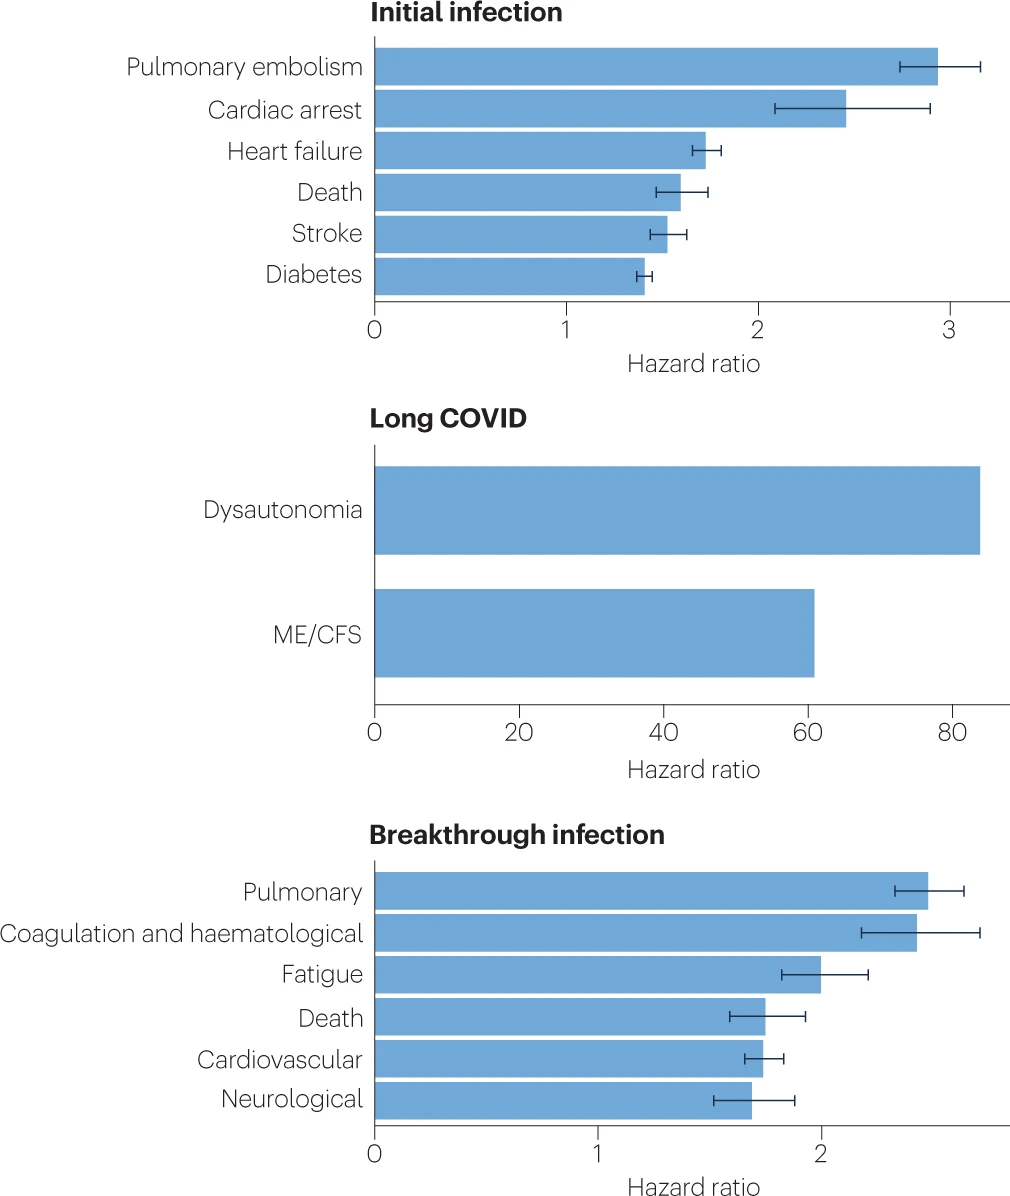
\includegraphics[width=0.75\linewidth]{img/long_COVID.png}
    \caption{The previous study revealed that COVID-19 and long COVID increases the risk of several medical conditions.\cite{b2}}
    \label{fig:long_COVID}
\end{figure}

Additionally, instances of reinfection after initial recovery were observed, with research from the US Department of Veterans Affairs indicating an increased risk of mortality, hospitalization, and postsymptomatic conditions in reinfected patients\cite{b3}.\\

Despite the diminishing immediate threat of COVID-19, the ongoing risks associated with long COVID and reinfection require public attention to COVID-19-related policies and information. The challenges of fake news and misinformation persist as the world transitions into a post-pandemic era coexisting with the virus. Specifically, issues related to long COVID and reinfection remain crucial to misinformation. Therefore, the timely and accurate identification and classification of such misinformation becomes critical.

\subsection{NLP techniques for fake news detection}
NLP techniques combine computational linguistic features and machine learning models to analyze and interpret human language comprehensively. By processing vast amounts of textual data, these techniques can distinguish linguistic patterns, semantic relationships, and sentiment analysis, promoting the identification of misleading content amidst genuine information.\\

Recent language models such as BERT (Bidirectional Encoder Representations from Transformers) and GPT (Generative Pre-trained Transformer) exhibit remarkable capabilities in understanding complex linguistic nuances and contextual meanings within sentences. These models use deep learning architectures to extract complicated semantic information, enabling them to distinguish between genuine and fake narratives effectively.\\

NLP plays an essential role in constantly fighting against misinformation by developing and adapting to emerging false information and linguistic patterns. These techniques help researchers and social platforms enhance the accuracy and efficiency of identifying the spread of fake news.

\section{Goal of This Study}
This study aims to investigate the performance of different deep learning models in detecting misinformation about long COVID. The objective is to develop a scientific and efficient method for identifying fake information in the context of long COVID in the post-pandemic era. Data related to long COVID misinformation were collected from open-source databases and through web crawling processes. These data then underwent a preprocessing phase to clean and refine the text in the dataset. After this, machine learning and various deep learning models were trained and evaluated based on their performance, following the preprocessing step. Additionally, the fuzzy rank-based ensemble approach was employed to combine the strengths of multiple models. Finally, the performance of this ensemble method was compared with the state-of-the-art large language models (LLMs) methods for detecting long COVID misinformation.

\section{Thesis Structure}
Chapter 2 reviews existing literature and previous studies related to fake news detection. It explores various approaches, methodologies, and techniques employed in NLP.
\\

Chapter 3, the method section, details our data collection, preprocessing, and training process. This includes an explanation of how we sourced data related to long COVID and reinfection misinformation from open-source databases and through web crawling. The chapter also discusses the preprocessing techniques we used to clean and refine the collected data, as well as the process of training various machine learning and deep learning models, and the workflow of the ensemble approach used to combine multiple models.
\\

Chapter 4 focuses on implementing the experiment based on the abstracted processes in Chapter 3. It provides insights into the tools, platforms, and technologies used to execute the research experiment effectively. Moreover, Chapter 4 also presents the experiment’s results, evaluating the proposed method’s performance in detecting long COVID misinformation and comparing it with state-of-the-art large language models (LLMs) methods.
\\

Finally, Chapter 5 discusses the principal findings, the implications of the results, and the limitations of the study.

 \newpage
\chapter{Related Work}
\label{ch:relatedwork}

Throughout the COVID-19 pandemic, several research studies have explored the application of machine learning and deep learning techniques to deal with the challenge of the infodemic.\\

For instance, Patwa et al.\cite{b4} have focused exclusively on textual English content, disregarding texts in other languages. The datasets were sourced from publicly available fact-checking websites and social media platforms, targeting fake news. In contrast, real news was collected from the Twitter accounts of 14 official and verified government or medical institutions through web crawling. Each article underwent a manual review for accuracy and relevance.
In the preprocessing phase, the collected data was cleaned by removing all links, non-alphanumeric characters, and English stop words. The term frequency-inverse document frequency (TF-IDF) method was employed for feature extraction. Various machine learning algorithms, including Logistic Regression (LR), Support Vector Machine (SVM) with a linear kernel, Decision Tree (DT), and Gradient Boosting Decision Tree (GDBT), were experimented with the TF-IDF feature. These algorithms were implemented using the sklearn package. Among them, the SVM algorithm achieved the highest test F1 score of 93.32\%, closely followed by Logistic Regression with a 91.96\% F1 score.
This approach to data collection, preprocessing, and model experimentation provides a robust foundation for our study, allowing for meaningful comparisons. The approach also demonstrated the ability of machine learning techniques to address misinformation.\\

Similarly, utilizing the same dataset, Das et al.\cite{b5} employed pre-trained language models (PLMs) for preprocessing and training tasks. Their approach combined predictions from multiple models through a soft voting mechanism, showing admirable results, as evidenced by their success in the CONSTRAINT2021 COVID-19 Fake News Detection competition.
In text preprocessing for fake news detection, they have leveraged various Python libraries to filter out colloquial language, usernames, URLs, and emojis. These preprocessing steps ensure the textual data is clean and suitable for model training.
Their study employed a variety of pre-trained language models, including XLNet, RoBERTa, XLM-RoBERTa, DeBERTa, ERNIE 2.0, and ELECTRA. These models utilized pre-trained weights as their initial starting points, which were then fine-tuned on the specific datasets for the classification task. All textual data was tokenized using the tokenizers corresponding to each pre-trained model, ensuring consistency with the model architectures.
Each model was appended with an additional fully connected layer at the bottom to generate prediction probabilities. Moreover, ensemble methods such as soft and hard voting were applied to combine the predictions of the well-performing models. These ensemble techniques aim to ease the limitations of individual models by balancing their strengths and weaknesses, thereby improving overall performance in fake news detection tasks. This study also highlights the effectiveness of advanced pre-trained language models in enhancing the accuracy of fake news detection.\\

Paka et al. \cite {b6} proposed that more than relying on textual features may be required for accurate fake news classification. 
First, they gathered COVID-19-related tweets from Twitter via Twitter API for their dataset. They comprehensively analyzed the dataset, examining the occurrences of major keywords and the distribution of sentiment and likes across the tweets. This analysis provided valuable insights into the characteristics of the tweets related to COVID-19. 
In addition to textual data, Paka et al. incorporated supplementary information such as the number of likes a tweet received, the presence of external links, and the follower count of the users who posted the tweets. These additional features, categorized as tweet features and user features, enriched the textual dataset and contributed to more information for classification.  
They presented an innovative classification approach utilizing a cross-stitch unit in combination with a Long Short-Term Memory (LSTM) architecture (Fig. \ref{fig:Cross-SEAN.}). The cross-stitch unit was employed to handle tweet and user features, while the LSTM was used to process the textual data. These sections were then concatenated via a fully connected layer. This hybrid model architecture demonstrated the potential benefits of integrating diverse features from social media for fake news detection.
The method proposed by Paka et al. achieved an impressive F1-score of 95.3\%, highlighting the effectiveness of incorporating both textual and non-textual features in improving the accuracy of fake news detection.\\

\begin{figure}
    \centering
    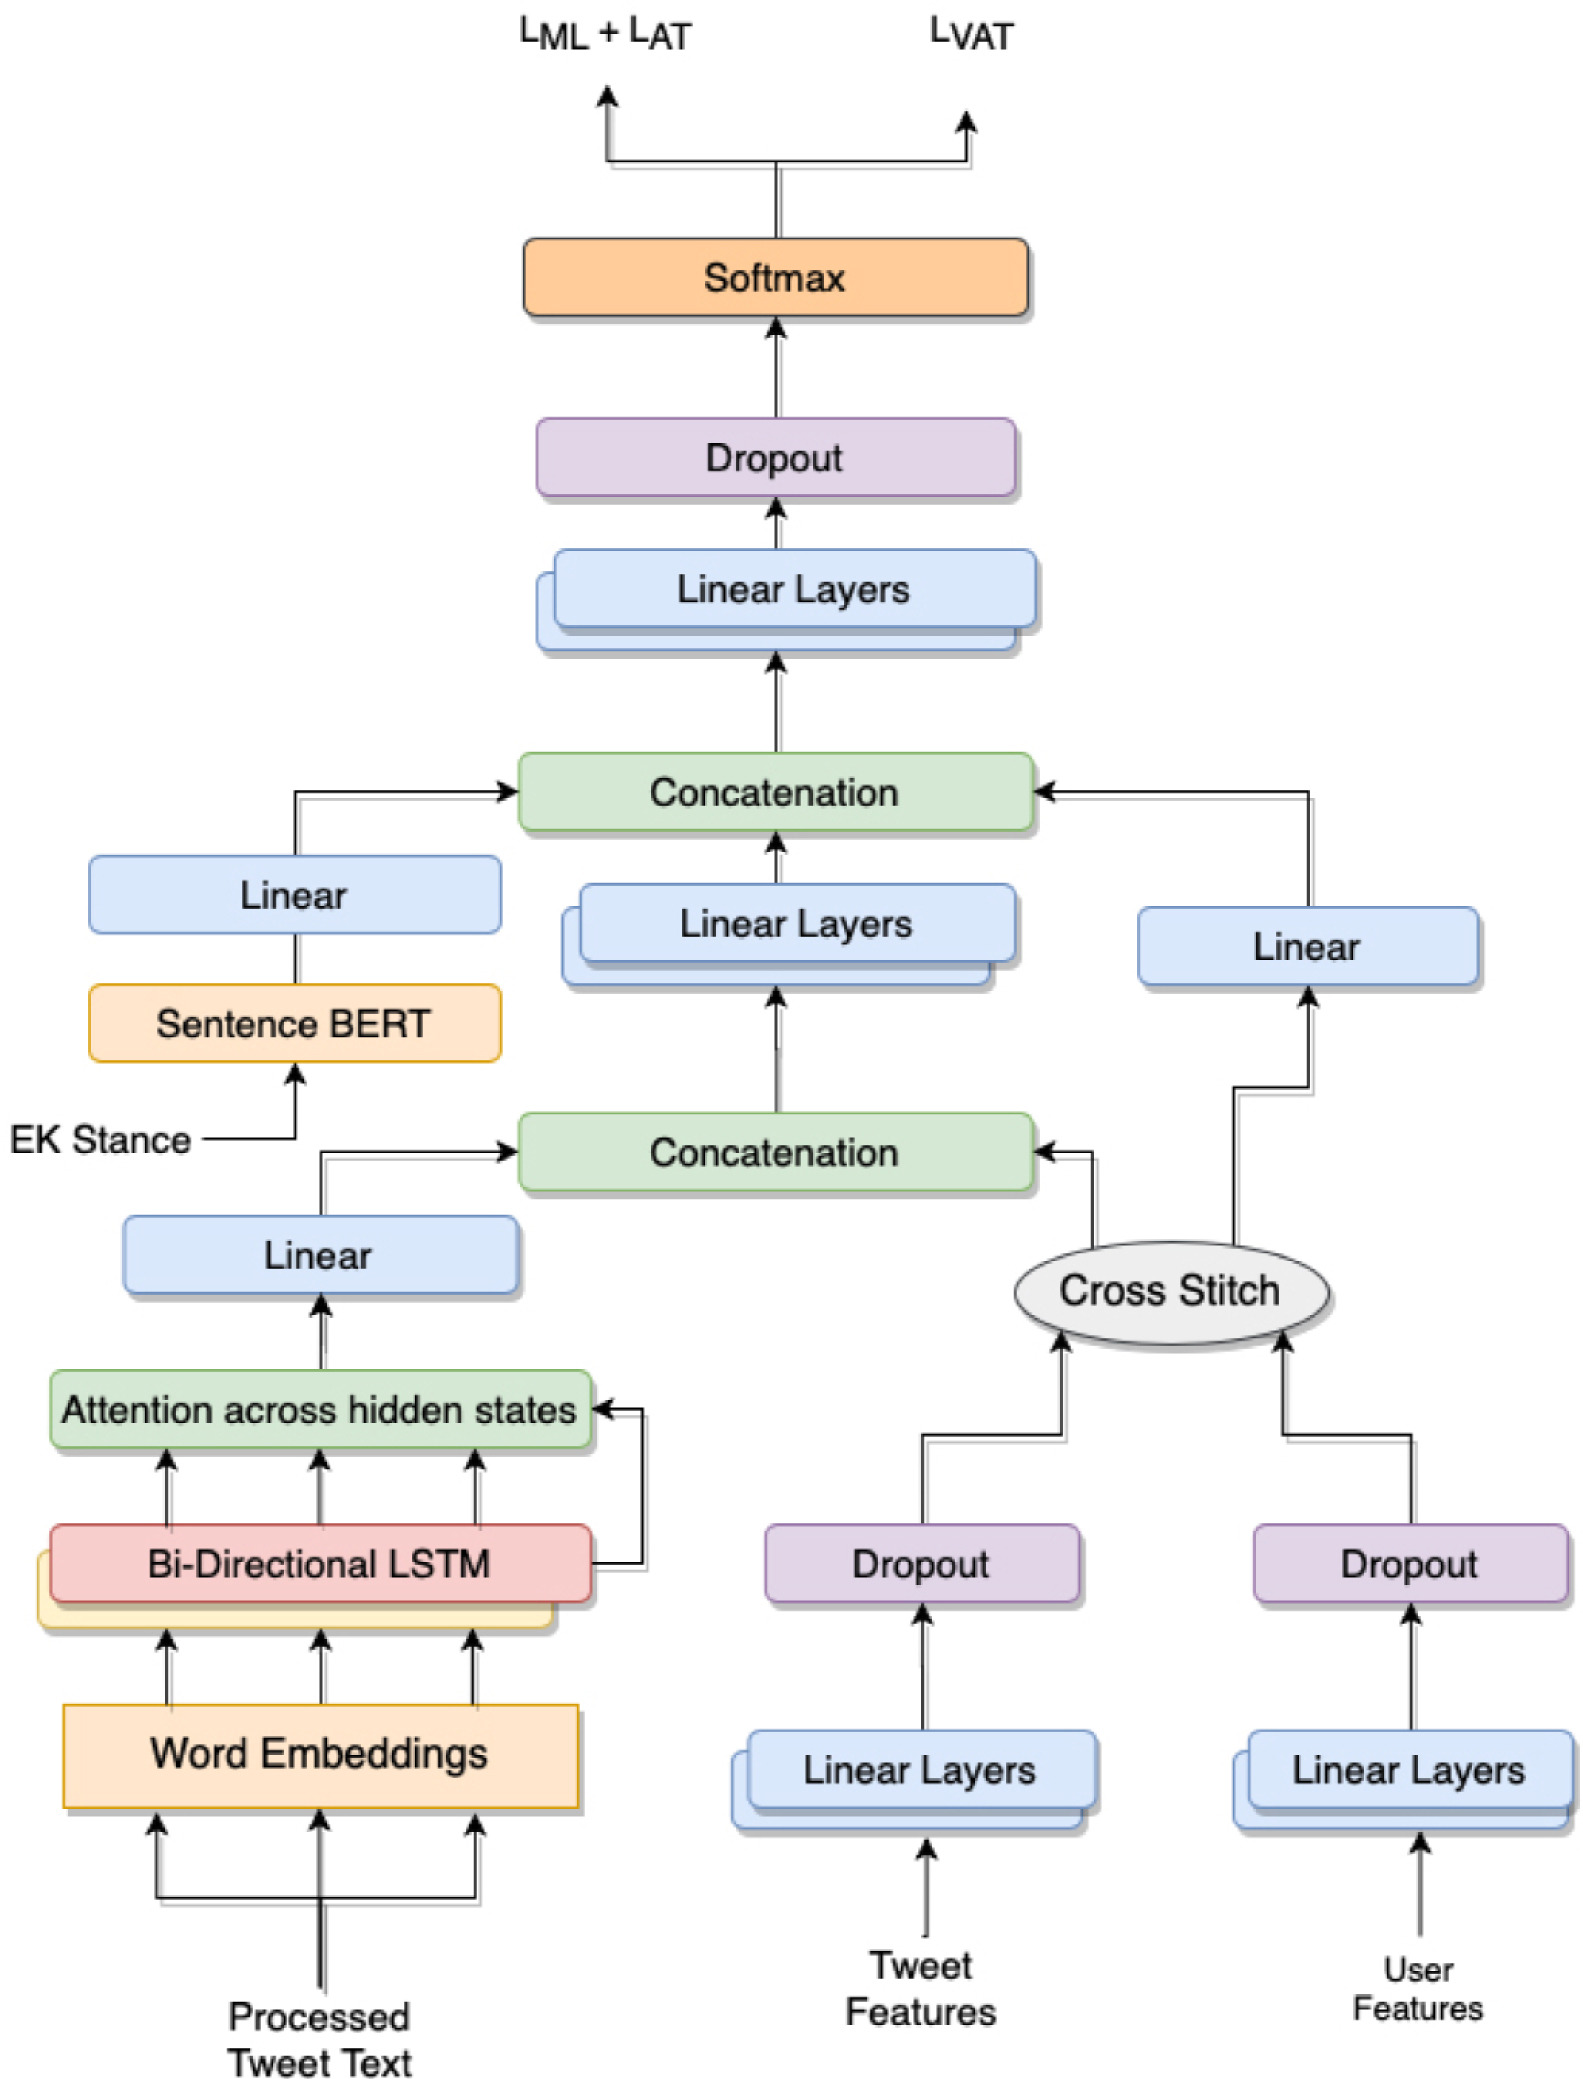
\includegraphics[width=1\linewidth]{img/Cross-SEAN.jpg}
    \caption{The architecture of Cross-SEAN \cite{b6}.}
    \label{fig:Cross-SEAN.}
\end{figure}

Furthermore, research teams focusing on the Chinese language have also made efforts in this domain \cite{b7}. They gathered fact-checked microblogs from Weibo, a popular Chinese social media platform. These microblogs were meticulously labeled and contained various attributes, including blog\_id, date, user\_id, text\_content, number of comments, number of reposts, and number of likes.
Similar to other research, they comprehensively analyzed the collected dataset. The analysis included statistical investigation and the distribution of selected keywords within the dataset (Fig. \ref{fig:CHECKED}). They also presented a visualized word cloud to provide a clearer picture of the prominent terms in the data.
To classify COVID-19 fake news in Chinese text, they utilized advanced deep learning frameworks such as TextCNN and attention-based models like Attention-based TextRNN (Att-TextRNN) and Transformer. These models are well-suited for processing textual data to distinguish between real and fake news.
Their method achieved high performance, with F1-scores reaching 93.8\% with TextCNN and 92.7\% with Transformer. These results underscore the effectiveness of deep learning approaches in handling the intricacies of fake news detection in Chinese text.
These efforts emphasize the global commitment to combating the infodemic.\\
\begin{figure}
    \centering
    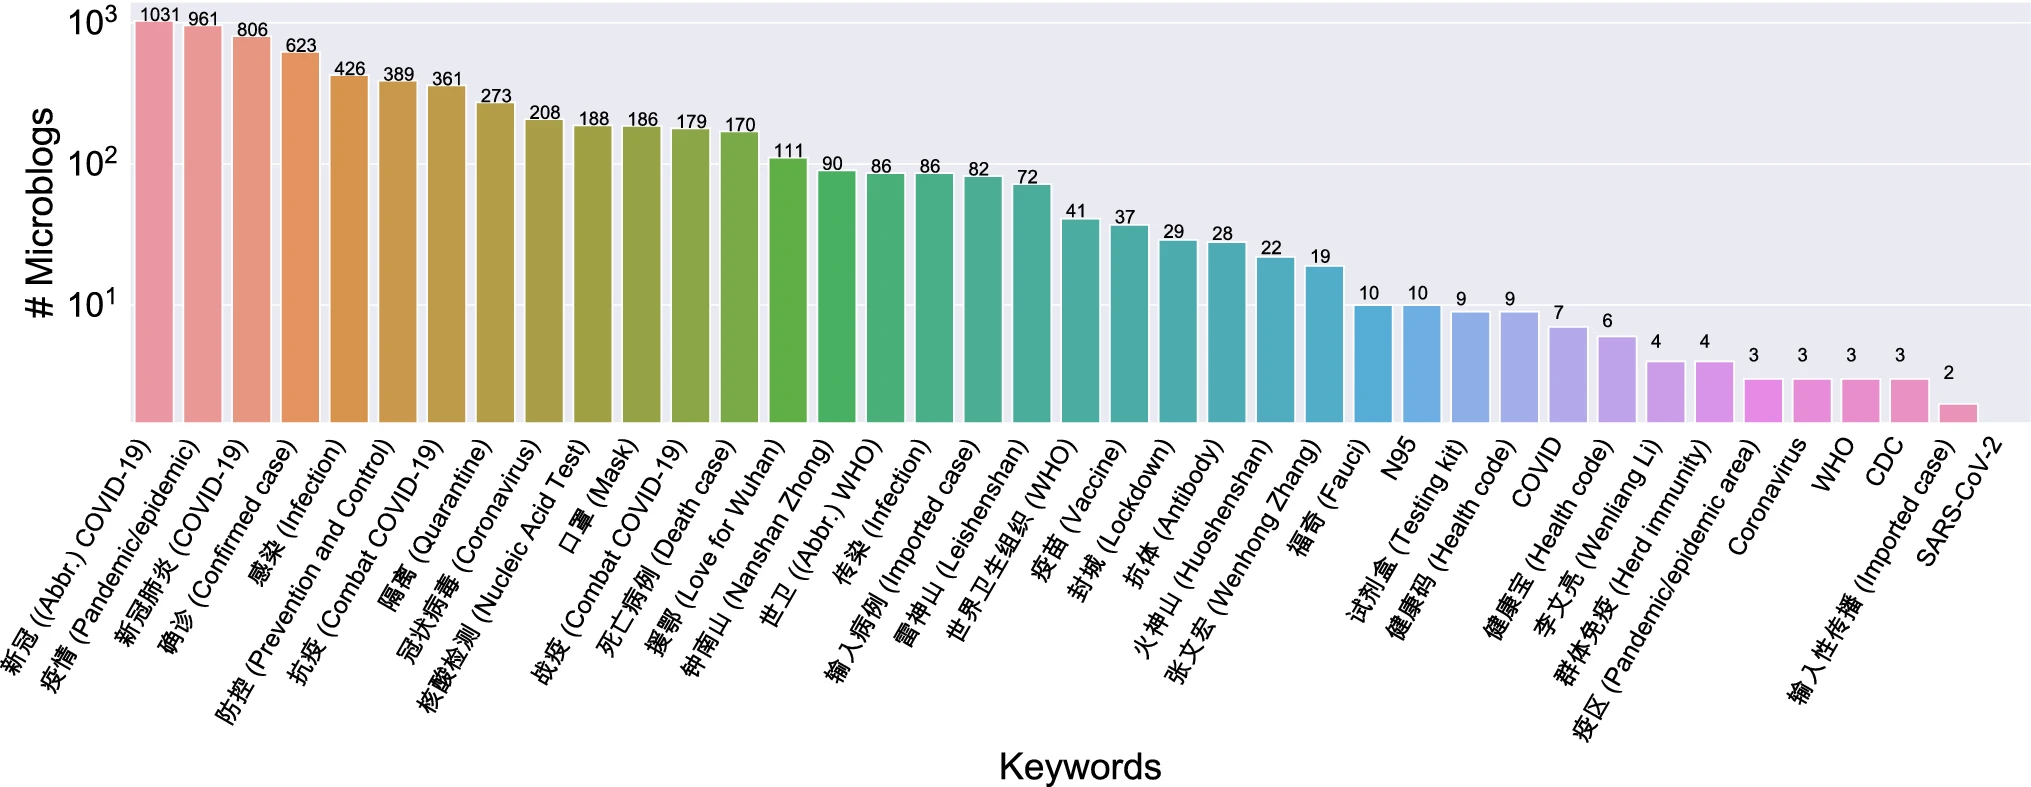
\includegraphics[width=1\linewidth]{img/CHECHED_Keywords.png}
    \caption{Distribution of selected keywords in CHECKED \cite{b7}.}
    \label{fig:CHECKED}
\end{figure}

Additionally, the emergence of large language models (LLMs) based on transformers, such as ChatGPT \cite{b8}, has recently received significant attention. These state-of-the-art models, equipped with advanced natural language understanding capabilities and interactive functionalities, hold enormous potential for developing more powerful tools to combat the spread of misinformation across diverse domains. Their ability to comprehend complex language nuances and engage users in meaningful interactions represents a new stage in advancing fake news detection.
Despite their potential, more studies are needed to explore the capability of LLMs to detect fake news. While LLMs can generate outputs that are coherent and grammatically correct, they may also produce hallucinations (Fig. \ref{fig:Hallucination})—factually incorrect or nonsensical content that appears plausible. This issue raises the importance of evaluating LLMs compared to traditional machine learning algorithms and deep learning models.\\

\begin{figure}
    \centering
    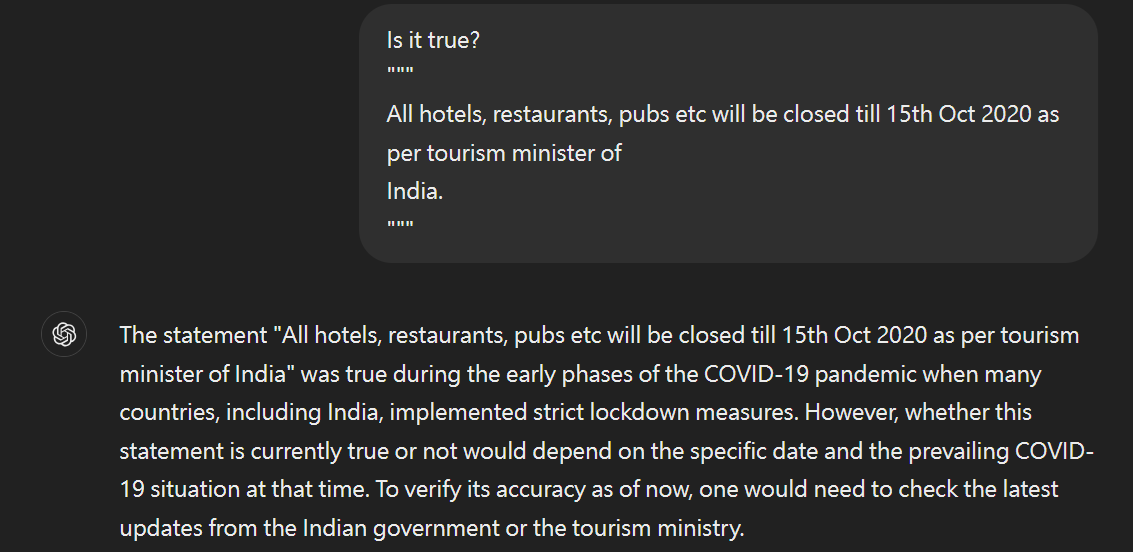
\includegraphics[width=1\linewidth]{img/Hallucination.png}
    \caption{An example of ChatGPT's hallucination, where it incorrectly labels a fake article from a previous study \cite{b4} as true.}
    \label{fig:Hallucination}
\end{figure}
By examining the performance of LLMs against established methods, researchers can better understand the strengths and weaknesses of these models in the context of fake news detection. This comparison is crucial to ensure the reliability and effectiveness of LLMs in real-world applications. \newpage
\chapter{Method}
\label{ch:architecture}
\section{Overview}
The framework of the study consists of four main stages: data collection, data preprocessing, data analysis, and modeling. Each stage is crucial to the analysis and modeling. Initially, data was collected from various open-source datasets. As such sources may contain potential inconsistencies, data preprocessing steps were employed to enhance the cleanliness of the gathered data. After the preprocessing phase, data analysis was conducted to understand the dataset's characteristics better. This includes identifying keyword occurrences and conducting sentiment analysis. Following data analysis, various deep learning models were trained and evaluated. The performance of these models was compared against traditional text classification methods and state-of-the-art LLM models to estimate the effectiveness and performance of different methods within the context. An innovative fusion of ensemble learning techniques was employed to improve detection performance further by using a fuzzy rank-based ensemble approach with the Gompertz function. This approach used a fuzzy rank-based ensemble approach with the Gompertz function. The technique allowed for the adjustment of weights based on the confidence scores of each classifier. The result was more robust and reliable predictions for each sample, which enhanced the overall accuracy of the prediction processes used in the study.

\section{Data Collection}
All text data used in this study were collected from open-source datasets, famous fact-checking websites, and reliable official websites. The gathered data were filtered by using keywords associated with long COVID and reinfection, such as chronic, long-term, persistent, after-effects, sequelae, complications, recovery, post covid, post-covid, omicron, subvariant, reinfection, immune, and variant. The resulting collection formed the dataset for the following experiments. Each sample of data was categorized as either "genuine" or "fake".

\subsection{Open-source datasets}
\textbf{Fighting an Infodemic\cite{b4}:}
An earlier dataset contains topics related to COVID-19 sourced from platforms like Facebook, Twitter,  and websites for fact-checking. This dataset was selected for the \textit{Constraint@AAAI2021 - COVID19 Fake News Detection in English competition}. Only labeled samples from the dataset were used, available on GitHub repository\cite{b9}.\\

\textbf{COVID-19 Twitter Fake News (CTF)\cite{b6}:}
CTF is a dataset focused on tweets from the social media platform Twitter. It includes both labeled and unlabeled data about genuine and fake COVID-19 news. In addition, this dataset contains the tweeters' user-profile features. For this study, only data with label and text content was used.\\

\textbf{Covid-19 heAlthcare mIsinformation Dataset (CoAID)\cite{b10}}:
The CoAID dataset is a collection of COVID-19 fake news sourced from the internet and social media platforms such as Twitter. It includes news articles, user engagements related to fake messages, tweets, and labels.\\


\textbf{Fake news information-broadcasting dataset of COVID-19 (FibVID )\cite{b11}}:
The dataset collects claims from fact-checking websites such as Snopes and Politifact and some related discussions from Twitter. It also assembles user profile data from social media platforms. The FibVID includes COVID and non-COVID topics, separated into four labels. Only samples related to COVID-19 from categories 0 and 1 were used.\\

\textbf{FaCOV\cite{b12}}:
This dataset gathered from 13 English fact-checking websites related to COVID-19, includes article titles, claims made within the articles, external links, and abstracts. The titles and contents from articles were merged, and data with two category labels were used in the experiments.

\subsection{Fact-checking websites}
While open-source databases provide significant help, most contain data only from 2019 to 2021. To conquer this limitation, web scraping and data cleaning techniques were used to gather more recent data. The data collection process comprised the following steps: choosing reliable data sources, extracting text data from websites, and labeling the collected data.\\

\textbf{Source:}
Snopes\cite{b13} and PolitiFact\cite{b14}, both verified by the International Fact-Checking Network (IFCN), were chosen as our primary data sources. This certification assures the audience that the data and labels from these sites have undergone transparent and strict validation processes, enhancing reliability.\\

\textbf{Extraction:}
Given the vast amount of target data, a systematic approach was employed using web scraping to extract articles tagged as  'CORONAVIRUS' and 'COVID-19' from PolitiFact (data up to July 31, 2023) and Snopes (data up to August 31, 2023). The approach was to collect the article contents and the labels for model training. Considering that many articles on fact-checking websites are false news, the clarifications were collected as True samples to balance the ratio if an article was classified as False. From Snopes and PolitiFact, we extracted 1500 and 806 texts, respectively. Later, the collected data were filtered by keywords to align more closely with the research topic. Fig. \ref{fig:fack-checking websites} shows the example of collecting data from PolitiFact.\\

\textbf{Labeling:}
Snopes classifies articles into fourteen labels: lost-legend, labeled-satire, legend, scam, misattributed, correct-attribution, miscaptioned, outdated, unproven, false, mostly false, mixture, mostly-true, and true. On the other hand, PolitiFact categorizes articles into six labels: true, mostly-true, half-true, barely-true, false, and pants-on-fire. According to the study by Khan et al.\cite{b15}, the labels from different databases were reclassified into two categories: genuine and fake. Specifically, the claims labeled as labeled-satire, scam, miscaptioned, misattributed, mostly-false, barely-true, false, and pants-on-fire were categorized as fake. In contrast, those with other labels were categorized as true. Claims with unproven or mixture labels from Snopes were not involved\cite{b11}. 

\begin{figure}
  \centering
  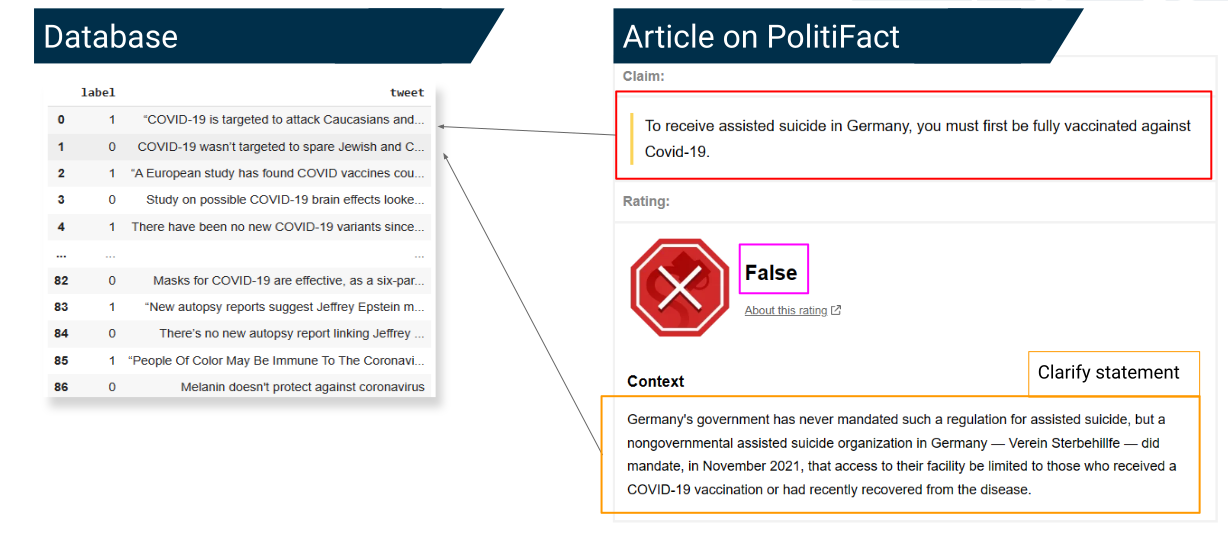
\includegraphics[width=1\columnwidth]{img/fack-checking websites.png}
  \caption{The example of collecting data from fact-checking websites(PolifiFact). } 
  \vspace{-0.4cm}
  \label{fig:fack-checking websites}
\end{figure}

\subsection{Governmental bodies}
Highly reputable government and public organization websites, such as the Centers for Disease Control and Prevention (CDC) and the World Health Organization (WHO), were also considered primary sources. These organizations have consistently supplied up-to-date information and guidelines during the pandemic, so they are widely considered authentic and reliable data sources. 
The articles related to "long COVID" and "Reinfection" were gathered from the COVID-19 sections of these websites. Considering that the original text might have needed longer or included unnecessary details, we utilized ChatGPT \cite{b8} to refine the acquired content. Using ChatGPT, we organized and structured the texts to ensure each claim had an appropriate length and clarity. As a result, each claim was labeled as "genuine" according to its reputable source. After these steps, the dataset used for model training included the latest information.
The table below presents the filtered sample counts from various data sources in Table \ref{tab:data_source}.

\begin{table}[]
    \caption{Sample size from different sources}
    \label{tab:data_source}
    \centering
\begin{tabular}{
>{\columncolor[HTML]{FFFFFF}}c 
>{\columncolor[HTML]{FFFFFF}}c 
>{\columncolor[HTML]{FFFFFF}}c 
>{\columncolor[HTML]{FFFFFF}}c 
>{\columncolor[HTML]{FFFFFF}}c }
\hline
{\color[HTML]{000000} \textbf{Source}} & {\color[HTML]{000000} \textbf{Time until}} & {\color[HTML]{000000} \textbf{Samples}} & {\color[HTML]{000000} \textbf{Fake}} & {\color[HTML]{000000} \textbf{Genuine}} \\ \hline
{\color[HTML]{000000} CTF}             & {\color[HTML]{000000} $\sim$2021}          & {\color[HTML]{000000} 1292}             & {\color[HTML]{000000} 1130}          & {\color[HTML]{000000} 162}              \\
{\color[HTML]{000000} Fighting an Infodemic}            & {\color[HTML]{000000} $\sim$2021}          & {\color[HTML]{000000} 218}              & {\color[HTML]{000000} 62}            & {\color[HTML]{000000} 156}              \\
{\color[HTML]{000000} CoAID}           & {\color[HTML]{000000} $\sim$2020}          & {\color[HTML]{000000} 70}               & {\color[HTML]{000000} 0}             & {\color[HTML]{000000} 70}               \\
{\color[HTML]{000000} FibVID}          & {\color[HTML]{000000} $\sim$2020}          & {\color[HTML]{000000} 615}              & {\color[HTML]{000000} 318}           & {\color[HTML]{000000} 297}              \\
{\color[HTML]{000000} FaCOV}           & {\color[HTML]{000000} $\sim$2021}          & {\color[HTML]{000000} 811}              & {\color[HTML]{000000} 811}           & {\color[HTML]{000000} 0}                \\
{\color[HTML]{000000} PolitiFact}      & {\color[HTML]{000000} $\sim$2023}          & {\color[HTML]{000000} 87}               & {\color[HTML]{000000} 42}            & {\color[HTML]{000000} 45}               \\
{\color[HTML]{000000} Snopes}          & {\color[HTML]{000000} $\sim$2023}          & {\color[HTML]{000000} 15}               & {\color[HTML]{000000} 9}             & {\color[HTML]{000000} 6}                \\
{\color[HTML]{000000} CDC+WHO}         & {\color[HTML]{000000} $\sim$2023}          & {\color[HTML]{000000} 58}               & {\color[HTML]{000000} 0}             & {\color[HTML]{000000} 58}               \\ \hline
{\color[HTML]{000000} Total}           & {\color[HTML]{000000} }                    & {\color[HTML]{000000} 3166}             & {\color[HTML]{000000} 2372}          & {\color[HTML]{000000} 794}              \\ \hline
\end{tabular}
\end{table}

\section{Data Preprocessing}
This study executed three data preprocessing steps to ensure the integrity of the gathered dataset. Firstly, duplicate entries were removed by cross-referencing the merged open-source datasets with existing ones. This step eliminated redundancy, reinforcing confidence in data quality and preventing potential influences on subsequent model training and analysis. Secondly, emojis and external links (URLs), commonly found in social media posts, were cleaned to enhance clarity. Thirdly, label encoding was performed, with '0' representing genuine news and '1' representing fake news. Stratified sampling was employed, assigning 10\% of the data for testing and 90\% for training. This approach ensured consistent label proportions in both sets, reducing the potential shortage of genuine samples that might arise from random sampling.

\subsection{Remove duplicate entries}
To ensure the absence of duplicate entries in the merged open-source datasets, we cross-referenced the data with existing open-source datasets. Any identified duplicate samples were eliminated to reduce redundancy, reinforcing confidence in the data quality and preventing potential influences on the following model training and analysis performance.
\subsection{Remove emojis and URLs}
During the preprocessing phase, social media posts and articles, which frequently include emojis and external links (URLs), were processed to enhance the clarity of the dataset in distinguishing between genuine and fake news. The Tweet-preprocessor package\cite{b5} was employed to remove emojis and URLs from the texts (Fig. \ref{fig:preprocessing}).

\begin{figure}
  \centering
  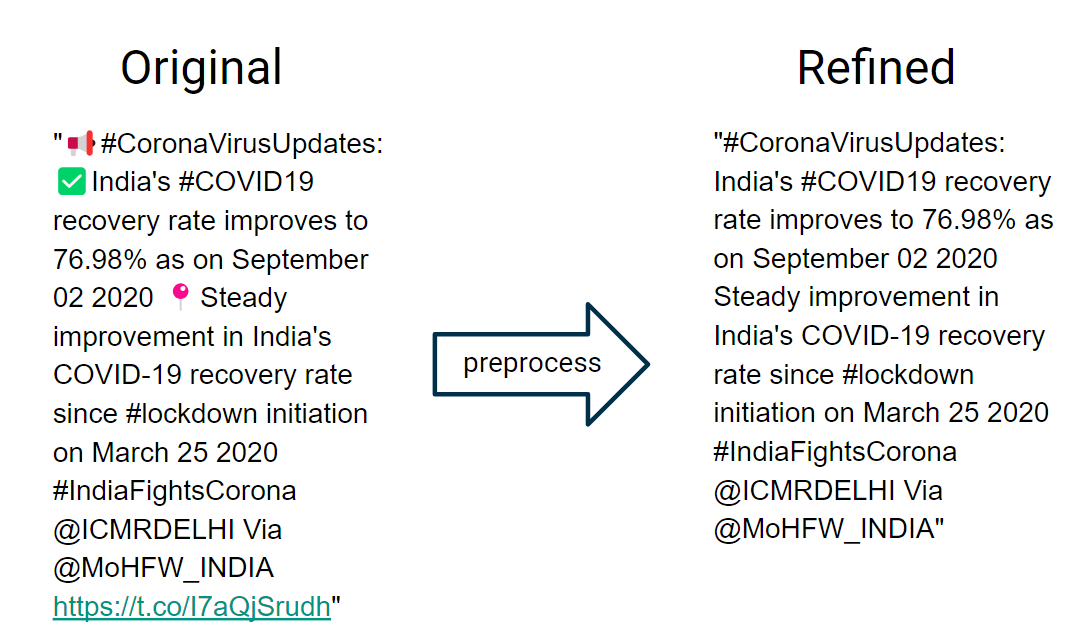
\includegraphics[width=1\columnwidth]{img/preprocessing.png}
  \caption{The example for removing emojis and URLs.} 
  \vspace{-0.4cm}
  \label{fig:preprocessing}
\end{figure}

\subsection{Label encoding}
All the labels were encoded as '0' (stands for genuine) and '1' (stands for fake), respectively. The distribution of our dataset is illustrated in Fig. \ref{fig:data distribution}. As the public data sources exhibited a bias towards the 'fake' category, an imbalanced label distribution was observed in the dataset. To ensure fairness, we employed stratified sampling, allocating 10\% of the data for testing and 90\% for training. This sampling approach ensures consistent label proportions in both the test and training sets, preventing the potential insufficient of genuine samples that may arise from random sampling.



\begin{figure}
  \centering
  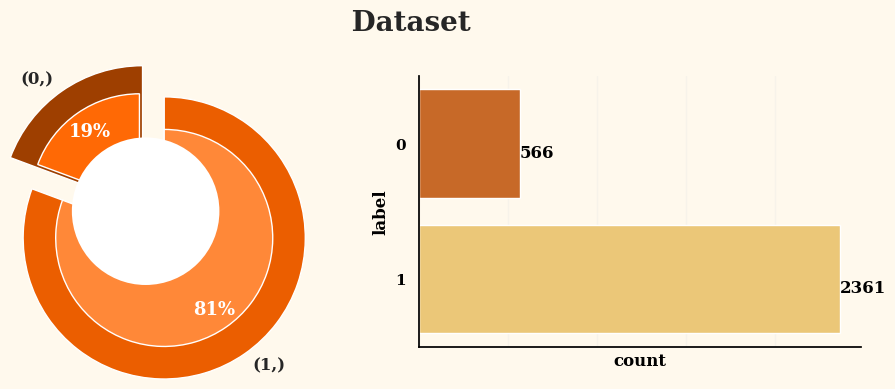
\includegraphics[width=1\columnwidth]{img/data distribution.png}
  \caption{Label distribution after preprocessing.} 
  \vspace{-0.4cm}
  \label{fig:data distribution}
\end{figure}

\section{Data Analysis}
The data analysis uncovered notable keyword occurrences, sentiment, and subjectivity patterns. This examination aimed to gain deeper insights into the experiment dataset and identify differences between genuine and fake articles. By analyzing these patterns, we sought to understand how specific keywords, emotional tones, and levels of subjectivity could differentiate between real and false information in the context of long COVID and reinfections.
\subsection{Keywords occurrences}
Analysis of the frequency of specific keywords in the data reveals interesting patterns. In Fig. \ref {fig:keywords_by_label}, more than half of the fake samples contain the term 'immune', a term rarely found in the genuine category. On the other hand, the term 'recovery' is primarily seen in genuine samples, but a similar proportion of fake samples also use it. Further, keywords such as 'variant', 'complication', and 'chronic' also occur at higher frequencies in fake samples, arousing people's curiosity. This suggests that such words are often used to propagate fake news.

\begin{figure}
    \centering
    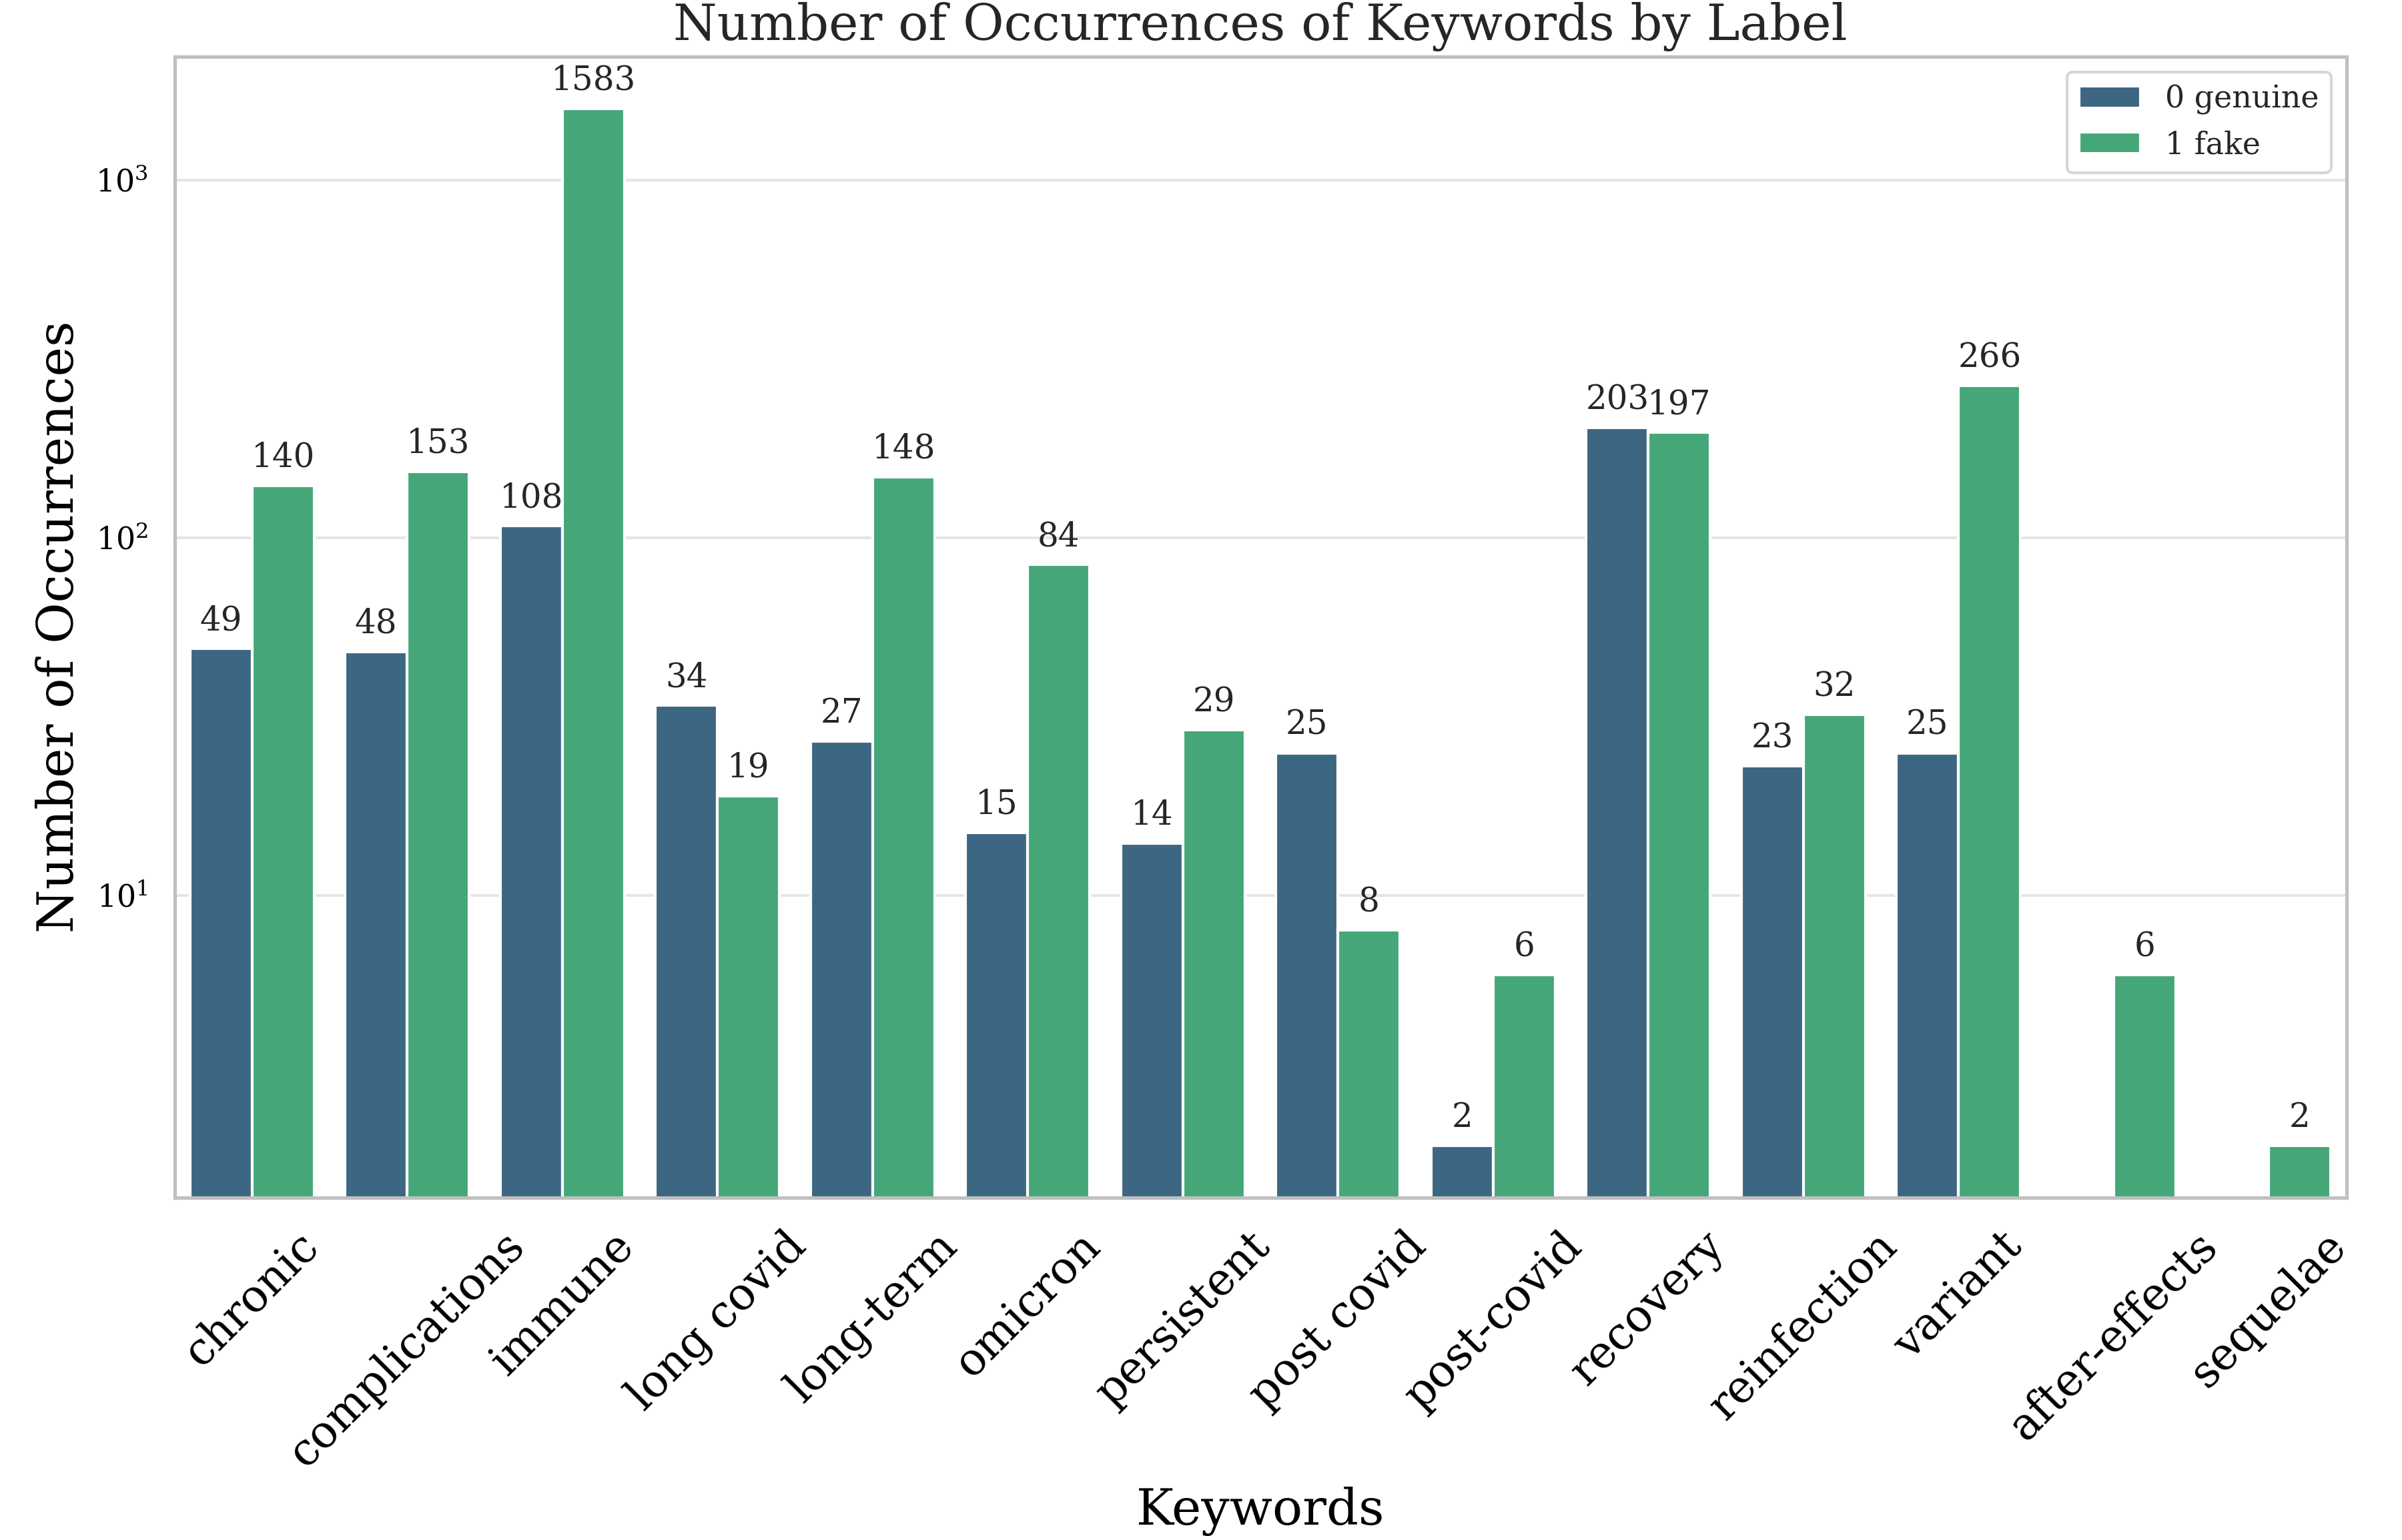
\includegraphics[width=1\linewidth]{img/keywords_by_label.png}
    \caption{Number of keywords occurrences by label}
    \label{fig:keywords_by_label}
\end{figure}

\subsection{Sentiment analysis}
To get a deeper insight into the textual data gathered from fact-checking websites and open-source databases, we utilized the package called TextBlob \cite{b16} for sentiment analysis. Sentiment analysis can reveal whether the textual content of an article is negative, positive, or neutral. Moreover, it can estimate the subjectivity of the text, indicating whether the claim is based on facts or the writer's opinions. \\

\textbf{Polarity:}
Using the TextBlob package, we obtained polarity values ranging from -1 to 1, representing the sentiment from entirely negative to totally positive.To differentiate various sentiment degrees, we categorized sentiments based on polarity into five groups as follows:
\begin{itemize}
\item Strongly Negative: -1 $\leq$ Polarity $<$ -0.5
\item Slightly Negative: -0.5 $\leq$ Polarity $<$ -0.1
\item Neutral: -0.1 $\leq$ Polarity $<$ 0.1
\item Slightly Positive: 0.1 $\leq$ Polarity $<$ 0.5
\item Strongly Positive: 0.5 $\leq$ Polarity $\leq$ 1
\end{itemize}

As Fig. \ref {fig:sentiment} shows, most content is primarily categorized as 'neutral' no matter whether the text is fake or genuine. 65\% of the content in fake texts falls into this category, while 53\% of the content in genuine texts does so. Besides, genuine texts show a higher proportion (36\%) in the "slightly positive" category compared to fake texts (24\%), suggesting that genuine content frequently uses more positive language and favorable terms. The distribution between the two labels is similar in terms of the other sentiment categories ('strongly negative,' 'slightly negative,' and 'strongly positive').\\

\begin{figure}
    \centering
    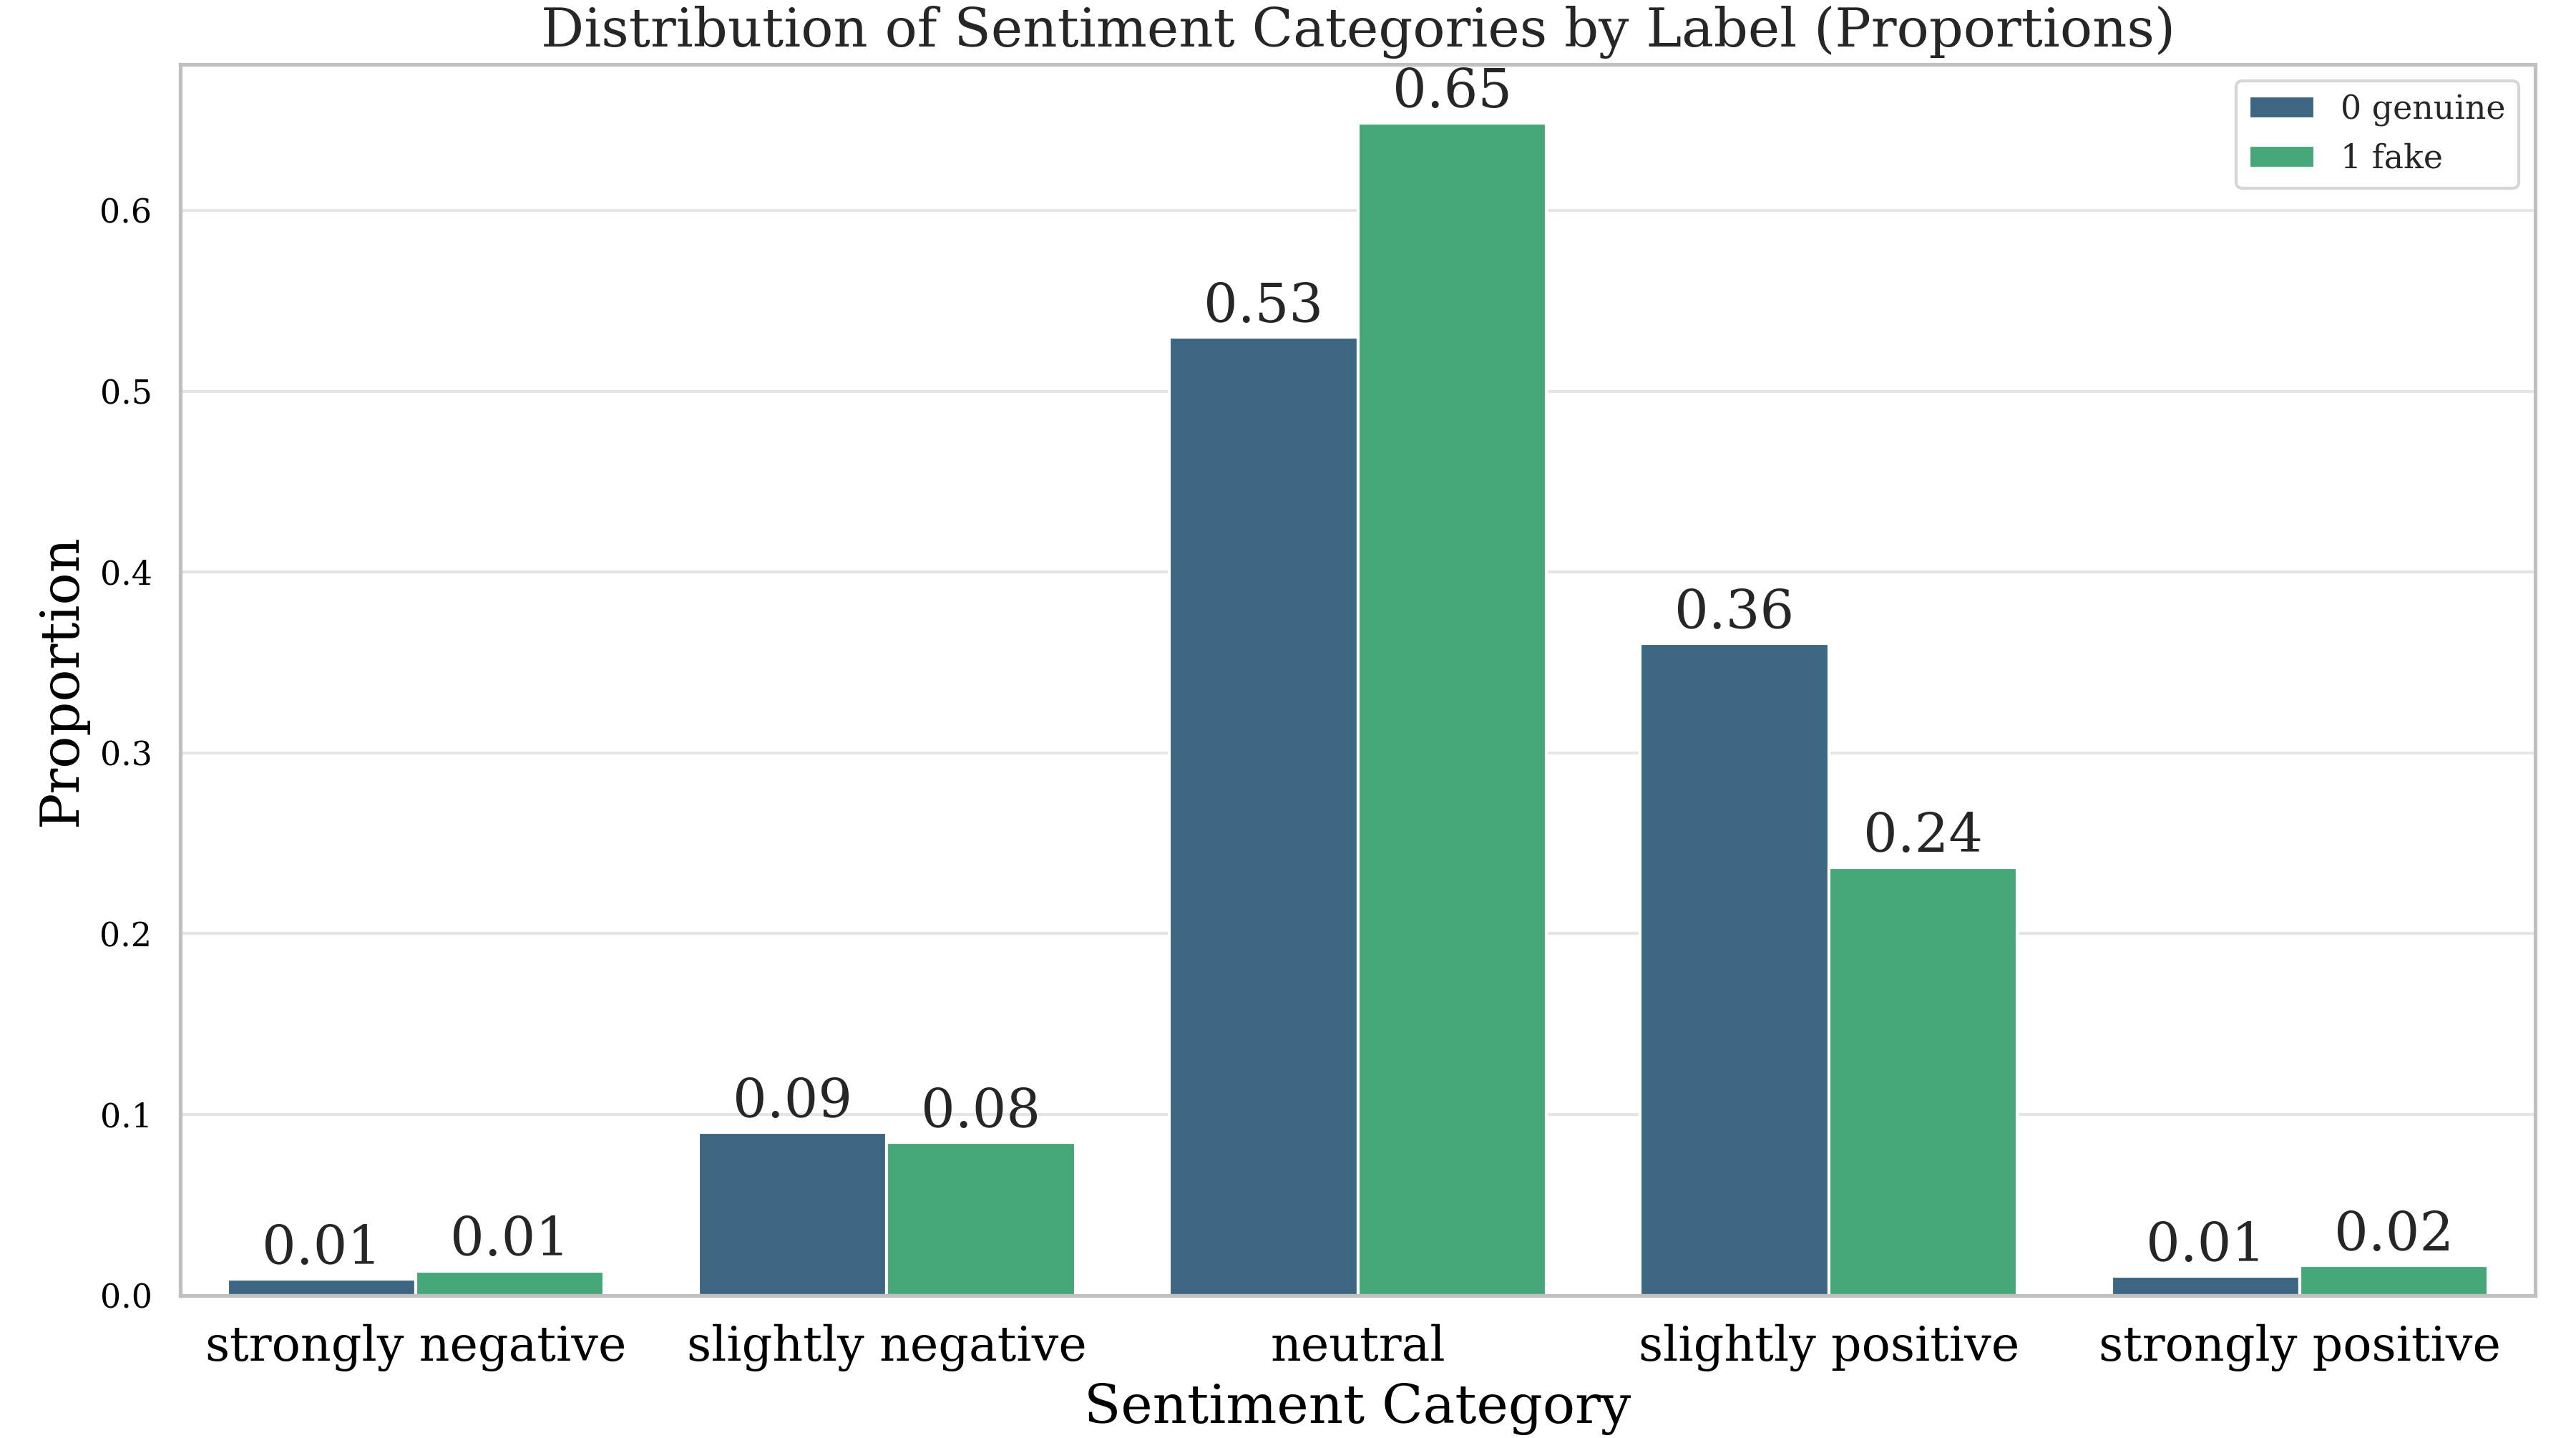
\includegraphics[width=1\linewidth]{img/Sentiment.png}
    \caption{Data distribution (percentage) of different sentiment polarity groups}
    \label{fig:sentiment}
\end{figure}

\textbf{Subjectivity:}
In addition to sentiment analysis, TextBlob provides a subjectivity score ranging from 0 to 1, indicating the degree of subjectivity within the text, ranging from entirely objective to entirely subjective. We categorized the degree of subjectivity into the following five groups:

\begin{itemize}
\item Low Subjectivity: 0 $\leq$ Subjectivity $<$ 0.2
\item Medium-Low Subjectivity: 0.2 $\leq$ Subjectivity $<$ 0.4
\item Medium Subjectivity: 0.4 $\leq$ Subjectivity $<$ 0.6
\item Medium-High Subjectivity: 0.6 $\leq$ Subjectivity $<$ 0.8
\item High Subjectivity: 0.8 $\leq$ Subjectivity $\leq$ 1
\end{itemize}

As illustrated in Fig. \ref {fig:subjectivity}, there is a similarity in the distribution of subjectivity between genuine and fake texts, both primarily falling under the 'medium subjectivity' category. Genuine texts account for 38\% of their content in this category, while fake texts account for 37\%. In the "low subjectivity" category, there is a 5\% higher of fake texts than genuine texts. In the 'medium-high subjectivity' category, genuine texts exceed fake texts by 3\%. \\

These findings emphasize the need for more precise methods to distinguish between genuine and fake news texts because even though some minor differences are observed in the distribution of sentiment polarity and subjectivity between genuine and fake texts, these differences may not serve as definitive classification criteria. Moreover, sentiment analysis faces challenges in natural language understanding, such as accurately identifying sarcasm. Therefore, more precise approaches, such as machine learning algorithms and deep learning models, are required to distinguish genuine from fake news concerning long COVID and reinfections.

\begin{figure}
    \centering
    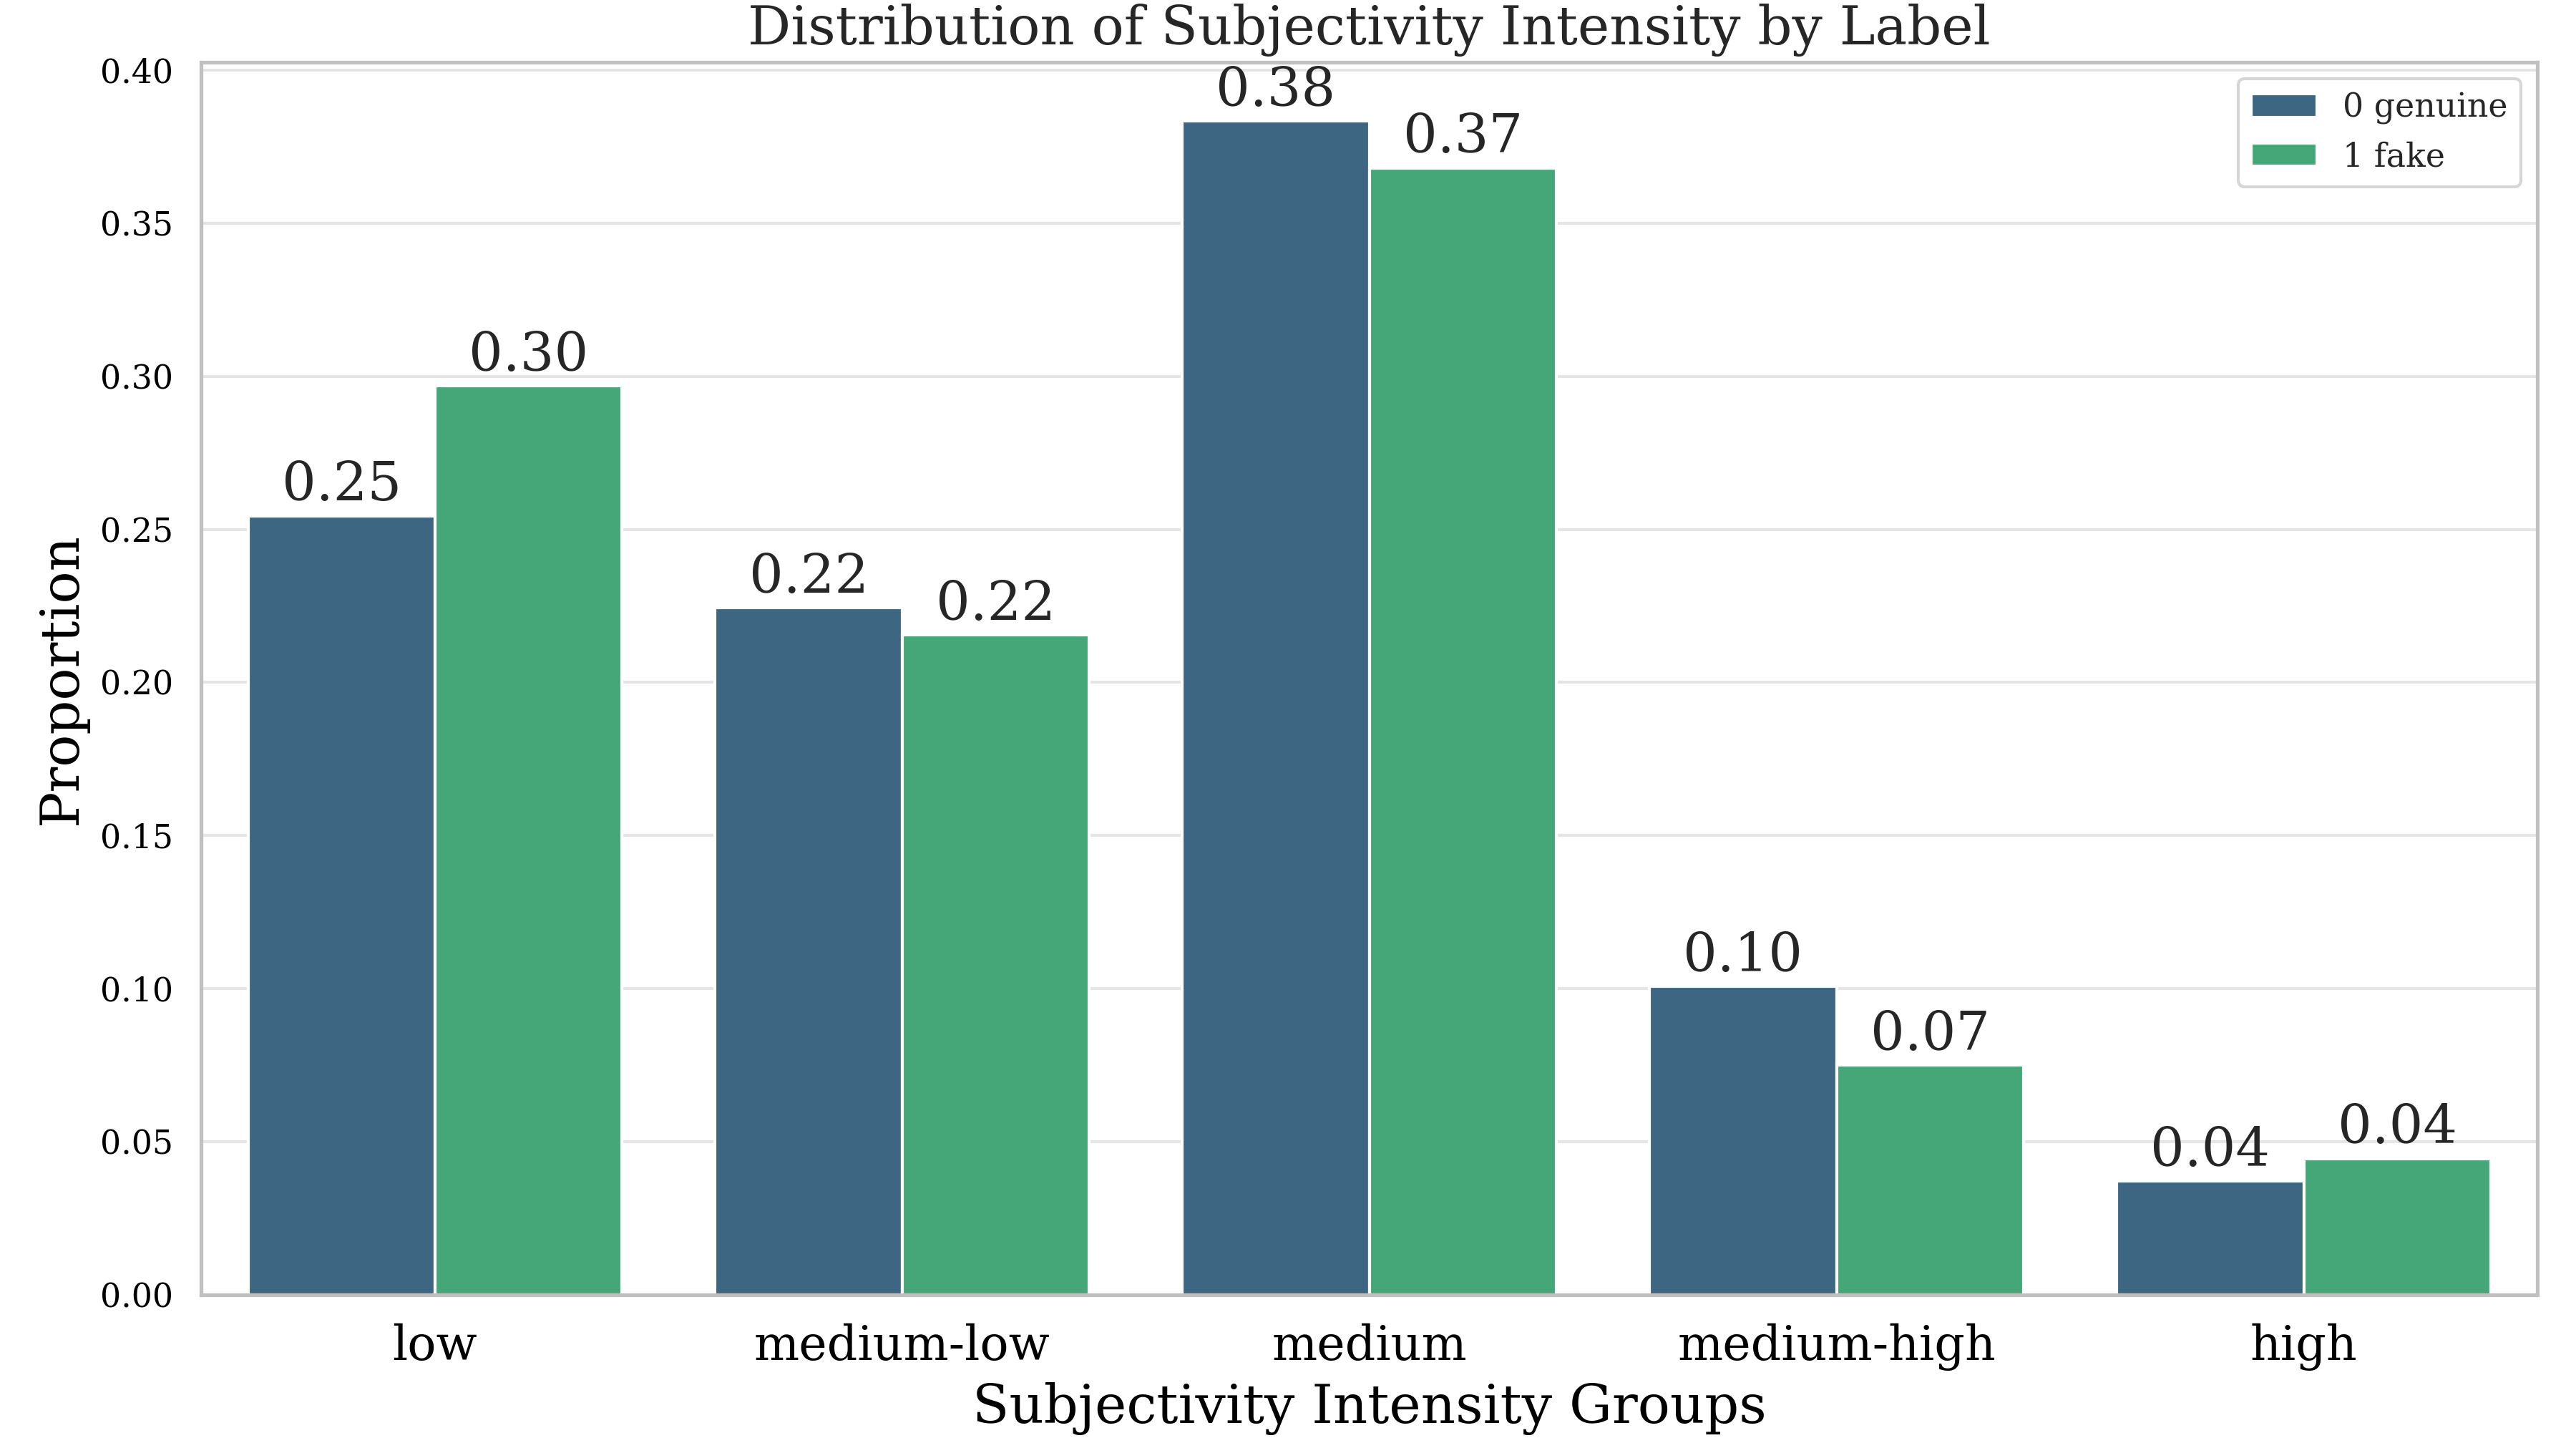
\includegraphics[width=1\linewidth]{img/Subjectivity.png}
    \caption{Data distribution (percentage) of different subjectivity groups}
    \label{fig:subjectivity}
\end{figure}

\section{Models}
In this study, a comprehensive comparison was conducted using various models. Conventional machine learning algorithms that utilized text content or content-based features were employed to establish a baseline. Additionally, attention-based models, from hierarchical neural networks to pre-trained language models, were also explored to take advantage of their advanced capabilities in handling complex textual data. Furthermore, embedding models based on large language models (LLMs) were used to compare the performance between open-source deep models and fee-required models. This approach allowed us to evaluate the effectiveness of different methodologies in distinguishing between genuine and fake news articles, particularly in the context of long COVID and reinfections.

\subsection{TF-IDF with SVM}
To establish a baseline model for text classification, this study initially chose the Support Vector Machine (SVM)\cite{b17}, commonly recognized as a robust baseline model in the field. 
Linear classifiers, such as SVM, provide a straightforward strategy for binary classification tasks by finding the optimal hyperplane that separates two classes in the feature space. 
This study applied the SVM model using uni-gram TF-IDF features generated from the training set data. These features were derived from a bag-of-words approach where each word or token in the text was treated as a separate feature. The TF-IDF (Term Frequency-Inverse Document Frequency) technique was employed to weigh the importance of each word in the document against its frequency in the entire corpus. The TF-IDF score can be represented as the following equation:
\begin{equation}
    TF\text{-}IDF(t,d)=TF(t,d)×IDF(t)
\end{equation}
which consists of two following components:
\begin{equation}
    TF(t,d) = \frac{\text{frequency of the term }\displaystyle t \text{ in the document } \displaystyle d }{\text{number of terms in } \displaystyle d} 
\end{equation}

\begin{equation}
    IDF(t) = log_{e}\left(  \frac{\text{numbers of documents}}{\text{numbers of documents with }t}\right)
\end{equation}
The performance of the SVM classifier was evaluated by comparing its accuracy, precision, recall, and F1-score with those of deep learning models. This comparison helps validate whether deep models are correctly fine-tuned and employed for text classification tasks\cite{b18}.
%https://arxiv.org/pdf/1806.06407
\subsection{Content-based features with XGBoost}
The method combined XGBoost with content-based features, such as frequency of sectarian words, the strength of quoted sources/attribution, and linguistic features, was included in this study\cite{b19}. Generally, articles exhibiting excessively sectarian discourse are deemed less credible. The frequency of sectarian words was calculated by dividing the number of sectarian words by the total number of words in each article.
The strength of source attribution is crucial for determining the trustworthiness of information. This feature measures how well sources are quoted or attributed in the news. Strong and clear source attributions in news articles might enhance credibility.
Additionally, the frequency of assertive verbs, which indicate the degree of certainty in a statement, and factive verbs, which presuppose the truth of a proposition, were measured. High frequencies of these verbs can provide insights into the tone and reliability.
However, due to the limitations of our collected data, the inconsistency score, which measures the consistency of information within and across articles, could not be computed. Therefore, our comparison focused solely on content-based features. These extracted features were then used to train an XGBoost model.

\subsection{HAN}
Hierarchical Attention Networks (HAN)\cite{b20} incorporate attention mechanisms at multiple levels, specifically at the word and sentence levels, to capture diverse hierarchical structures of documents. The authors employed Recurrent Neural Networks (RNNs) combined with word-attention and sentence-attention layers for text classification. This architecture shown in Fig. \ref{fig:HAN} yielded state-of-the-art results across six datasets.

\begin{figure}
    \centering
    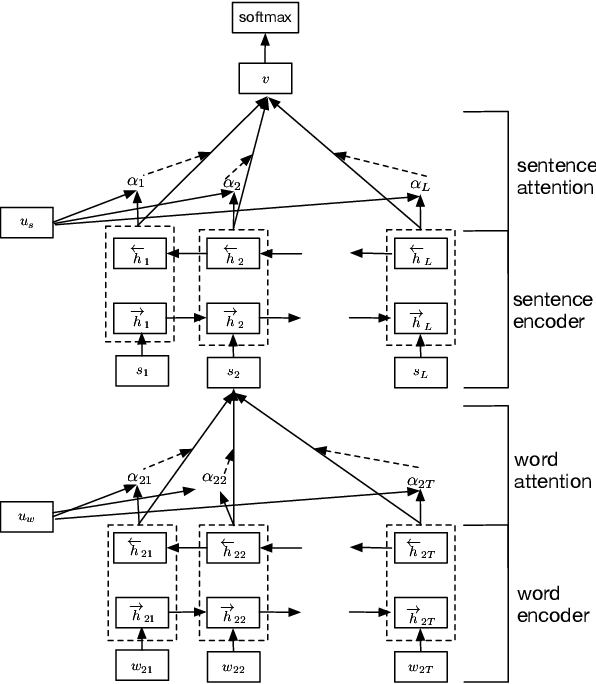
\includegraphics[width=1\linewidth]{img/HAN.png}
    \caption{The architecture of Hierarchical Attention Networks (HAN)\cite{b20}}
    \label{fig:HAN}
\end{figure}

\subsection{BERT}
Bidirectional Encoder Representations from Transformers (BERT)\cite{b21} was a state-of-the-art pre-trained language model based on the Transformer\cite{b22} architecture developed by Google in 2018. It has been trained on massive volumes of text data using masked language modeling and next-sentence prediction techniques. Through self-attention mechanisms, BERT can generate contextualized word representations by considering each word's surrounding context. This contextual information helps BERT to understand the meaning of words in a given sentence more accurately. Due to its robustness and effectiveness, BERT has become one of the most popular and widely used language models in NLP fields. It finds applications across various NLP tasks such as classification, named entity recognition, and question answering.

\subsection{RoBERTa}
In 2019, Facebook introduced the Robustly Optimized BERT Pretraining Approach (RoBERTa)\cite{b23} as an enhancement to the BERT model. RoBERTa was trained on a significantly larger dataset than BERT, allowing it to capture a more comprehensive understanding of language. Unlike BERT, RoBERTa eliminated the next sentence prediction task during pretraining, focusing solely on masked language modeling. Additionally, RoBERTa implemented optimization techniques such as dynamic masking and training with larger batch sizes to improve its performance further. In comparative studies by Facebook, RoBERTa outperformed BERT across various NLP tasks.

\subsection{DeBERTa}
Decoding-enhanced BERT with Disentangled Attention (DeBERTa)\cite{b24}  introduced a novel attention mechanism known as "disentangled attention" to improve upon the original self-attention mechanism. Additionally, it employs the mask decoder and incorporates token absolute positioning to enhance sequence information capturing and pre-training. These enhancements strengthen the model's understanding of text structure and context. In evaluations across various NLP tasks, DeBERTa has demonstrated superior performance to other pre-trained models like BERT and RoBERTa, demonstrating its effectiveness and advancements in NLP research.

\subsection{XLNet}
Introduced by Google in 2019, XLNet\cite{b25} is a pre-trained language model that introduced the concept of "permutation language modeling." This approach aimed to enhance bidirectional contextual understanding within language models. With the Transformer-XL architecture trained on extensive text data, XLNet conquered challenges related to understanding long texts. Furthermore, XLNet overcame certain limitations observed during pre-training from BERT, exhibiting its superior performance compared to other pre-trained language models like RoBERTa and BERT across multiple NLP benchmark tasks.

\subsection{LLMs}
The recent success of large language models (LLMs) has significantly impacted applications within the field of NLP. This study used OpenAI's "text-embedding-ada-002"\cite{b26} and Google's Gemini embedding models\cite{b27} to transform the training set data into embedding. Embedding captures various attributes of a word through vectors, which are lists of floating-point numbers. The relationship between two vectors is measured by their distance, where small distances indicate high relevance and large distances indicate low relevance. Words with similar meanings are typically close to each other in the embedding space. Additionally, arithmetic operations can be performed on word embeddings to yield meaningful results. For instance, the embedding of 'king' - the embedding of 'man' + the embedding of 'woman' is approximately equal to the embedding of 'queen'. Fig. \ref{fig:ada_embedding} shows the visualized embedding of text-embedding-ada-002 using t-SNE\cite{b28}\\

\begin{figure}
    \centering
    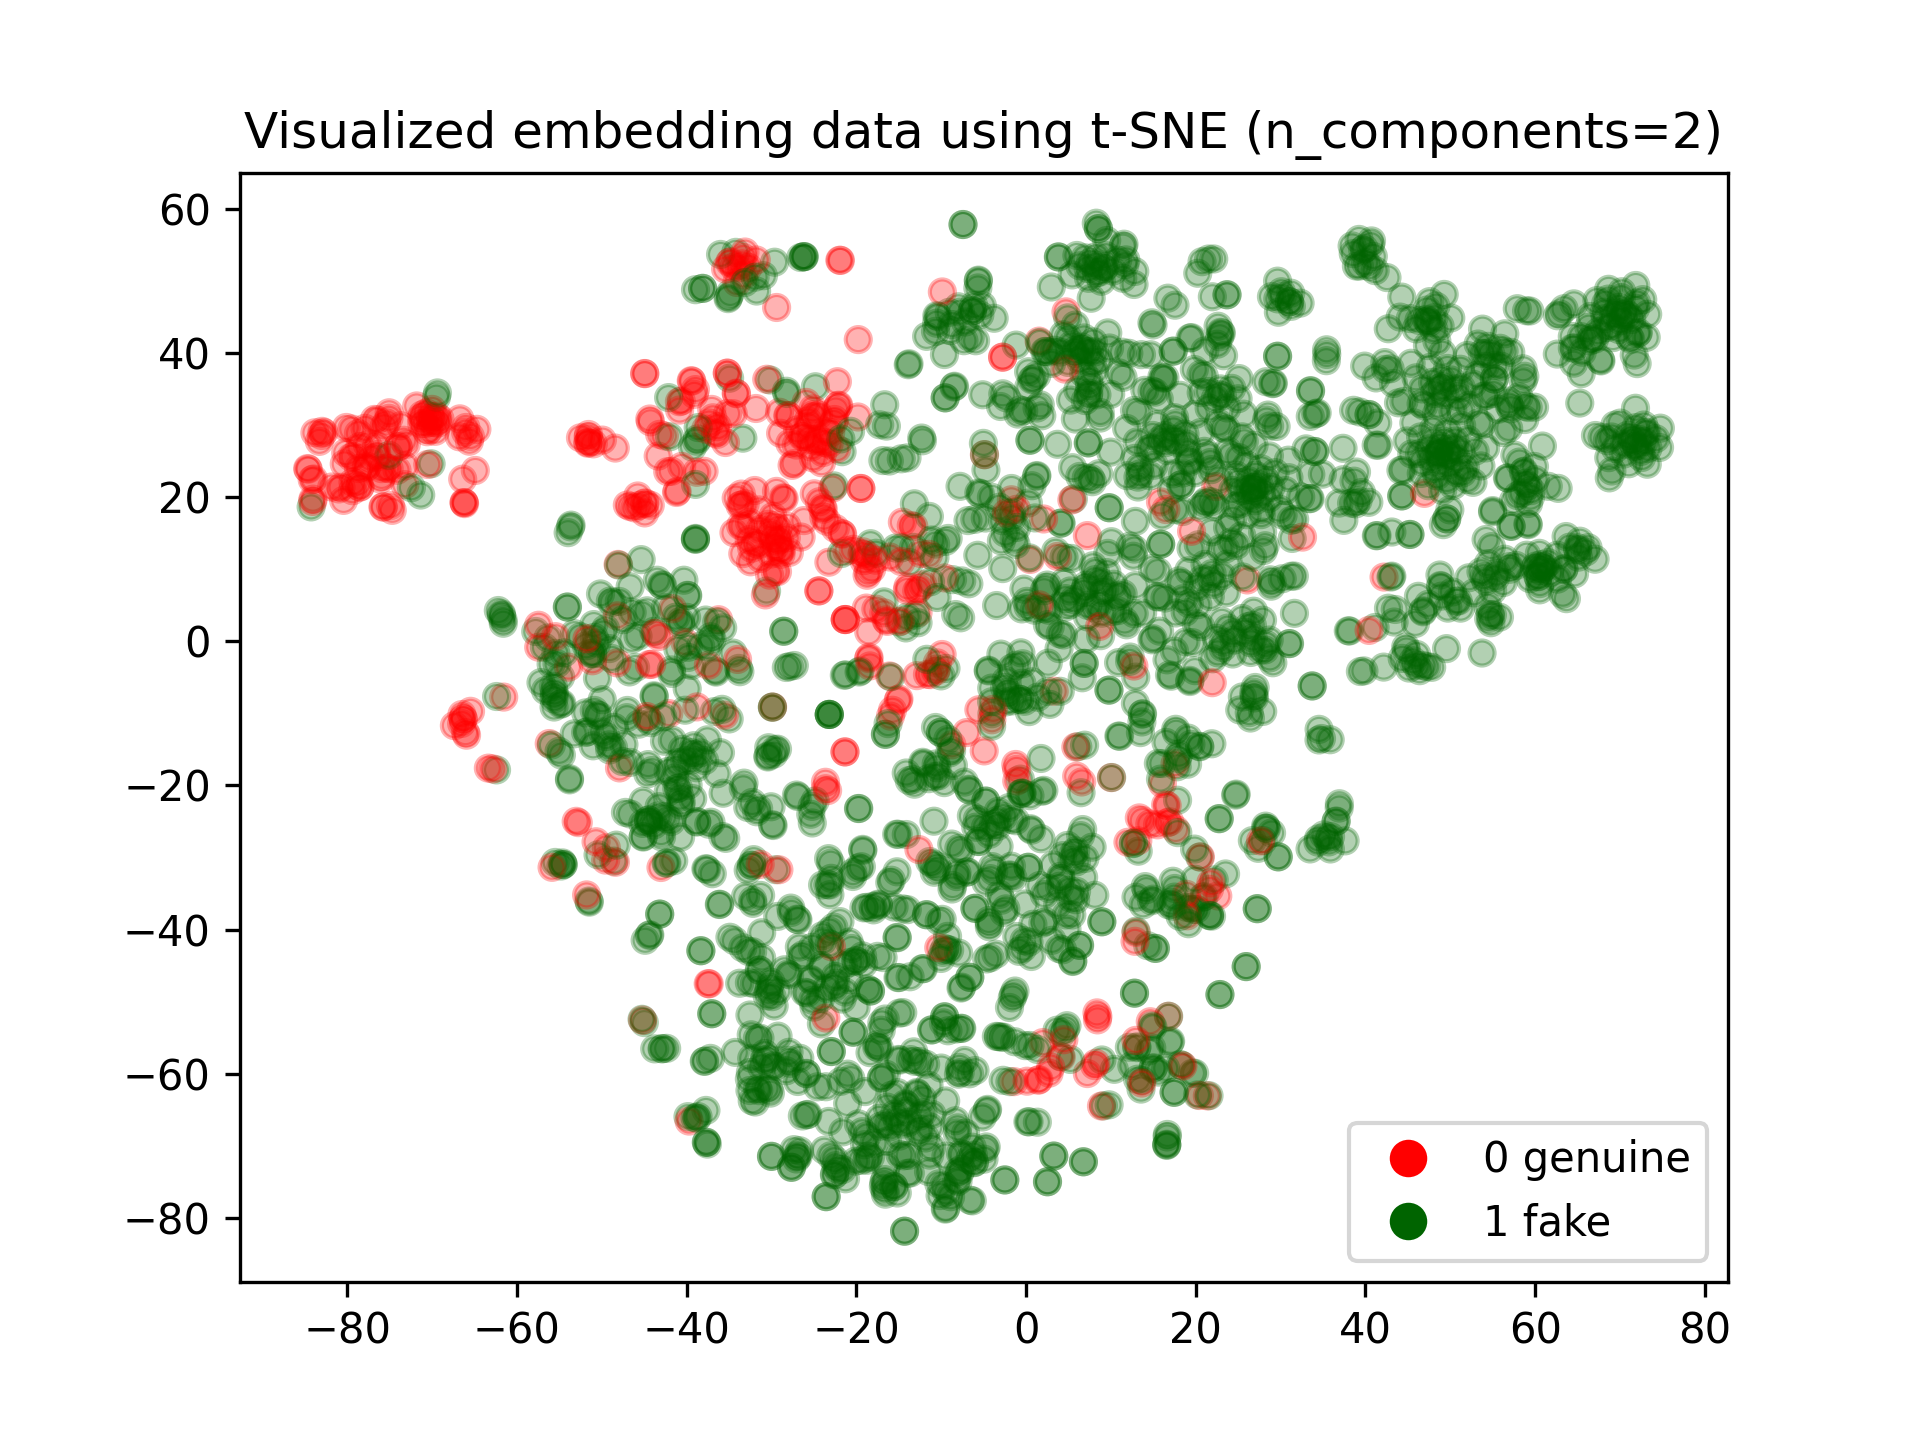
\includegraphics[width=1\linewidth]{img/ada_embedding.png}
    \caption{Visualization of text-embedding-ada-002 model using t-SNE}
    \label{fig:ada_embedding}
\end{figure}

These embeddings were then used as features with the machine learning method, such as SVM, for training. Incorporating knowledge from large language models with the training dataset enhances the accuracy of text classification predictions.
Additionally, OpenAI's GPT-4\cite{b29}, considered the state-of-the-art LLM, was directly employed to infer the texts in the test set. This procedure enables us to compare the performance of LLMs with the other methods in the study.

\section{Ensemble Methods}
Ensemble learning, a technique that combines the strengths of individual models, aims to generate predictions that surpass those of any single model. Traditional ensemble methods include soft voting and hard voting. Soft voting involves averaging the probabilities predicted by multiple classifiers and selecting the class with the highest average probability as the final prediction. On the other hand, hard voting selects the class with the majority of votes according to the hard labels from individual classifiers.\\

\subsection{Fuzzy rank-based ensemble method}
This study employed an approach to enhance prediction performance by combining the Gompertz function into ensemble learning techniques. Specifically, a fuzzy rank-based ensemble technique\cite{b30} was employed, which first considered each classifier's confidence in its predictions for each test case. This differs from conventional ensemble methods, such as average or weighted average rules, which assign pre-defined weights to classifiers. The re-parameterized Gompertz function(Fig. \ref{fig:Gompertz}) was included to compute the fuzzy ranks of each pre-trained model for detection. This method considers each model's predictions' uncertainty and confidence levels, leading to more precise results. To further enhance performance, PLMs like RoBERTa, DeBERTa, and XLNet were combined. These PLMs bring advanced language understanding capabilities to the ensemble, further improving the results.\\
\begin{figure}
    \centering
    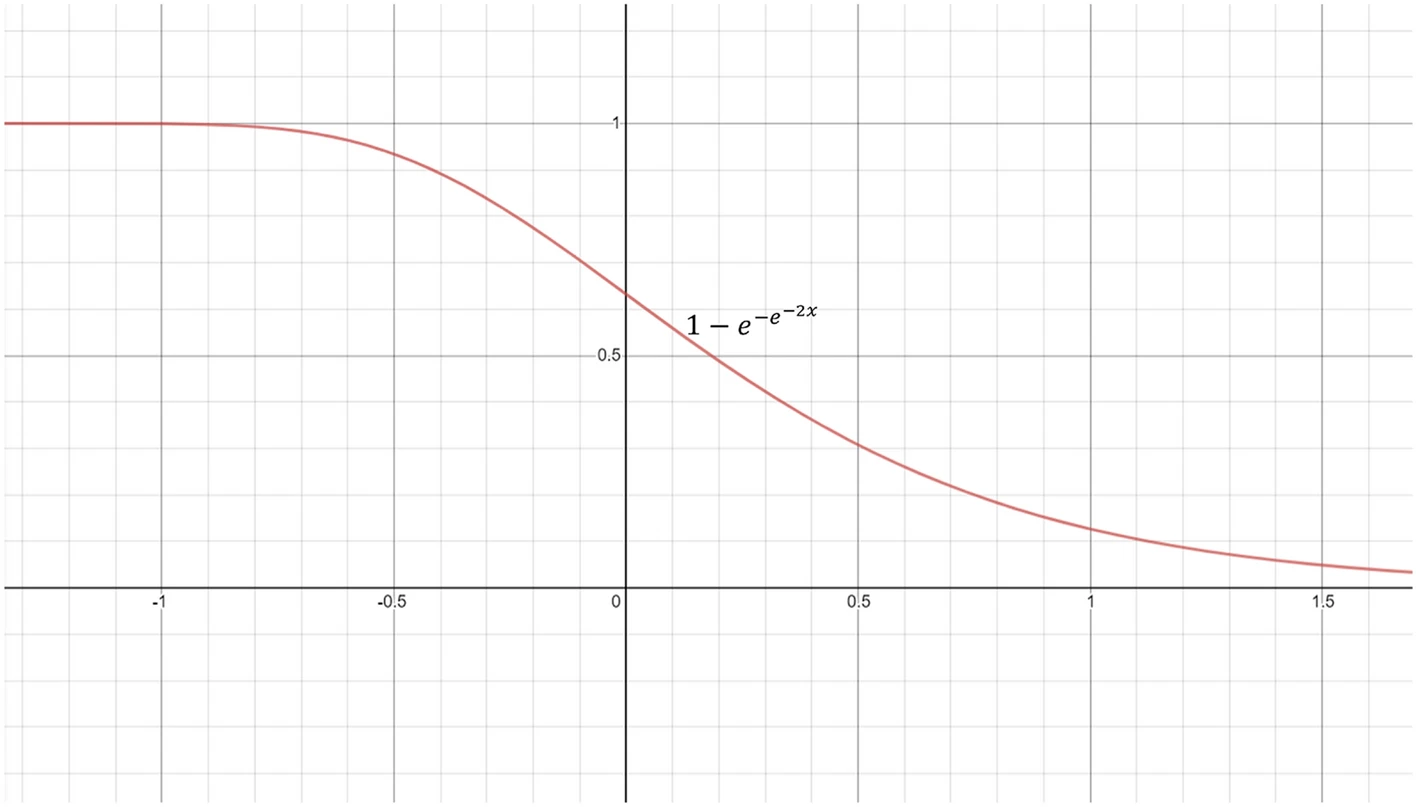
\includegraphics[width=1\linewidth]{img/Gompertz.png}
    \caption{The re-parameterized Gompertz function used in the fuzzy rank-based fusion method.\cite{b30}}
    \label{fig:Gompertz}
\end{figure}

Finally, the predictions of the three models (RoBERTa, DeBERTa, and XLNet) were fused using the fuzzy method, as illustrated in Fig. \ref{fig:process of proposed method}, providing the detailed process of the proposed method.

\begin{figure}
    \centering
    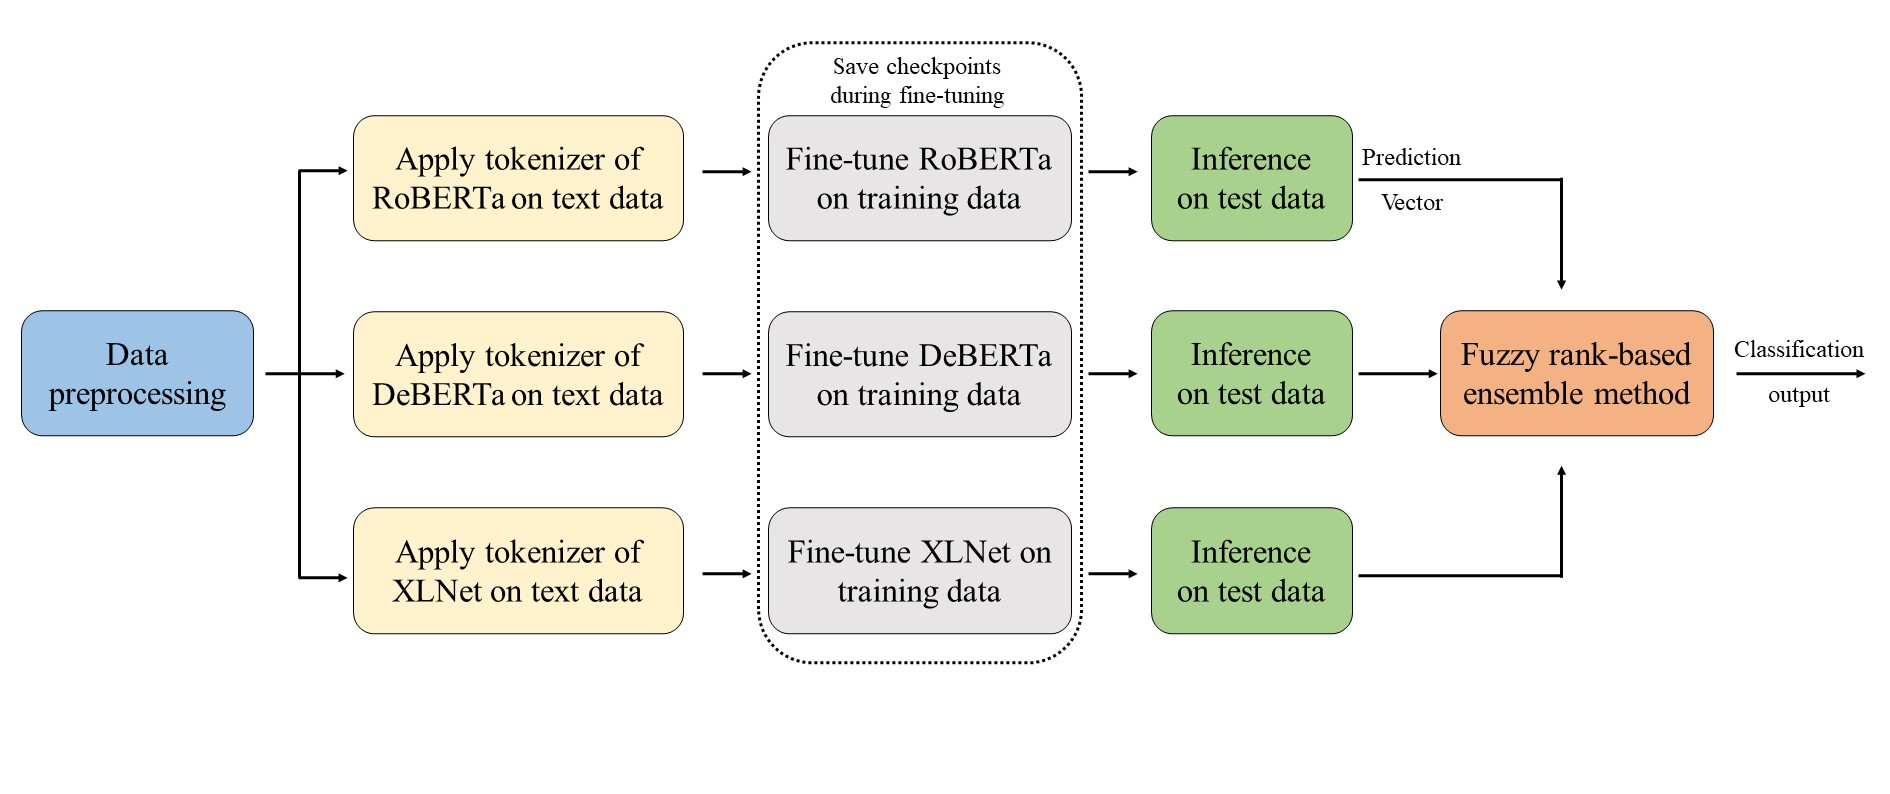
\includegraphics[width=1\linewidth]{img/process of proposed method.JPG}
    \caption{Flowchart of the fuzzy ensemble process using multiple language models.}
    \label{fig:process of proposed method}
\end{figure}

\subsection{Soft voting with content-based features}
The soft voting predicted probabilities were obtained from the RoBERTa, DeBERTa, and XLNet models. Each model assigned a probability to each class for a given instance, which was then averaged. Three content-based features described in Section 3.5.2 were incorporated into the soft voting ensemble method to compare the performance with the fuzzy method. These features were used to train an XGBoost model for final prediction (Fig. \ref{fig:process of content-based features method}). This strategy, which merged soft voting output with content-based features, was aimed at enhancing performance by providing additional context and detailed information, thereby improving classification accuracy. 

\begin{figure}
    \centering
    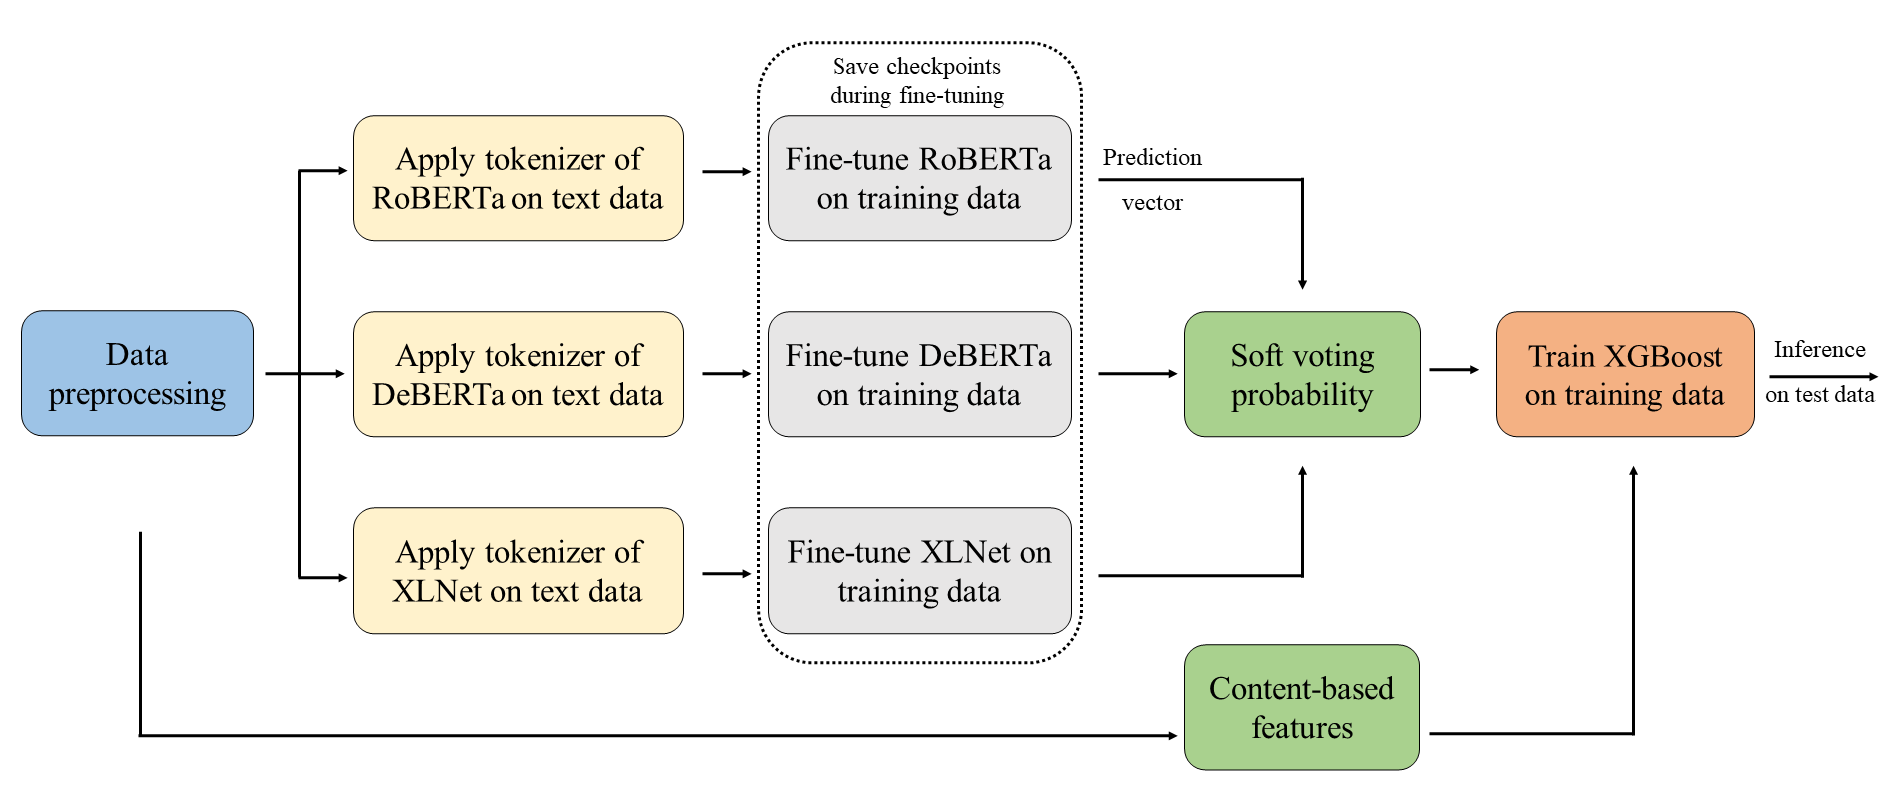
\includegraphics[width=1\linewidth]{img/soft voting with content-based features.png}
    \caption{Flowchart of training XGBoost with soft voting vector and content-based features.}
    \label{fig:process of content-based features method}
\end{figure}
 \newpage
\chapter{Experiments}
\label{ch:method}
\section{Implementation}
In the training phase, the stratified sampling approach was employed, where 10\% of the data was allocated for testing purposes and the remaining 90\% for training. The data was randomly split using the Scikit-learn package\cite{b31}. This strategy was selected to maintain consistent label proportions in the test and training sets. By doing so, we aimed to prevent the risk of insufficient genuine samples that could occur with random sampling.\\

The 5-fold cross-validation was implemented with Scikit-learn to train the SVM and XGBoost and determine the best-performing model for final evaluation. Fine-tuning of PLMs was conducted using checkpoints provided by Hugging Face, using the AdamW optimizer\cite{b32} and cross-entropy loss. The learning rate was set to 2e-5, and training was carried out for 20 epochs. HAN was trained for the same number of epochs with its default settings\cite{b33}. The training procedure was repeated five times with different random seeds, and checkpoints of models were selected for final evaluation based on the highest validation F1-score\cite{b34}. HAN was trained on the Tesla T4, while all other PLMs were trained on the RTX A5000.
\begin{figure}
  \centering
  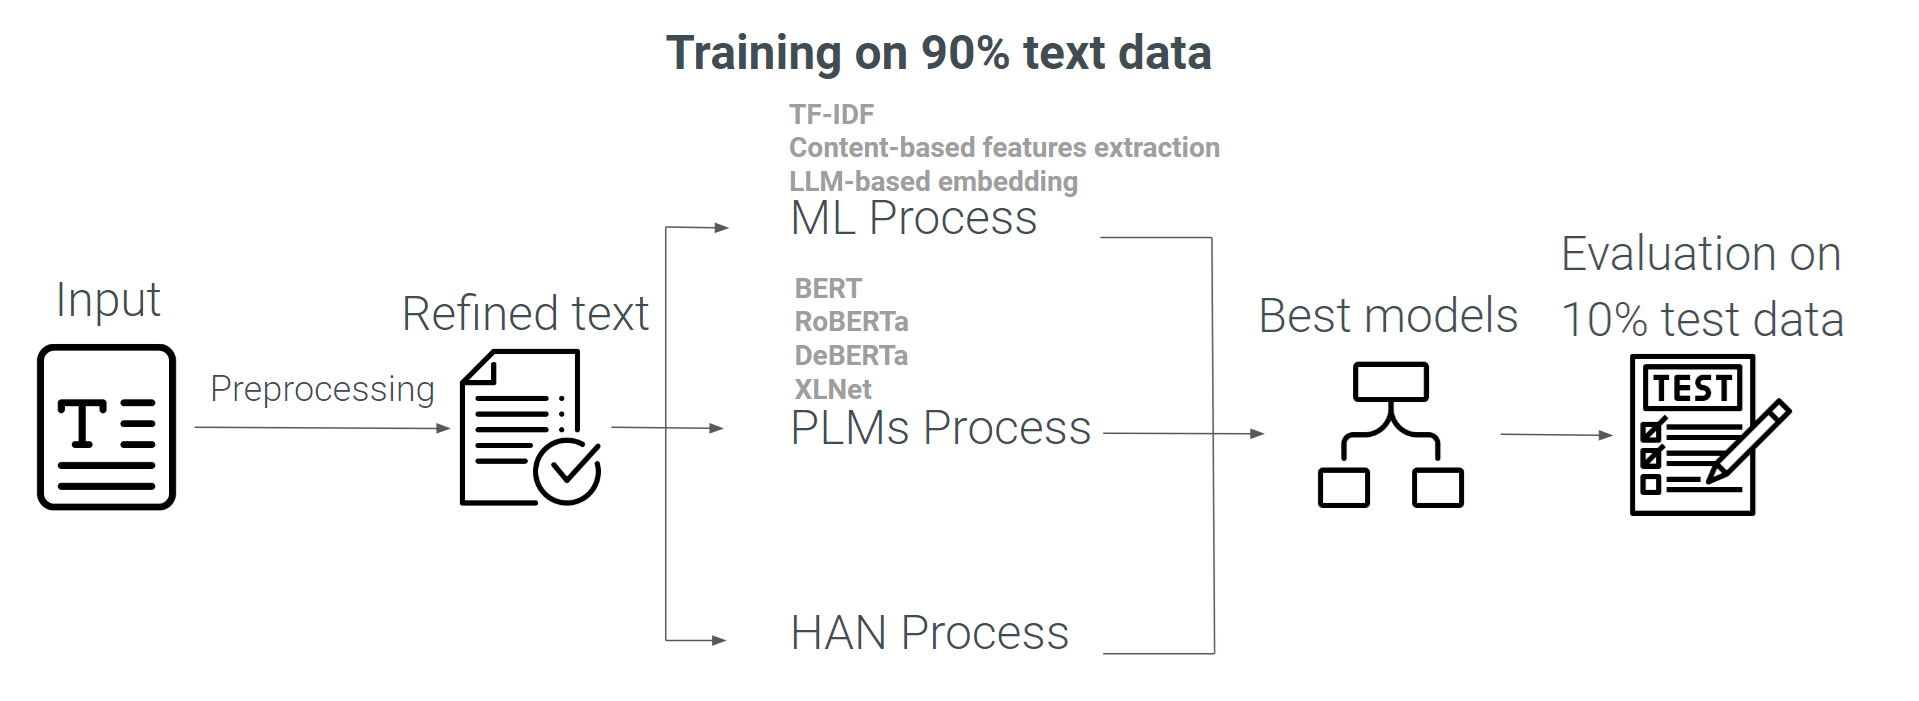
\includegraphics[width=1\columnwidth]{img/training2.png}
  \caption{The implementation workflow for the experiments. } 
  \vspace{-0.4cm}
  \label{fig:training}
\end{figure}
\\
The Fig. \ref{fig:training} illustrates the implementation workflow for the experiments. The model used the processed text as input and outputted a binary classification result (0 or 1), representing the categories of "genuine" or "fake". Finally, common metrics were calculated to evaluate the performance of the models.

\section{Configuration}
This study summarized the detailed information about implementation. For TF-IDF feature generations, the configurations illustrated in Table \ref{tab:TFIDF_detail} were used. Regarding implementations of the BERT series, the parameter settings were summarized as Table \ref{tab:BERT_detail} present. Acknowledging that changing parameter settings can result in diverse outcomes, we followed the configuration of the previous studies\cite{b5,b31,b33} to fine-tune the pre-trained models used in the experiments. This approach ensures that our models are optimized for performance and reliability across different scenarios and datasets.

\begin{table}
    \centering
    \caption{Parameter settings of TF-IDF features extractor.}
    \label{tab:TFIDF_detail}
\begin{tabular}{|c|c|}
\hline
Parameter     & Configuration \\ \hline
Stop\_words   & None          \\
Ngram\_range  & (1, 1)        \\
Min\_df       & 1             \\
Max\_features & None          \\ \hline
\end{tabular}
\end{table}


\begin{table}
    \centering
    \caption{Parameter settings for fine-tuning pretrained language models (PLMs)}
    \label{tab:BERT_detail}
\begin{tabular}{|c|cccc|}
\hline
Parameter      & BERT     & RoBERTa  & DeBERTa  & XLNet    \\ \hline
Max\_length    & 256      & 256      & 256      & 256      \\
Batch\_size    & 64       & 64       & 32       & 64       \\
Learning\_rate & 2e-5     & 2e-5     & 2e-5     & 2e-5     \\
Epochs         & 20       & 20       & 20       & 20       \\
Val\_metric    & F1-score & F1-score & F1-score & F1-score \\ \hline
\end{tabular}
\end{table}

\section{Evaluation metrics}
The concept of a confusion matrix is commonly used in classification tasks to evaluate the performance of machine learning models. It provides a detailed breakdown of the predictions made by the model compared to the actual ground truth. The confusion matrix consists of four primary elements:
\begin{itemize}
    \item True Positive (TP): These are the cases where the model correctly predicts the positive class.
    \item False Positive (FP): These are the cases where the model incorrectly predicts the positive class (i.e., predicts positive when the actual class is negative).
    \item True Negative (TN): These are the cases where the model correctly predicts the negative class.
    \item False Negative (FN): These are the cases where the model incorrectly predicts the negative class (i.e., predicts negative when the actual class is positive).
\end{itemize}

In evaluating the performance of classification models, several vital metrics such as accuracy, precision, recall, F1-score, and Area Under the Curve (AUC) are commonly used to provide a comprehensive assessment based on the confusion matrix. 

Accuracy is one of the famous metrics for classification tasks. This metric evaluates how often the model makes correct predictions by comparing the number of correctly predicted observations to the total number of observations. Accuracy can be calculated via the following formula:
\begin{equation}
    Accuracy = \frac{TP+TN}{TP+TN+FP+FN}
\end{equation}

% \subsection{Precision and Recall}
Precision is the ratio of correctly predicted positive observations to the total predicted positive observations, also known as the positive predictive value. Recall, or sensitivity, measures the ratio of correctly predicted positive observations to all actual positives. Precision and recall are calculated using:
\begin{equation}
    Precision = \frac{TP}{TP+FP}
\end{equation}
\begin{equation}
    Recall = \frac{TP}{TP+FN}
\end{equation}

% \subsection{F1-score}
F1-score balances precision and recall by taking their harmonic mean. It is beneficial when we need to consider both false positives and false negatives for a more accurate evaluation of model performance. This metric is particularly helpful when dealing with imbalanced datasets, providing a more accurate evaluation of the model's performance. The formula for F1-score is:
\begin{equation}
    F1\text{-}score = 2×\frac{Precision×Recall}{Precision+Recall}
\end{equation}

% \subsection{AUC}
The Area Under the Curve (AUC) measures the model's capability to distinguish between classes and is used as the summary of a receiver operating characteristic (ROC) curve. The ROC curve displays the model's determining ability as the discrimination threshold changes. A higher AUC value indicates a better ability of the model to distinguish between positive and negative instances correctly.

\section{Experimental results}
Model performances were evaluated using well-known metrics: accuracy, precision, recall, F1-score, and AUC. The results presented in Table \ref{tab:results} compare the proposed method with other approaches, including traditional machine learning algorithms, attention-based deep learning networks like HAN, pre-trained networks, and state-of-the-art LLMs. In addition, both the fuzzy rank-based method and soft voting method combine the RoBERTa, DeBERTa, and XLNet models.
\begin{table}[]
    \caption{ Comparison of the performance of different models for test data using various evaluation metrics includes accuracy, precision, recall, F1-score, and AUC.}
    \label{tab:results}
    \centering
\begin{tabular}{lccccc}
\hline
Model                   & Accuracy & Precision & Recall  & F1-score & AUC     \\ \hline
TF-IDF + SVM            & 89.08\%  & 91.46\%   & 95.34\% & 93.36\%  & 92.02\% \\
Engineered features + XGBoost        & 82.59\%  & 83.88\%   & 97.03\% & 89.98\%  & 78.95\% \\
HAN                     & 90.78\%  & 94.09\%   & 94.49\% & 94.29\%  & 93.09\% \\
BERT                    & 91.13\%  & 93.75\%   & 95.34\% & 94.54\%  & 96.31\% \\
RoBERTa                 & 91.81\%  & 93.44\%   & 96.61\% & 95.00\%  & 96.59\% \\
DeBERTa                 & 91.81\%  & 94.17\%   & 95.76\% & 94.96\%  & 95.75\% \\
XLNet                   & 92.83\%  & 94.24\%   & 97.03\% & 95.62\%  & 96.12\% \\
Ada-002 + SVM     & 92.83\%  & 93.52\%   & \textbf{97.88\%} & 95.65\%  & 94.88\% \\
Gemini + SVM  & 91.47\%  & 92.71\%   & 97.03\% & 94.82\%  & 93.27\% \\
GPT-4                   & 82.25\%  & 91.82\%   & 85.59\% & 88.60\%  & N/A     \\
Soft voting             & 93.17\%  & 94.63\%   & 97.03\% & 95.82\%  & 97.14\% \\
Soft voting with features       & 92.49\%  & 93.15\%   & \textbf{97.88\%} & 95.45\%  & 96.52\% \\
Fuzzy rank-based method & \textbf{93.52\%}  & \textbf{94.65\%}   & 97.46\% & \textbf{96.03\%}  & \textbf{97.15\%}     \\ \hline
\end{tabular}
\end{table}
\subsection{TF-IDF with SVM}
TF-IDF with SVM achieved an accuracy of 89.08\%, precision of 91.46\%, recall of 95.34\%, F1-score of 93.36\%, and AUC of 92.02\%. However, it is crucial to acknowledge that the performance of TF-IDF with SVM can be constrained when dealing with complex text data that need a deeper understanding of contextual data relationships. While these metrics show acceptable performance, they are still beaten by attention-based deep models like the HAN and BERT series in the experiments.

\subsection{Engineered features with XGBoost}
The use of sectarian words, the strength of quoted sources/attribution, and linguistic features provided a certain degree of accuracy in classifying long COVID-related fake news. However, due to differences in the dataset, our study lacked the inconsistency score feature used in the original methodology. Therefore, the performance of this approach in the experiments was lower than other methods. Specifically, except for recall, all other metrics were below the baseline. The experiment results indicate that while these content-based features contribute to the classification task, the absence of the inconsistency score limited the overall usefulness.
Additionally, this aligns with our prior data analysis, particularly the sentiment analysis. In section 3.4.2, the sentiment analysis showed that genuine and fake articles overlap in neutral sentiment and subjectivity categories, suggesting that these textual features alone are insufficient for accurate classification. The similar sentiment distribution across genuine and fake texts may contribute to the limitations observed in the content-based feature approach.

\subsection{HAN}
The HAN model achieved an accuracy of 90.78\%, precision of 94.09\%, recall of 94.49\%, F1-score of 94.29\%, and an AUC of 93.09\% in the experiment. This demonstrated that HAN performed well in the text classification task, maintaining reasonable recall and F1-score while achieving high accuracy and precision. Comparing HAN with TF-IDF and BERT, we can observe that HAN outperforms TF-IDF in terms of accuracy (90.78\% vs. 89.08\%), F1-score(94.29\% vs. 93.36\%), and AUC (93.09\% vs. 92.02\%), indicating its superior performance in the study. However, BERT achieved slightly higher accuracy (91.13\%) and AUC (96.31\%) compared to HAN.
\subsection{BERT series}
With its self-attention mechanism, BERT achieved a notable performance better than TF-IDF in the study, showing the advantages of BERT's self-attention mechanism in capturing complex patterns in the text data. It achieved an accuracy of 91.13\%, precision of 93.75\%, recall of 95.34\%, F1-score of 94.54\%, and AUC of 96.31\%. Another interesting observation in the experiments is that extensions of BERT, such as RoBERTa, DeBERTa, and XLNet, consistently outperformed the original BERT model. This phenomenon indicates the usefulness of their individual improvement strategies. Among the BERT series, XLNet stands out as the top performer.
\subsection{LLMs}
Gemini and text-embedding-ada-002, based on the advancements of LLMs, converted textual data into high-dimension embedding vectors and achieved F1-score of 94.82\% and 95.65\%, respectively. The text-embedding-ada-002 had a precision of 93.52\%, recall of 97.88\%, accuracy of 92.83\%, and AUC of 94.88\%, exhibiting its ability to distinguish between genuine and fake news effectively. Conversely, GPT-4, which was directly used for text classification, had an accuracy of 82.25\%, indicating that its performance could have been more competitive than other models in the experiment. However, the performance was still acceptable even without training and fine-tuning. Due to the use of the GPT-4 API, it was not possible to properly obtain the model's probabilities for predicting fake and genuine labels, making the calculation of the AUC infeasible.
\subsection{Ensemble methods}
Last but not least, the ensemble methods, including soft voting and the fuzzy rank-based method, demonstrated their effectiveness by achieving F1-score of 95.82\% and 96.03\% in the experiments, respectively. These results outperformed individual models like conventional TF-IDF and state-of-the-art LLM, emphasizing the power of combining information from multiple models for enhanced final decision-making in text classification tasks. Especially the fuzzy method achieved impressive results on the test set, with an accuracy of 93.52\%, precision of 94.65\%, F1-score of 96.03\%, and AUC of 97.15\%, presenting the highest performance among all methods estimated. Fig. \ref{fig:confusion matrix} shows the confusion matrix with the top 4 F1-score in the experiment.
\begin{figure}
    \centering
    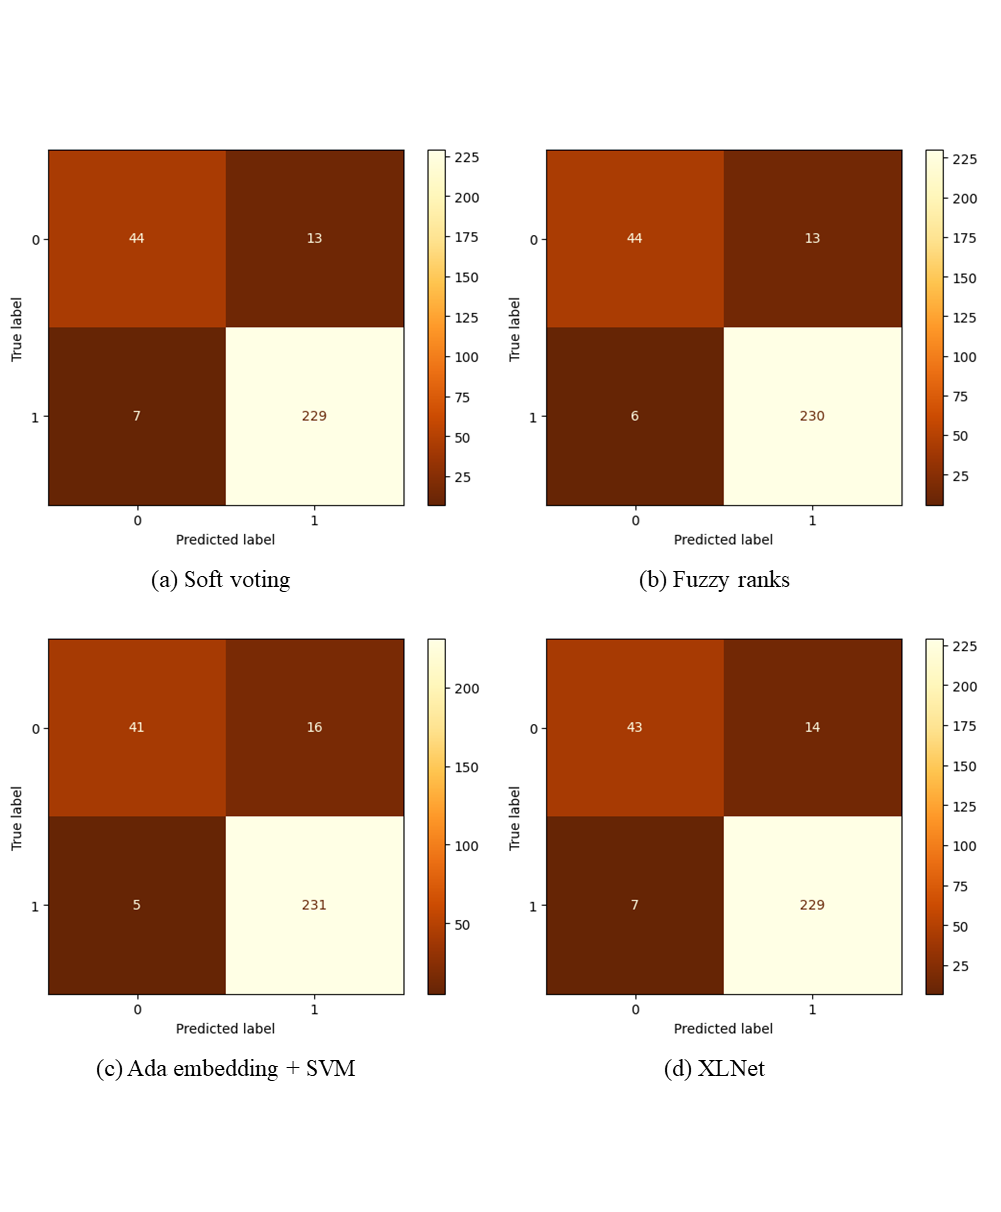
\includegraphics[width=1\linewidth]{img/CM4.png}
    \caption{Confusion matrix of (a) soft voting, (b) fuzzy rank-based method, (c) Ada embedding method and (d)XLNet on the held-out test dataset.}
    \label{fig:confusion matrix}
\end{figure}

On the other hand, despite attempting to enhance the classification ability by incorporating sectarian words, the strength of quoted sources/attribution, and linguistic features with soft voting probabilities, the experimental results indicated otherwise. Except for a slight improvement in recall, other metrics showed a minor decline. In contrast, the fuzzy rank-based ensemble method, which combines predictions from multiple models, demonstrated superior performance.
The possible explanation for this outcome is that different attention-based models already include information similar to the content-based features. Therefore, the absence of the inconsistency score introduced noise, adversely affecting the model's performance. This suggests that while content-based features are valuable, their effectiveness is diminished when the attention-based models already capture similar information.





\section{Real case inference}

Table \ref{tab:real case} is the actual case of using the fuzzy method to detect fake and genuine news that was not included in the test set. We used four isolated samples, two genuine and two fake, varying in short and long length. The result shows that our method accurately detected the genuineness of the content regardless of its length, revealing its robustness across different text lengths.


\begin{table}[]
    \caption{Real case inference using fuzzy rank ensemble method.}
    \label{tab:real case}
    \centering
\begin{tabular}{|l|c|c|c|}
\hline
\rowcolor[HTML]{31394D} 
{\color[HTML]{FFFFFF} Content / Mainly claim}                                                                                                                                                                                                                                                                                                                                                                                                                                                                                                                                                                                                                                                        & \multicolumn{1}{l|}{\cellcolor[HTML]{31394D}{\color[HTML]{FFFFFF} Length}} & \multicolumn{1}{l|}{\cellcolor[HTML]{31394D}{\color[HTML]{FFFFFF} Prediction}} & \multicolumn{1}{l|}{\cellcolor[HTML]{31394D}{\color[HTML]{FFFFFF} Ground truth}} \\ \hline
\begin{tabular}[c]{@{}l@{}}A German study has revealed long COVID is linked\\  to the vaccine.\end{tabular}                                                                                                                                                                                                                                                                                                                                                                                                                                                                                                                                                                                          & 15                                                                         & fake                                                                           & fake                                                                             \\ \hline
\begin{tabular}[c]{@{}l@{}}Covid vaccination before infection strongly linked to\\  reduced risk of developing long covid\end{tabular}                                                                                                                                                                                                                                                                                                                                                                                                                                                                                                                                                               & 15                                                                         & genuine                                                                        & genuine                                                                          \\ \hline
\begin{tabular}[c]{@{}l@{}}Long COVID's causes and risk factors remain a subject\\  of ongoing research, with potential factors including\\  reactivation of SARS-CoV-2 particles, overactive \\ immune responses, and the development of \\ autoantibodies attacking organs. Certain groups, such as\\  those with severe COVID-19 history, underlying health\\  conditions, or lacking vaccination, are at higher risk, \\ alongside other factors like sex, age, initial immune\\  response, and viral variants. Health inequities may\\  also contribute, especially affecting racial or ethnic \\ minority groups and individuals with disabilities.\end{tabular}                               & 367                                                                        & genuine                                                                        & genuine                                                                          \\ \hline
\begin{tabular}[c]{@{}l@{}}While Omicron's subvariants find new ways to \\ evade vaccines and destabilize immune systems, \\ another pandemic has overwhelmed offcials who \\ are supposed to be in charge of public health. \\ In any case, COVID, a novel virus that can wreak \\ havoc with vital organs in the body, continues \\ to evolve at a furious pace. In response officials have \\ largely abandoned any coherent response, including \\ masking, testing, tracing and even basic data collection.\\  Yes, the people have been abandoned. So don't expect \\ "normal" to return to your hospital, your airport, your \\ nation, your community or your life anytime soon.\end{tabular} & 469                                                                        & fake                                                                           & fake                                                                             \\ \hline
\end{tabular}
\end{table} \newpage
\chapter{Discussion and Conclusion}
\label{ch:evaluation}
\section{Discussion}
\subsection{Principal findings}
The experiment results provide some insights into the impact of model parameters on classification performance. As observed in Table \ref{tab:parameters}, models with more parameters generally achieve better classification accuracy. For instance, BERT, RoBERTa, DeBERTa, and XLNet, which have significantly more parameters than HAN, demonstrate superior performance across various evaluation metrics such as accuracy, precision, recall, F1-score, and AUC. \\

\begin{table}[]
    \caption{Parameters of each deep model used in the study.}
    \label{tab:parameters}
    \centering
\begin{tabular}{lc}
\hline
Model                                         & \multicolumn{1}{l}{Parameters} \\ \hline
HAN                                           & 2,343,202                      \\
BERT                                          & 109,483,778                    \\
RoBERTa                                       & 124,647,170                    \\
DeBERTa                                       & 139,193,858                    \\
XLNet                                         & 117,310,466                    \\
{\color[HTML]{666666} text-embedding-ada-002}    & {\color[HTML]{666666} unknown} \\
{\color[HTML]{666666} Gemini-embedding} & {\color[HTML]{666666} unknown} \\
{\color[HTML]{666666} GPT-4}                  & {\color[HTML]{666666} unknown} \\ \hline
\end{tabular}
\end{table}

Despite having a lower parameter count than other PLMs, XLNet still achieved better performance among the BERT series in the experiment. This outcome implies that not just the number of parameters but also the model architecture, training process, and optimization techniques are essential in determining classification effectiveness. XLNet's success could be attributed to its permutation language modeling approach, which allows for enhanced bidirectional context understanding while addressing some of the limitations of bidirectional models like BERT.\\

\subsection{LLM-based embedding models}
Additionally, using LLM-based embedding models exhibits superior performance compared to traditional TF-IDF features. However, accessing embedding models through OpenAI's API needs charges, while the Gemini API only offers limited-time free trials. Although the exact number of parameters for the text-embedding-ada-002 model, Gemini embedding model, and GPT-4 is not formally disclosed, it can be assumed that these models likely have a larger parameter count compared to the other open-source PLMs like BERT, RoBERTa, DeBERTa, and XLNet. In this study, text-embedding-ada-002 performed slightly better than Gemini, possibly due to differences in the length of the embedding vectors. GPT defaults to 1536 dimensions, while Gemini is set at 768. Despite yielding acceptable outcomes, directly using GPT-4 falls short compared to training SVM on vector-transformed training data using embedding models. This suggests that LLMs still benefit from training data in classification tasks. \\

\subsection{Overall}
The LLM-based embedding models showed remarkable performance in the experiment. However, the fuzzy method can be combined with open-source PLMs to achieve even better results. Moreover, compared to using a single language model or soft voting method with pre-defined weights, the fuzzy fusion-based technique allows for determining ensemble model weights for each test case, resulting in superior performance.\\

The experiment results underscore the importance of model architecture and size in determining classification effectiveness. While smaller models like HAN can still perform well, larger and more parameter-rich models like BERT variants and XLNet demonstrate the potential for even higher accuracy and robustness, given their capability to learn complicated patterns and representations from the textual data via attention mechanism. However, it is worth noting that the computational and resource requirements also increase significantly with larger models. A balance between model complexity and practical feasibility is required in real-world applications.

\subsection{Limitations}
One limitation of the study is the presence of data imbalance. Although identical samples were removed, the dataset might have included samples of similar misinformation forwarded using different wording. The imbalance in the data also implies a potential bias towards the prevalence of fake information on the internet. Addressing this issue would require gathering a more extensive and up-to-date dataset of genuine information to achieve better balance and representativeness in the training data. \\

Another limitation is the dependence on a single label to categorize content related to long COVID-19. Different health policies in certain countries may restrain this approach, leading to potential misclassification or oversimplification of complicated information. There may need to be more than a single label for classification to accurately differentiate the nuances of such content. The future incorporation of generative AI models like GPT-4 and Llama\cite{b35} could be a game-changer. With appropriate training and fine-tuning, LLMs can learn real-world information, thus offering accurate and detailed content identification. These models have the potential to distinguish between truthful and false segments within an article, improving the usefulness of detecting misinformation related to long COVID and reinfection. This advancement could significantly improve media literacy among the public.

\subsection{Future work}
Future efforts can involve fine-tuning open-source LLMs like Meta's Llama and the Alpaca model from the Stanford University team\cite{b36} to improve misinformation detection further. These Generative AI (GAI) models have various advantages, particularly their ability to explore deeper than binary classifications of genuine or fake content. Through comprehensive training or fine-tuning, these language models can tell which sections contain accurate or false information within an article.
Moreover, developing image-text models\cite{b37} becomes important since some social media content involves multimodal information, such as videos and images. Image-text models could combine image and textual inputs, offering a complete approach to misinformation detection. This method can provide more support in real-world situations.\\

Furthermore, data augmentation techniques could provide helpful help during training. Traditional augmentation methods in NLP, such as translations\cite{b38} and innovative augmentations via LLMs\cite{b39}, offer more balanced and diverse training data. These augmentation strategies could enhance the model's robustness and generalization capabilities, improving performance in detecting misinformation.

\section{Conclusion}
This study used open-source databases and reputable websites to collect textual data concerning long-term COVID and reinfections. Through information engineering techniques, we gained insights into the characteristics of articles and claims about these topics. AI models, including attention-based models and linear classifiers, have shown strength in detecting misleading or inaccurate information, serving as valuable tools for the public to discern between genuine and fake information. Unlike traditional models that treat all parts of the input equally, attention-based models can focus on relevant information while ignoring irrelevant or noisy data. This allows the model to prioritize important features and contextually relevant elements, leading to more accurate predictions. \\

Besides, ensemble methods have demonstrated robust performance by minimizing prediction errors' variance and reducing dispersion. The fuzzy rank-based fusion method with PLMs and the Gompertz function presents a helpful approach to prediction methodologies, offering potential improvements in accuracy and reliability. Moreover, experimental results indicate that training solely on textual content can achieve high prediction performance.
 \newpage
% \chapter{Discussion and Conclusion}
% \label{ch:conclusion}

% \section{Discussion}
% \subsection{Principal findings}
% The experiment results provide some insights into the impact of model parameters on classification performance. As observed in Table \ref{tab:parameters}, models with more parameters generally achieve better classification accuracy. For instance, BERT, RoBERTa, DeBERTa, and XLNet, which have significantly more parameters than HAN, demonstrate superior performance across various evaluation metrics such as accuracy, precision, recall, F1-score, and AUC. \\

% \begin{table}[]
%     \caption{Parameters of each deep model used in the study.}
%     \label{tab:parameters}
%     \centering
% \begin{tabular}{lc}
% \hline
% Model                                         & \multicolumn{1}{l}{Parameters} \\ \hline
% HAN                                           & 2,343,202                      \\
% BERT                                          & 109,483,778                    \\
% RoBERTa                                       & 124,647,170                    \\
% DeBERTa                                       & 139,193,858                    \\
% XLNet                                         & 117,310,466                    \\
% {\color[HTML]{666666} text-embedding-ada-002}    & {\color[HTML]{666666} unknown} \\
% {\color[HTML]{666666} Gemini-embedding} & {\color[HTML]{666666} unknown} \\
% {\color[HTML]{666666} GPT-4}                  & {\color[HTML]{666666} unknown} \\ \hline
% \end{tabular}
% \end{table}

% Despite having a lower parameter count than other PLMs, XLNet still achieved better performance among the BERT series in the experiment. This outcome implies that not just the number of parameters but also the model architecture, training process, and optimization techniques are essential in determining classification effectiveness. XLNet's success could be attributed to its permutation language modeling approach, which allows for enhanced bidirectional context understanding while addressing some of the limitations of bidirectional models like BERT.\\

% \subsection{LLM-based embedding models}
% Additionally, using LLM-based embedding models exhibits superior performance compared to traditional TF-IDF features. However, accessing embedding models through OpenAI's API needs charges, while the Gemini API only offers limited-time free trials. Although the exact number of parameters for the text-embedding-ada-002 model, Gemini embedding model, and GPT-4 is not formally disclosed, it can be assumed that these models likely have a larger parameter count compared to the other open-source PLMs like BERT, RoBERTa, DeBERTa, and XLNet. In this study, text-embedding-ada-002 performed slightly better than Gemini, possibly due to differences in the length of the embedding vectors. GPT defaults to 1536 dimensions, while Gemini is set at 768. Despite yielding acceptable outcomes, directly using GPT-4 falls short compared to training SVM on vector-transformed training data using embedding models. This suggests that LLMs still benefit from training data in classification tasks. \\

% \subsection{Overall}
% The LLM-based embedding models showed remarkable performance in the experiment. However, the fuzzy method can be combined with open-source PLMs to achieve even better results. Moreover, compared to using a single language model or soft voting method with pre-defined weights, the fuzzy fusion-based technique allows for determining ensemble model weights for each test case, resulting in superior performance.\\

% The experiment results underscore the importance of model architecture and size in determining classification effectiveness. While smaller models like HAN can still perform well, larger and more parameter-rich models like BERT variants and XLNet demonstrate the potential for even higher accuracy and robustness, given their capability to learn complicated patterns and representations from the textual data via attention mechanism. However, it is worth noting that the computational and resource requirements also increase significantly with larger models. A balance between model complexity and practical feasibility is required in real-world applications.

% \subsection{Limitations}
% One limitation of the study is the presence of data imbalance. The imbalance in the data suggests a potential bias towards the prevalence of fake information on the internet. Addressing this issue would require gathering a more extensive and up-to-date dataset of genuine information to achieve better balance and representativeness in the training data. \\

% Another limitation is the dependence on a single label to categorize content related to long COVID-19. Different health policies in certain countries may restrain this approach, leading to potential misclassification or oversimplification of complicated information. There may need to be more than a single label for classification to accurately differentiate the nuances of such content. The future incorporation of generative AI models like GPT-4 and Llama\cite{b35} could be a game-changer. With appropriate training and fine-tuning, LLMs can learn real-world information, thus offering accurate and detailed content identification. These models have the potential to distinguish between truthful and false segments within an article, improving the usefulness of detecting misinformation related to long COVID and reinfection. This advancement could significantly improve media literacy among the public.

% \subsection{Future work}
% Future efforts can involve fine-tuning open-source LLMs like Meta's Llama and the Alpaca model from the Stanford University team\cite{b36} to improve misinformation detection further. These Generative AI (GAI) models have various advantages, particularly their ability to explore deeper than binary classifications of genuine or fake content. Through comprehensive training or fine-tuning, these language models can tell which sections contain accurate or false information within an article.
% Moreover, developing image-text models\cite{b37} becomes important since some social media content involves multimodal information, such as videos and images. Image-text models could combine image and textual inputs, offering a complete approach to misinformation detection. This method can provide more support in real-world situations.\\

% Furthermore, data augmentation techniques could provide helpful help during training. Traditional augmentation methods in NLP, such as translations\cite{b38} and innovative augmentations via LLMs\cite{b39}, offer more balanced and diverse training data. These augmentation strategies could enhance the model's robustness and generalization capabilities, improving performance in detecting misinformation.

% \section{Conclusion}
% This study used open-source databases and reputable websites to collect textual data concerning long-term COVID and reinfections. Through information engineering techniques, we gained insights into the characteristics of articles and claims about these topics. AI models, including attention-based models and linear classifiers, have shown strength in detecting misleading or inaccurate information, serving as valuable tools for the public to discern between genuine and fake information. Unlike traditional models that treat all parts of the input equally, attention-based models can focus on relevant information while ignoring irrelevant or noisy data. This allows the model to prioritize important features and contextually relevant elements, leading to more accurate predictions. \\

% Besides, ensemble methods have demonstrated robust performance by minimizing prediction errors' variance and reducing dispersion. The fuzzy rank-based fusion method with PLMs and the Gompertz function presents a helpful approach to prediction methodologies, offering potential improvements in accuracy and reliability. Moreover, experimental results indicate that training solely on textual content can achieve high prediction performance. \newpage
% =========================================================================


% =========================================================================
% 參考文獻的檔案 Reference file: ref.bib
%\ClearShipoutPicture % 把ref的浮水印關掉

\iftoggle{toc-use-cn} % 使用中文
{\addcontentsline{toc}{chapter}{參考文獻}
\renewcommand{\bibname}{參考文獻} } 
{\addcontentsline{toc}{chapter}{References}
\renewcommand{\bibname}{References}
} 

\bibliographystyle{IEEEtran}
\begin{thebibliography}{00}
\bibitem{b1}“Infodemic.” Accessed: Sep. 28, 2023. [Online]. Available: https://www.who.int/health-topics/infodemic
\bibitem{b2}H. E. Davis, L. McCorkell, J. M. Vogel, and E. J. Topol, “Long COVID: major findings, mechanisms and recommendations,” Nat. Rev. Microbiol., vol. 21, no. 3, Art. no. 3, Mar. 2023, doi: 10.1038/s41579-022-00846-2.
\bibitem{b3}B. Bowe, Y. Xie, and Z. Al-Aly, “Acute and postacute sequelae associated with SARS-CoV-2 reinfection,” Nat. Med., vol. 28, no. 11, Art. no. 11, Nov. 2022, doi: 10.1038/s41591-022-02051-3.
\bibitem{b4}P. Patwa et al., “Fighting an Infodemic: COVID-19 Fake News Dataset,” vol. 1402, 2021, pp. 21–29. doi: 10.1007/978-3-030-73696-5\_3.
\bibitem{b5}S. D. Das, A. Basak, and S. Dutta, “A Heuristic-driven Ensemble Framework for COVID-19 Fake News Detection.” arXiv, Jan. 10, 2021. doi: 10.48550/arXiv.2101.03545.
\bibitem{b6}W. S. Paka, R. Bansal, A. Kaushik, S. Sengupta, and T. Chakraborty, “Cross-SEAN: A cross-stitch semi-supervised neural attention model for COVID-19 fake news detection,” Appl. Soft Comput., vol. 107, p. 107393, Aug. 2021, doi: 10.1016/j.asoc.2021.107393.
\bibitem{b7}C. Yang, X. Zhou, and R. Zafarani, “CHECKED: Chinese COVID-19 fake news dataset,” Soc. Netw. Anal. Min., vol. 11, no. 1, p. 58, Jun. 2021, doi: 10.1007/s13278-021-00766-8.
\bibitem{b8}“ChatGPT.” Accessed: Oct. 19, 2023. [Online]. Available: https://chat.openai.com
\bibitem{b9}“covid\_fake\_news/data at main · diptamath/covid\_fake\_news,” GitHub. Accessed: Oct. 18, 2023. [Online]. Available: https://github.com/diptamath/covid\_fake\_news/tree/main/data
\bibitem{b10}L. Cui and D. Lee, “CoAID: COVID-19 Healthcare Misinformation Dataset.” arXiv, Nov. 03, 2020. doi: 10.48550/arXiv.2006.00885.
\bibitem{b11}J. Kim, J. Aum, S. Lee, Y. Jang, E. Park, and D. Choi, “FibVID: Comprehensive fake news diffusion dataset during the COVID-19 period,” Telemat. Inform., vol. 64, p. 101688, Nov. 2021, doi: 10.1016/j.tele.2021.101688.
\bibitem{b12}S. Sharma, E. Agrawal, R. Sharma, and A. Datta, “FaCov: COVID-19 Viral News and Rumors Fact-Check Articles Dataset,” Proc. Int. AAAI Conf. Web Soc. Media, vol. 16, pp. 1312–1321, May 2022, doi: 10.1609/icwsm.v16i1.19383.
\bibitem{b13}“COVID Archives | Snopes.com.” Accessed: Oct. 19, 2023. [Online]. Available: https://www.snopes.com/tag/covid-19/
\bibitem{b14}“Fact-checks | PolitiFact.” Accessed: Oct. 19, 2023. [Online]. Available: https://www.politifact.com/factchecks/list/?category=coronavirus
\bibitem{b15}J. Y. Khan, Md. T. I. Khondaker, S. Afroz, G. Uddin, and A. Iqbal, “A benchmark study of machine learning models for online fake news detection,” Mach. Learn. Appl., vol. 4, p. 100032, Jun. 2021, doi: 10.1016/j.mlwa.2021.100032.

\bibitem{b16}“TextBlob: Simplified Text Processing — TextBlob 0.16.0 documentation.” Accessed: Oct. 12, 2023. [Online]. Available: https://textblob.readthedocs.io/en/dev/

\bibitem{b17}C. Cortes and V. Vapnik, “Support-vector networks,” Mach. Learn., vol. 20, no. 3, pp. 273–297, Sep. 1995, doi: 10.1007/BF00994018.

\bibitem{b18}Y.-C. Lin, S.-A. Chen, J.-J. Liu, and C.-J. Lin, “Linear Classifier: An Often-Forgotten Baseline for Text Classification,” in Proceedings of the 61st Annual Meeting of the Association for Computational Linguistics (Volume 2: Short Papers), Toronto, Canada: Association for Computational Linguistics, Jul. 2023, pp. 1876–1888. doi: 10.18653/v1/2023.acl-short.160.

\bibitem{b19} Abu Salem FK, Al Feel R, Elbassuoni S, Ghannam H, Jaber M, Farah M. Meta-learning for fake news detection surrounding the Syrian war. Patterns. 2021;2(11):100369. doi:10.1016/j.patter.2021.100369

\bibitem{b20}Z. Yang, D. Yang, C. Dyer, X. He, A. Smola, and E. Hovy, “Hierarchical Attention Networks for Document Classification,” in Proceedings of the 2016 Conference of the North American Chapter of the Association for Computational Linguistics: Human Language Technologies, San Diego, California: Association for Computational Linguistics, 2016, pp. 1480–1489. doi: 10.18653/v1/N16-1174.

\bibitem{b21}J. Devlin, M.-W. Chang, K. Lee, and K. Toutanova, “BERT: Pre-training of Deep Bidirectional Transformers for Language Understanding.” arXiv, May 24, 2019. doi: 10.48550/arXiv.1810.04805.

\bibitem{b22}Vaswani A, Shazeer N, Parmar N, et al. Attention Is All You Need. Published online August 1, 2023. doi:10.48550/arXiv.1706.03762

\bibitem{b23}Y. Liu et al., “RoBERTa: A Robustly Optimized BERT Pretraining Approach.” arXiv, Jul. 26, 2019. doi: 10.48550/arXiv.1907.11692.

\bibitem{b24}P. He, X. Liu, J. Gao, and W. Chen, “DeBERTa: Decoding-enhanced BERT with Disentangled Attention.” arXiv, Oct. 06, 2021. doi: 10.48550/arXiv.2006.03654.

\bibitem{b25}Z. Yang, Z. Dai, Y. Yang, J. Carbonell, R. R. Salakhutdinov, and Q. V. Le, “XLNet: Generalized Autoregressive Pretraining for Language Understanding,” in Advances in Neural Information Processing Systems, Curran Associates, Inc., 2019. Accessed: Jul. 12, 2023. [Online]. Available: https://papers.nips.cc/paper\_files/paper/2019/hash/dc6a7e655d7e5840e\\66733e9ee67cc69-Abstract.html

\bibitem{b26}New and improved embedding model. Accessed March 25, 2024. https://openai.com/blog/new-and-improved-embedding-model

\bibitem{b27}Gemini Team, Anil R, Borgeaud S, et al. Gemini: A Family of Highly Capable Multimodal Models. Published online December 18, 2023. doi:10.48550/arXiv.2312.11805

\bibitem{b28}Maaten L van der, Hinton G. Visualizing Data using t-SNE. J Mach Learn Res. 2008;9(86):2579-2605.

\bibitem{b29}OpenAI, “GPT-4 Technical Report.” arXiv, Mar. 27, 2023. Accessed: Dec. 04, 2023. [Online]. Available: http://arxiv.org/abs/2303.08774

\bibitem{b30}Kundu R, Basak H, Singh PK, Ahmadian A, Ferrara M, Sarkar R. Fuzzy rank-based fusion of CNN models using Gompertz function for screening COVID-19 CT-scans. Sci Rep. 2021;11(1):14133. doi:10.1038/s41598-021-93658-y

\bibitem{b31}F. Pedregosa et al., “Scikit-learn: Machine Learning in Python,” J. Mach. Learn. Res., vol. 12, no. 85, pp. 2825–2830, 2011.

\bibitem{b32}Loshchilov I, Hutter F. Decoupled Weight Decay Regularization. Published online January 4, 2019. doi:10.48550/arXiv.1711.05101

\bibitem{b33}richliao/textClassifier: Text classifier for Hierarchical Attention Networks for Document Classification. Accessed May 4, 2024. https://github.com/richliao/textClassifier/tree/master

\bibitem{b34}I. Chalkidis et al., “LexGLUE: A Benchmark Dataset for Legal Language Understanding in English,” in Proceedings of the 60th Annual Meeting of the Association for Computational Linguistics (Volume 1: Long Papers), Dublin, Ireland: Association for Computational Linguistics, May 2022, pp. 4310–4330. doi: 10.18653/v1/2022.acl-long.297.

\bibitem{b35}Touvron H, Lavril T, Izacard G, et al. LLaMA: Open and Efficient Foundation Language Models. Published online February 27, 2023. doi:10.48550/arXiv.2302.13971

\bibitem{b36}Stanford CRFM. Accessed May 1, 2024. https://crfm.stanford.edu/2023/03/13/alpaca.html

\bibitem{b37}Chen Z, Du Y, Hu J, et al. Mapping medical image-text to a joint space via masked modeling. Med Image Anal. 2024;91:103018. doi:10.1016/j.media.2023.103018

\bibitem{b38}Shorten C, Khoshgoftaar TM, Furht B. Text Data Augmentation for Deep Learning. J Big Data. 2021;8(1):101. doi:10.1186/s40537-021-00492-0

\bibitem{b39}Chintagunta B, Katariya N, Amatriain X, Kannan A. Medically Aware GPT-3 as a Data Generator for Medical Dialogue Summarization. In: Proceedings of the Second Workshop on Natural Language Processing for Medical Conversations. Association for Computational Linguistics; 2021:66-76. doi:10.18653/v1/2021.nlpmc-1.9
\end{thebibliography}
%========================================================================

% \chapter*{Supplemental information}
% \addcontentsline{toc}{chapter}{Supplemental information}
% \section*{A. Model architecture}
% \begin{figure}[H]
%     \centering
%     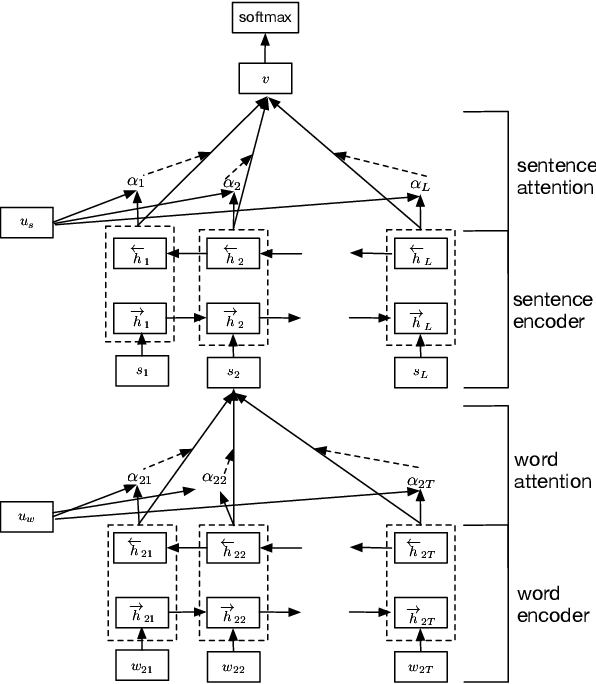
\includegraphics[width=0.85\linewidth]{img/HAN.png}
%     \caption{Architecture of Hierarchical Attention Networks(HAN)\cite{b19}}
%     \label{fig:HAN architecture}
% \end{figure}

%=========================================
% \section*{B. Implementation details}
% We summarized the detailed information about implementation. For TF-IDF feature generations, we used the configurations illustrated in Table \ref{tab:TFIDF_detail}. Regarding implementations of the BERT series, we summarize the parameter settings as Table \ref{tab:BERT_detail} present. We acknowledge that changing parameter settings can result in diverse outcomes. Therefore, we followed the configuration of the previous studies\cite{b5,b31,b33} to fine-tune the pre-trained models used in the experiments. This approach ensures that our models are optimized for performance and reliability across different scenarios and datasets.

% \begin{table}[H]
%     \centering
%     \caption{Parameter settings of TF-IDF features extractor.}
%     \label{tab:TFIDF_detail}
% \begin{tabular}{|c|c|}
% \hline
% Parameter     & Configuration \\ \hline
% Stop\_words   & None          \\
% Ngram\_range  & (1, 1)        \\
% Min\_df       & 1             \\
% Max\_features & None          \\ \hline
% \end{tabular}
% \end{table}


% \begin{table}[H]
%     \centering
%     \caption{Parameter settings of PLMs.}
%     \label{tab:BERT_detail}
% \begin{tabular}{|c|cccc|}
% \hline
% Parameter      & BERT     & RoBERTa  & DeBERTa  & XLNet    \\ \hline
% Max\_length    & 256      & 256      & 256      & 256      \\
% Batch\_size    & 64       & 64       & 32       & 64       \\
% Learning\_rate & 2e-5     & 2e-5     & 2e-5     & 2e-5     \\
% Epochs         & 20       & 20       & 20       & 20       \\
% Val\_metric    & F1-score & F1-score & F1-score & F1-score \\ \hline
% \end{tabular}
% \end{table}
% \newpage
%=========================================
% \section*{C. Confusion matrix}
% This section shows the remaining confusion matrices, excluding the top four methods mentioned in Chapter 5.
% \begin{figure}[H]
%     \centering
%     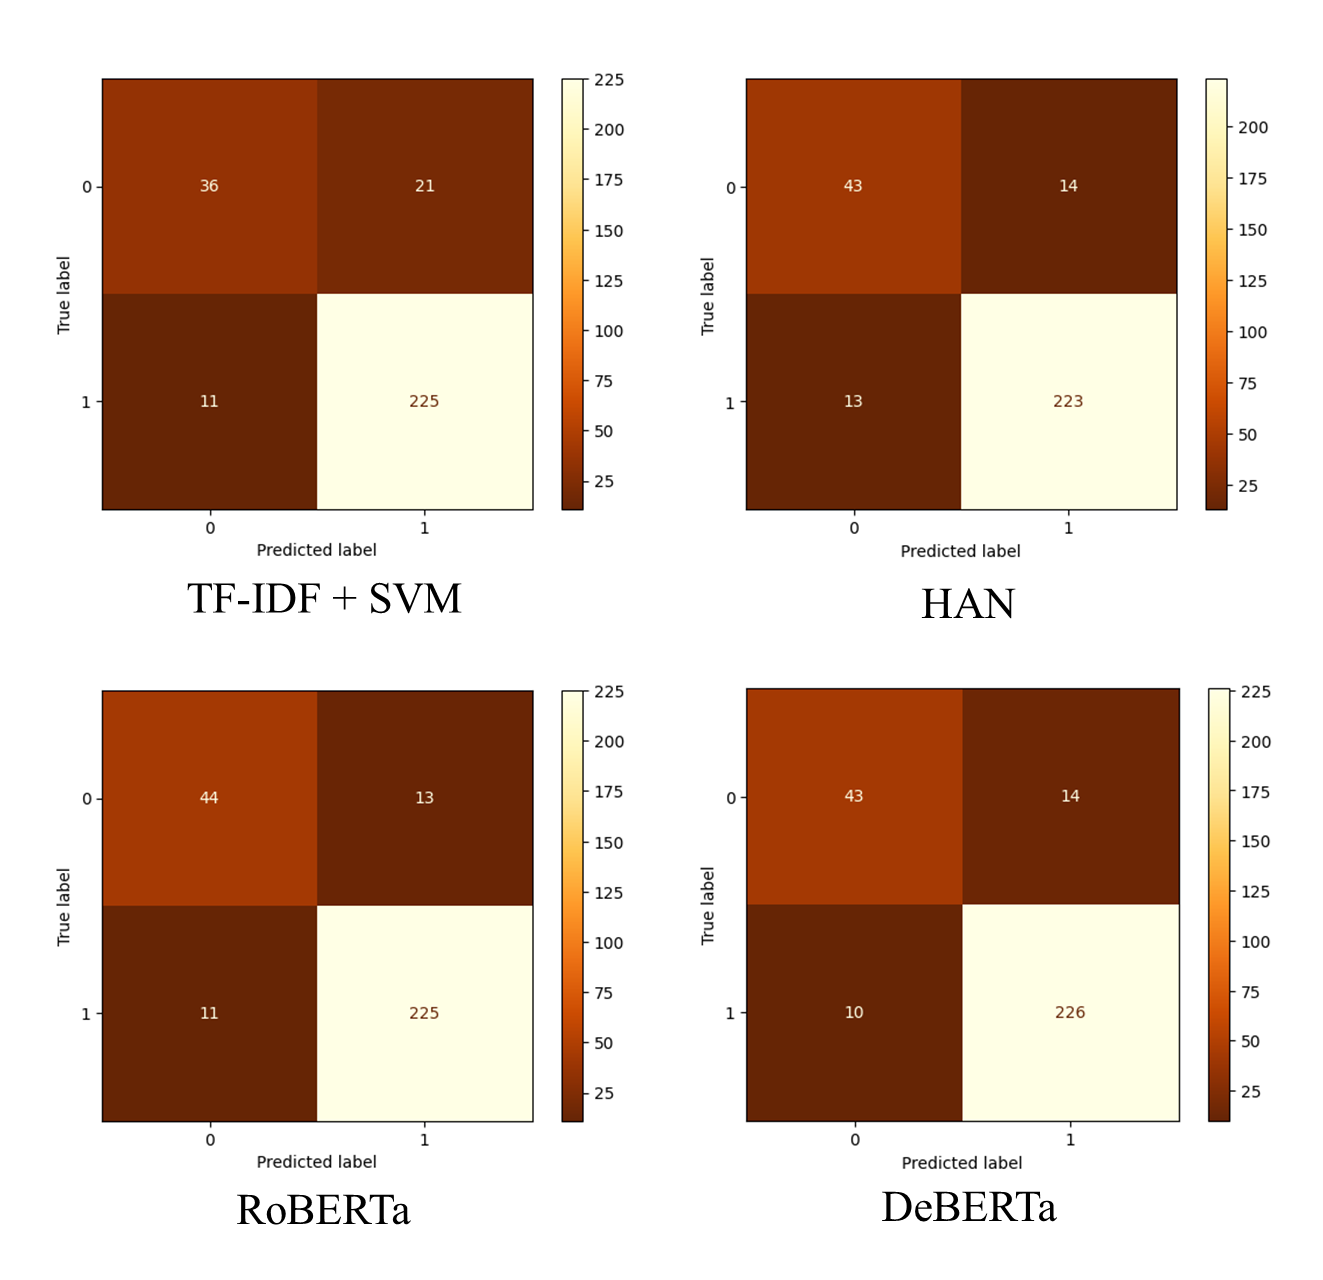
\includegraphics[width=1\linewidth]{img/TF+HAN+Ro+De.png}
%     \caption{Confusion matrix of TF-IDF, HAN, RoBERTa and DeBERTa on test dataset.}
%     \label{fig:Supplementary_CM1}
% \end{figure}

% \begin{figure}[H]
%     \centering
%     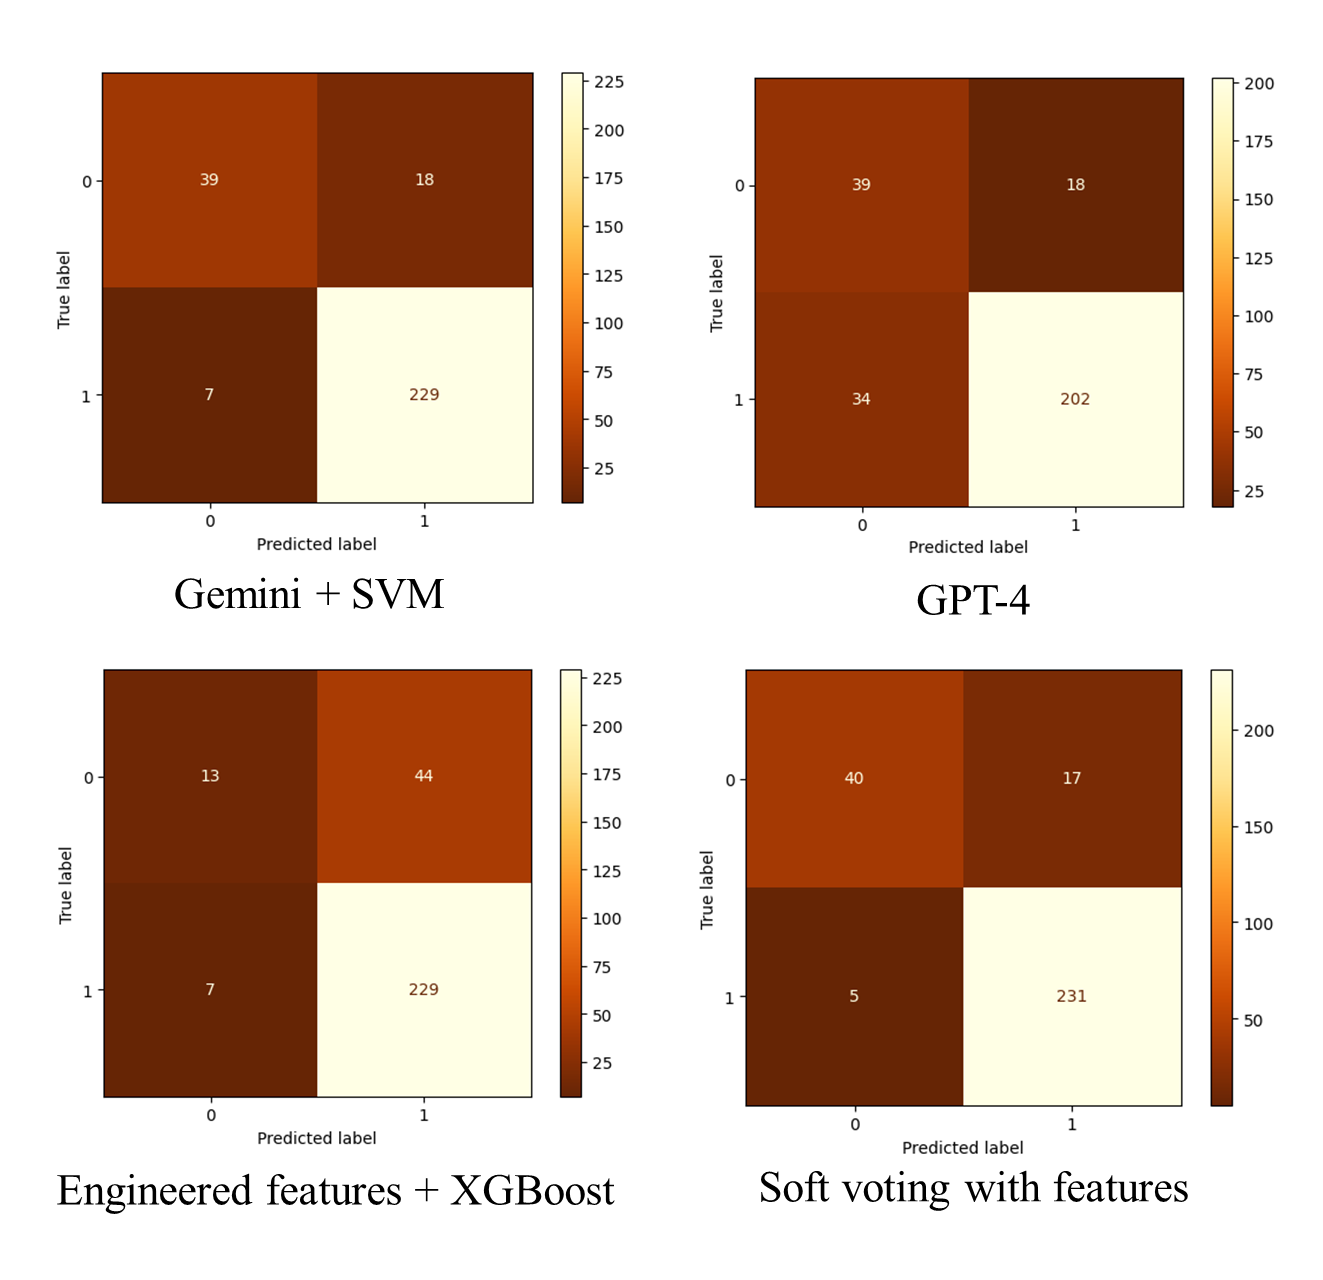
\includegraphics[width=1\linewidth]{img/Gemini+GPT4+EF.png}
%     \caption{Confusion matrix of Gemini+SVM, GPT-4 and engineered features methods on test dataset.}
%     \label{fig:Supplementary_CM2}
% \end{figure}

% =========================================================================

% NYCU參考資料:
% 臺灣博碩士論文知識加值系統 https://ndltd.ncl.edu.tw/
% 學位論文編寫事項 https://www.lib.nycu.edu.tw/custom_label?menu=64&lid=6
% 各學院、系所學位中英文名稱 https://aa.nycu.edu.tw/reg/統計資訊/
% 圖書館FB: https://www.facebook.com/NYCULIB



\end{CJK*}
\balance

\end{document}
